\documentclass[a4,12pt]{book}

\usepackage{template}

% Parallelepiped definitions

%should be compiled with xelatex to use special fonts

\begin{document}


%%%%%%%%%%%%%%%%%%%%%%%%%%%%%%%%%%%%%%%%%%%%%%%%
%redefining chapter appearence for introduction
\titleformat{\chapter} % redefining chapter appearence
%{} % style
{\titlefont\Huge\bf} % style
{} % label
{0pt} % separation
{\begin{tikzpicture}[remember picture,overlay]
    \filldraw [x=1mm,y=1mm, special, overlay] (37,0) circle [radius=9];
    \filldraw [x=1mm,y=1mm, attention, overlay] (58,0) circle [radius=9];
    \filldraw [x=1mm,y=1mm, light, overlay] (79,0) circle [radius=9];
    \filldraw [x=1mm,y=1mm, common, overlay] (210,-9) -- (100 ,-9) arc (-90:-270:9) --(100,9)
    -- (210,9); %(118, 0) node{\color{white} Lição \thechapter} (105,-27);
  \end{tikzpicture}
} % before title
[\vspace{3cm} \hfill{\bf\bigtitlefont\raggedright\color{special} #1}] % after title
%\titlespacing*{\chapter}{0pt}{50pt}{100pt} % {<command>}{<left>}{<before-sep>}{<after-sep>}
%%%%%%%%%%%%%%%%%%%%%%%%%%%%%%%%%%%%%%%%%%%%%%%%%%%%%%%%%%%%%%%%%%%%%%%%%%%%%%%%%%%%%%%%%%%%%

%%%%%%%%%%%%%%%%%%%%%%%%%%%%%%%%%%%%%%%%%%%%%%%%%%%%%%%%%%%%%%%%%%%%%%%%%%%%%%%%%%%%%%%%%%%%
% Footers for introduction
\fancyfoot[C]{%
\noindent%
\tikz[baseline]{\draw[color=ref, line width=0.6pt] (-0.5, 0) -- (6, 0);}%
}

% Left footer
\fancyfoot[LE]{
  {\tikz{\draw[color=attention, line width=0.6pt] (-1.8, 0) -- (\textwidth, 0);}}\newline
  {\tikz[x=1mm,y=1mm]{\filldraw [attention, overlay] (-20,-3) -- (-5 ,-3)
      arc (-90:90:3) --(-5,3) -- (-20,3) (-8, 0) node{\color{white} {\bf \thepage}};}}
  {\small\color{dark} \leftmark}
}

% Right footer
\fancyfoot[RO]{
  {\tikz{\draw[color=attention, line width=0.6pt] (-1.8, 0) -- (\textwidth, 0);}}\newline
  {\small\color{dark} \leftmark}
  {\tikz[x=1mm,y=1mm]{\filldraw [attention, overlay] (20,-3) -- (5 ,-3)
      arc (-90:-270:3) --(5,3) -- (20,3) (8, 0) node{\color{white} {\bf \thepage}};}}
}%


\fancyfoot[C]{}
%%%%%%%%%%%%%%%%%%%%%%%%%%%%%%%%%%%%%%%%%%%%%%%%%%%%%%%%%%%%%%%%%%%%%%%%%%%%%%%%%%%%%
\frontmatter %to set pagenumbering roman in introduction

% \documentclass[a4,12pt,openany]{book}
%
% \usepackage{template_introducao}
%
% \begin{document}

\setcounter{chapter}{-1}
\chapter{Introdução}


<<<<<<< HEAD
Frações é certamente um dos tópicos que mais desafia o ensino e a aprendizagem de matemática da Educação Básica. Justamente por isso, tanto se publicou sobre o assunto nas últimas décadas (para citar apenas algumas das mais utilizadas:  {\it Rational Number Project, Institute of Education Science} (\cite{IES}, 2010), Van de Walle (\cite{Walle}, 2009) e Wu (\cite{Wu}, 2011). Este texto, organizado como uma proposta didática,  reúne as reflexões e as discussões dos autores sobre o tema, amparadas por essas publicações e pela análise de livros didáticos de diversos países. A proposta aqui apresentada foi planejada para:
=======
O assunto frações é certamente um dos tópicos que mais desafia o ensino e a aprendizagem na matemática da educação básica. Justamente por isso, tanto se publicou sobre o assunto nas últimas décadas (para citar apenas algumas das referências mais utilizadas:  {\it Rational Number Project, Institute of Education Science}, 2010 [7], Van de Walle, 2009 [29] e Wu, 2011 [31]). Este texto, organizado como uma proposta didática,  reúne as reflexões e as discussões dos autores sobre o tema, amparadas por essas publicações e pela análise de livros didáticos de diversos países. A proposta aqui apresentada foi planejada para:
>>>>>>> bcee628c638363fca63ed51180808d1c7305b477

\begin{enumerate}[(i)]
\item  ser aplicada diretamente em sala de aula, como material didático destinado aos anos intermediários do ensino fundamental (do $4^{\textrm{\underline{o}}}$ ao $7^{\textrm{\underline{o}}}$ ano) e
\item amparar a formação e o desenvolvimento profissional do professor que ensina matemática na educação básica.
\end{enumerate}

O texto concentra-se na abordagem inicial de frações como objeto matemático, buscando explorar o assunto a partir de atividades que visam à construção conceitual do tema e a conduzir os alunos a desenvolverem o raciocínio matemático amparados por reflexão e por discussão. Assim, as atividades visam a desafiar os alunos e a levá-los a estabelecer suas próprias conclusões sobre os assuntos tratados. Busca-se valorizar a capacidade cognitiva dos alunos, respeitando uma organização crescente e articulada de dificuldade na organização das atividades. Espera-se com isso mudar a perspectiva do binômio quantidade/qualidade. No lugar de uma quantidade enorme de exercícios, são propostas poucas  atividades que exigem maior reflexão e aprofundamento dos conceitos. Assim, são evitadas atividades de simples observação e repetição de modelos e os tradicionais ``exercícios de fixação'', que, pontuais, são apenas com o objetivo de desenvolver a fluência em procedimentos específicos (por exemplo, os que envolvem a equivalência entre frações).

Uma outra característica particular deste material é o diálogo com o professor. No início de cada lição, há uma introdução dirigida especificamente ao professor que apresenta os objetivos da lição, uma discussão dos aspectos matemáticos que serão tratados, as dificuldades esperadas e algumas observações sobre os passos cognitivos envolvidos. Diferente dos livros didáticos tradicionais, em que, para o professor, há pequenas observações pontuais junto ao texto do aluno e um longo texto teórico anexo ao final do livro, nesta proposta a ``conversa'' com o professor é permanente. Em cada atividade são realizadas discussões sobre os objetivos a serem alcançados, recomendações e sugestões metodológicas para sua execução e, quando pertinente, uma discussão sobre algum desdobramento do assunto tratado.

% Incluir aqui as descrições das seções de cada lição (Explorando o Assunto, Organizando as Ideias, Mão na Massa, Quebrando a Cuca e Refletindo).

Entende-se que, nesta etapa da escolaridade, considerando o cotidiano próprio do aluno, o conceito de fração aparece ligado a  noções informais traduzidas por expressões como metade, terço, quartos, décimos e centésimos, por exemplo. Assim, nas primeiras duas lições, buscou-se utilizar a linguagem verbal e os conhecimentos anteriores dos estudantes sobre situações em que aquelas expressões são utilizadas para conduzir as primeiras abordagens, visando à introdução de um conhecimento mais organizado e formal sobre o assunto. Apenas posteriormente, são introduzidas a linguagem e a simbologia próprias da matemática.

%Rever à luz do arquivo do GDocs
A introdução das frações na Educação Básica amplia o universo numérico do aluno e envolve um salto cognitivo, ir além da contagem. São duas as principais questões nesse processo: ``a identificação de uma unidade não explícita \textit{a priori}'' e a compreensão de uma  ``unidade contínua'', isto é, que pode ser subdividida em qualquer número de partes.

A construção de ideias abstratas, especialmente nesta etapa da escolaridade, deve ser amparada por contextos e modelos representativos. Na abordagem aqui proposta decidimos por iniciar apenas a partir de situações que envolvem modelos contínuos (linhas e regiões do plano ou do espaço). Assim, por exemplo, não trataremos de ``um terço de uma caixa de lápis'', mas de ``um terço de uma barra de chocolate''. 

A decisão por evitar modelos discretos em um momento inicial deve-se aos seguintes fatos: (i) modelos discretos já evidenciam uma unidade a priori; por exemplo, na determinação de um terço de 24 lápis, a unidade ``lápis'' não é nem a unidade nem a subunidade que precisam ser levadas em conta para a determinação da fração ``um terço de 24 lápis'' e (ii) como o conceito de fração subentende o de equipartição, contextos discretos podem desencadear discussões mais complexas, por exemplo, o que seria determinar $1/10$ de uma caixa de 24 lápis?

A opção por modelos contínuos traz limitações inerentes. É natural que os estudantes associem a fração à forma que a identifica no modelo. É necessário que identifique-se a fração não à forma, mas à quantidade evidenciada na representação. Assim, por exemplo, se o modelo for um retângulo, o que está em questão é a área e a fração $1/4$ pode ser representada igualmente por um retângulo ou um triângulo, como na figura a seguir (ver Atividade 4 da Lição 1).

Iniciar o estudo de frações a partir de modelos contínuos é uma decisão compartilhada por propostas que caracterizam livros japoneses e franceses.

\begin{center}
  \begin{tikzpicture}[scale=5]
  \draw[fill=common, fill opacity=.3] (15,0) rectangle (19,3);
  \draw[fill=common, fill opacity=.3] (15,3) rectangle (19,6);
  \draw (15,1.5) -- (19,1.5);
  \draw (15,3) -- (19,6);    
  \end{tikzpicture}
\end{center}

As lições 1 e 2 introduzem os conceitos elementares e a linguagem de frações a partir de situações concretas e de modelos contínuos. Na lição 1, as frações emergem de situações concretas amparadas pela linguagem verbal. Uma vez estabelecida a unidade, a expressão ``fração unitária'' nomeia cada uma das partes da divisão da unidade em partes iguais. Nas atividades dessas lições a unidade está fortemente vinculada a um objeto concreto. Assim, por exemplo, a fração de uma torta, não é ainda tratada com a abstração própria do conceito de número, mas como uma fatia da torta em uma equipartição. Toma-se bastante cuidado com o papel da determinação da unidade e com a necessidade de uma ``equipartição'' para a identificação de uma fração. A notação simbólica de frações e as frações não unitárias, incusive as maiores do que a unidade, surgem apenas na Lição 2. As frações com numerador diferente de 1 são apresentadas a partir da justaposição de frações unitárias com mesmo denominador ou simplesmente contando-se essas frações. Para isso, tem-se a representação pictórica como um apoio importante. Nessas lições, as atividades são quase majoritariamente para identificar, reconhecer, analisar e justificar.

Na Lição 3, é exigida maior abstração dos alunos. Retoma-se a representação de números na reta numérica, enfatizando, no contexto das frações, a associação do segmento unitário à unidade. Os modelos contínuos e a justaposição de partes correspondentes às frações unitárias são a base da proposta desenvolvida. A representação das frações na reta numérica é usada para amparar a abordagem da comparação de frações com um mesmo numerador e com um mesmo denominador. Além disso, são propostas atividades que tratam a comparação de frações a partir de uma referência.

A Lição 4 trata da equivalência de frações tendo como objetivo a sua função na comparação de duas frações quaisquer. O assunto é abordado utilizando-se representações equivalentes em modelos de área retangulares, em modelos de área circulares e na reta numérica. A inclusão de modelos diferentes é proposital pois, com isso, o aluno tem a oportunidade de perceber as mesmas propriedades em contextos diferentes. Finalizando a lição, são propostas atividades que conduzem à exploração da propriedade das frações que garante que, dadas duas frações diferentes, é sempre possível determinar uma terceira fração que está entre elas (propriedade de densidade).

Adição e subtração de frações são o tema da Lição 5.
A abordagem dessas operações será a partir de problemas e fundamentada na equivalência de frações, que permite determinar subdivisões comuns da unidade para expressar as frações envolvidas nos cálculos.
Os significados e os contextos que caracterizam as operações de adição e de subtração ​envolvendo frações são semelhantes àqueles que compõem a abordagem dessas operações com números naturais, ​o que ​promove​​ uma continuidade conceitual ​no desenvolvimento desse assunto.

Este volume marca o início de um trabalho em desenvolvimento, que será ampliado e complementado por novos volumes e novas edições. Para o volume 2, de mesmo tema, está prevista a complementação da abordagem das operações com frações, trazendo a multiplicação e a divisão envolvendo frações, a abordagem de frações em situações e modelos discretos e o uso de frações em contextos de razão e de proporção, além das porcentagens.


Teremos prazer em considerar suas sugestões para este livro por meio do endereço eletrônico \textcolor{blue}{\url{livroaberto@impa.br}}.
A edição mais recente deste livro está disponível em \textcolor{blue}{\url{umlivroaberto.com}}.


% \mainmatter
% \mbox{ }
%\thispagestyle{empty}


{\let \cleardoublepage \clearpage
\mainmatter \thispagestyle{empty}
\setcounter{tocdepth}{0}
\tableofcontents
\thispagestyle{empty}}
\clearpage
%%%%%%%%%%%%%%%%%%%%%%%%%%%%%%%%%%%%%%%%%%%%%%%%
%redefining chapter appearence for regular lessons
\titleformat{\chapter} % redefining chapter appearence
%{} % style
{\titlefont\Huge\bf} % style
{} % label
{0pt} % separation
{\begin{tikzpicture}[remember picture,overlay]
    \filldraw [x=1mm,y=1mm, special, overlay] (37,0) circle [radius=9];
    \filldraw [x=1mm,y=1mm, attention, overlay] (58,0) circle [radius=9];
    \filldraw [x=1mm,y=1mm, light, overlay] (79,0) circle [radius=9];
    \filldraw [x=1mm,y=1mm, common, overlay] (210,-9) -- (100 ,-9) arc (-90:-270:9) --(100,9)
    -- (210,9) (118, 0) node{\color{white} Lição \thechapter} (105,-27);
  \end{tikzpicture}
} % before title
[\vspace{3cm} \hfill{\bf\bigtitlefont\raggedright\color{special} #1}] % after title
%\titlespacing*{\chapter}{0pt}{50pt}{100pt} % {<command>}{<left>}{<before-sep>}{<after-sep>}
%%%%%%%%%%%%%%%%%%%%%%%%%%%%%%%%%%%%%%%%%%%%%%%%%%%%%%%%%%%%%%%%%%%%%%%%%%%%%%%%%%%%%%%%%%%%%


%%%%%%%%%%%%%%%%%%%%%%%%%%%%%%%%%%%%%%%%%%%%%%%%%%%%%%%%%%%%%%%%%%%%%%%%%%%%%%%%%%%%%%%%%%%%%
% Footers for regular lessons
\fancyfoot[C]{%
\noindent%
\tikz[baseline]{\draw[color=ref, line width=0.6pt] (-0.5, 0) -- (6, 0);}%
}

% Left footer
\fancyfoot[LE]{
  {\tikz{\draw[color=attention, line width=0.6pt] (-1.8, 0) -- (\textwidth, 0);}}\newline
  {\tikz[x=1mm,y=1mm]{\filldraw [attention, overlay] (-20,-3) -- (-5 ,-3)
      arc (-90:90:3) --(-5,3) -- (-20,3) (-8, 0) node{\color{white} {\bf \thepage}};}}
  {\small\color{dark}LIÇ\~AO \thechapter \; - \;  \leftmark}
}
% Right footer
\fancyfoot[RO]{
  {\tikz{\draw[color=attention, line width=0.6pt] (-1.8, 0) -- (\textwidth, 0);}}\newline
  {\small\color{dark} \rightmark}
  {\tikz[x=1mm,y=1mm]{\filldraw [attention, overlay] (20,-3) -- (5 ,-3)
      arc (-90:-270:3) --(5,3) -- (20,3) (8, 0) node{\color{white} {\bf \thepage}};}}
}%
\fancyfoot[C]{}
%%%%%%%%%%%%%%%%%%%%%%%%%%%%%%%%%%%%%%%%%%%%%%%%%%%%%%%%%%%%%%%%%%%%%%%%%%%%%%%%%%%%%%%%%%%%%



{\let\cleardoublepage\clearpage %to set pagenumbering arabic hereafter
\thispagestyle{empty}
\input{cap1_aluno}}

% 
\setcounter{chapter}{1}
\setcounter{subsection}{0}
\chapter{Juntando frações da unidade }
\vspace*{-1.3cm}


%\hspace*{-1.3cm}\begin{tabular}{cc}
% \includegraphics[width=.48\paperwidth, keepaspectratio]{licao02/quadrinho_01.png}   & \includegraphics[width=.48\paperwidth, keepaspectratio]{licao02/quadrinho_02.png}   \\
% \includegraphics[width=.48\paperwidth, keepaspectratio]{licao02/quadrinho_03.png} & \includegraphics[width=.48\paperwidth, keepaspectratio]{licao02/quadrinho_04.png}
%\end{tabular}
\begin{center}
\begin{tikzpicture}

\linespread{.7}
\node at (0,0){
\includegraphics[width=.96\textwidth, keepaspectratio]{licao02/quadrinho-licao2-agnes.png}
};
\node [text width=3cm,align=justify] at (-40,55) {\tiny Oi Miguel, por que você faltou a aula passada? A professora falou de frações. Recortamos papéis em partes iguais.};

\node [text width=3cm,align=justify] at (-55,42.5) {\tiny Eu tive febre. Mas minha mãe me ensinou frações em casa.};


\node [text width=2.5cm,align=justify] at (11,37) {\tiny Tem o meio, o um terço, o um quarto etc. até o um décimo.};

\node [text width=3cm,align=justify] at (45,43.5) {\tiny Não foi bem isso que vimos. Depois de repartir as figuras em partes iguais ou de mesma forma, cada uma delas recebeu um desses nomes.};

\node [text width=3cm,align=justify] at (-60,-25) {\tiny Esse negócio não parece estar certo. Os números ficam um ao lado do outro: treze, quatorze, quinze.... E não um embaixo do outro como você mostrou aí!};

\node [text width=3.5cm,align=justify] at (30,-15) {\tiny Crianças, não briguem. Vamos ver frações em símbolos matemáticos na aula de hoje.};

\draw [] (40,-17) -- (55,-17);
\end{tikzpicture}
\end{center}
\clearpage

\section{EXPLORANDO O ASSUNTO }

\begin{atividade}{}

Luiza, João e Mariele foram a uma pizzaria. Cada um pediu uma pizza do seu sabor preferido. 
Luiza cortou sua pizza em 4 fatias; João cortou sua pizza em 6 fatias e Mariele cortou sua pizza em 8 fatias.
%Veja o quanto restou de pizza após os amigos estarem satisfeitos:
O esquema a seguir indica o quanto restou de pizza após os amigos estarem satisfeitos:

\begin{center}
\begin{tikzpicture}[scale=.7]
\draw [dashed] (0,0) circle (2cm);
\filldraw[fill=common] (0,0) -- (120: 2cm) arc (120:240:2cm)--cycle;
\foreach \t in {0,60,300}{
  \draw [dashed] (0,0) -- (\t: 2cm);
}
\draw (0,0) -- (180:2cm);
\end{tikzpicture} \hfill
\begin{tikzpicture}[scale=.7]
\draw [dashed] (0,0) circle (2cm);
  \filldraw[fill=common] (0,0) -- (135: 2cm) arc (135:225:2cm)--cycle;

\foreach \t in {0,45,...,315}{
  \draw [dashed] (0,0) -- (\t: 2cm);
}
\draw  (0,0) -- (135: 2cm);
\draw  (0,0) -- (180: 2cm);
\draw  (0,0) -- (225: 2cm);
\end{tikzpicture}\hfill
\begin{tikzpicture}[scale=.7]
\draw [dashed] (0,0) circle (2cm);
  \filldraw[fill=common] (0,0) -- (180: 2cm) arc (180:270:2cm)--cycle;

\foreach \t in {0,90}{
  \draw [dashed] (0,0) -- (\t: 2cm);
}
\draw (0,0) -- (180: 2cm);
\draw (0,0) -- (270: 2cm);
\end{tikzpicture}
\end{center}

\begin{enumerate} [\quad a)] %d
\item   Identifique a pizza de cada um dos amigos.
\item   Em cada caso, que fração da pizza representa uma fatia?
\item   Escreva a quantidade de pizza que cada amigo comeu utilizando fração?
\end{enumerate}
 \end{atividade}


\begin{atividade}{}

O pai de Ana, Beatriz e Clara trouxe duas barras de chocolate para serem repartidas entre elas.

\begin{center}

\begin{tikzpicture}[x=1mm,y=1mm, scale=0.9]
\draw[fill=Sepia!60] (0,0) rectangle (60,20);
\draw[fill=Sepia!60, shift={(65,0)}] (0,0) rectangle (60,20);
\end{tikzpicture}
\end{center}

Ana propôs que cada barra fosse dividida em três partes iguais e que cada irmã ficasse com duas dessas partes.

\begin{center}
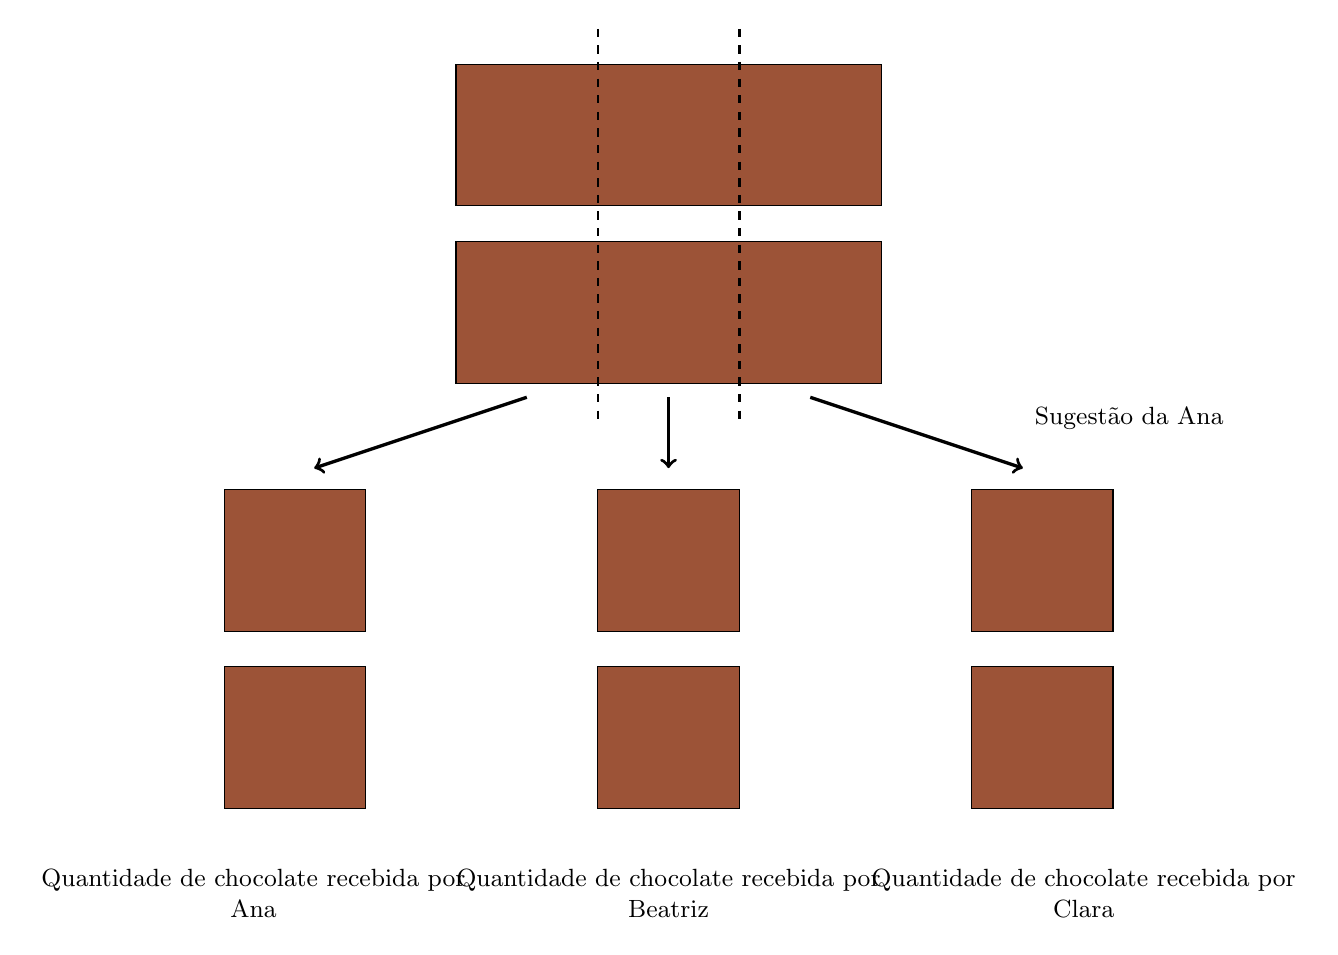
\begin{tikzpicture}[x=1mm,y=1mm,scale=0.9]
%%%%%%%%%% espaço entre um início de barra repartida e outro.
\def\hsp{150} 
%%%%%%%%%% barras de chocolate
\draw[fill=Sepia!60](0,10) rectangle (60,30);
\draw[fill=Sepia!60] (0,-15) rectangle (60,5);

%%%%%%%%% cortes
\draw[dashed, thick] (20,35) -- (20,-20);
\draw[dashed, thick] (40,35) -- (40,-20);

%%%%%%%%% setas
\draw[very thick, ->] (10,-17) -- (-20,-27);
\draw[very thick, ->] (30,-17) -- (30,-27);
\draw[very thick, ->] (50,-17) -- (80,-27);

\node at (95,-20) {\parbox[b]{30mm}{\centering  \small Sugestão da Ana}};

%%%%%%%%%%%%%%%%%%Pedaços repartidos  
\draw[fill=Sepia!60,xshift=-\hsp] (20,-50) rectangle (40,-30);
\draw[fill=Sepia!60,xshift=-\hsp] (20,-75) rectangle (40,-55);

\draw[fill=Sepia!60] (20,-50) rectangle (40,-30);
\draw[fill=Sepia!60] (20,-75) rectangle (40,-55);

\draw[fill=Sepia!60,xshift=\hsp] (20,-50) rectangle (40,-30);
\draw[fill=Sepia!60,xshift=\hsp] (20,-75) rectangle (40,-55);

%%%%%%%%% Texto embaixo
% \draw [thick, decoration={brace,mirror,raise=5}, decorate, xshift=-\hsp] (31.25,-2) -- (51.25,-2) node [pos=0.5,anchor=north,yshift=-10] {\parbox[b]{40mm}{\centering Quantidade de chocolate recebida por Ana}};

\node [xshift=-\hsp] at (30,-87) {\parbox[b]{55mm}{\centering \small Quantidade de chocolate recebida por Ana}};

\node at (30,-87) {\parbox[b]{55mm}{\centering  \small Quantidade de chocolate recebida por Beatriz}};

\node  [xshift=\hsp] at (30,-87) {\parbox[b]{55mm}{\centering  \small Quantidade de chocolate recebida por Clara}};

%%%%%%%%%%%% Balões em volta
% \draw [dotted, xshift=-\hsp] (30,-52.5) ellipse (20mm and 30mm);
% \draw [dotted] (30,-52.5) ellipse (20mm and 30mm);
% \draw [dotted, xshift=\hsp] (30,-52.5) ellipse (20mm and 30mm);
\end{tikzpicture}
\end{center}

\begin{enumerate}[a)] %s
  \item Na divisão de cada uma das barras de chocolate em três partes iguais, cada parte é que fração de uma barra de chocolate?
  \item Você concorda com a divisão que Ana sugeriu? Explique.
  \item Com essa divisão, as três irmãs receberam a mesma quantidade de chocolate?
  \item Na divisão proposta por Ana, como você nomearia, usando fração de uma barra de chocolate, a quantidade de chocolate que cada irmã recebeu?
\end{enumerate}

Ana não quer o chocolate e decidiu dar a quantidade de chocolate que recebeu na divisão das barras para as suas irmãs.

\begin{enumerate}[e)]
\item Se Ana desse metade da quantidade de chocolate que recebeu para cada uma de suas irmãs, que quantidade de chocolate Beatriz e Clara passariam a ter? Como você nomearia, usando frações, essas quantidades?
\item[f)] E se Ana desse toda a quantidade de chocolate que recebeu para Beatriz, que quantidade de chocolate  Beatriz passaria a ter? Como você nomearia, usando frações, essa quantidade?
\end{enumerate} %s
\end{atividade}

\begin{atividade}{}

Um grupo de cinco amigos (Amarildo, Beto, Carlos, Davi e Edilson) encomendou três tortas salgadas, de mesmo tamanho retangular, como na ilustração para uma comemoração.

\begin{center}
 \begin{tikzpicture}[scale=0.6]
  \draw (0,0) rectangle (60,30);
  \draw (70,0) rectangle (130,30);
  \draw (140,0) rectangle (200,30);
 \end{tikzpicture}

\end{center}

\begin{enumerate} [\quad a)] %s
  \item     Como dividir as três tortas de modo que cada amigo receba a mesma quantidade de torta? Faça um desenho no seu caderno mostrando sua proposta de divisão. Indique qual parte é de qual amigo!
  \item     Considerando-se uma torta como unidade, como você nomearia, usando frações, a quantidade de torta que:
\begin{enumerate} [\quad I)] %d
      \item         Amarildo recebeu?
      \item         Amarildo e Beto receberam juntos?
      \item         Amarildo, Beto e Carlos receberam juntos?
      \item         Amarildo, Beto, Carlos e Davi receberam juntos?
      \item         Amarildo, Beto, Carlos, Davi e Edilson receberam juntos?
\end{enumerate} %d

  \item     A quantidade de torta que cada amigo recebeu é menor do que um quinto de torta? E do que dois quintos de torta? Explique sua resposta.
  \item     A quantidade de torta que cada amigo recebeu é maior do que três quintos de torta? E do que quatro quintos de torta? Explique sua resposta.
\end{enumerate} %s
\end{atividade}

\begin{atividade}{}

Para a sobremesa do almoço de domingo, papai passou em uma confeitaria que vende tortas.
Cada torta está dividida em  igualmente em 8 fatias, como na figura abaixo.

\begin{center}
\includegraphics[width=.6\textwidth, keepaspectratio]{licao02/ativ3_fig01.png}
\end{center}

\begin{enumerate} [\quad a)] %s
  \item     Que fração de uma torta é uma fatia? Explique.
  \item     Domingo papai comprou 4 fatias, quantos oitavos de uma torta havia para a sobremesa?
  \item     Na pergunta anterior, apresente outra fração que represente a quantidade de torta que papai comprou. Explique sua resposta.
  \item     Hoje papai comprou 10 fatias de torta. Como podemos representar essa quantidade de torta em termos de frações de uma torta?
\end{enumerate} %s
\end{atividade}

\begin{atividade}{}

Complete as afirmações com uma das frações: ``dois meios'', ``dois terços'', ``dois quintos'', ``dois nonos'', ``três quartos'', ``seis oitavos'', ``oito sextos'' e ``nove meios'', para que sejam verdadeiras.

\begin{enumerate}[a)]
\item A parte pintada de vermelho em
     \begin{tikzpicture}[scale=0.8]
     \draw[fill=attention] (0,0) rectangle (20,10);
     \draw[] (10,0) -- (10,10);
     \draw[fill=common, fill opacity=.3] (20,0) rectangle (30,10);
     \end{tikzpicture}
     é
     \begin{tikzpicture}
     \draw (0,0) -- (20,0);
     \end{tikzpicture}
     de \begin{tikzpicture}[scale=0.8]
     \draw[fill=common, fill opacity=.3] (0,0) rectangle (30,10);
                               \end{tikzpicture}.
\item A parte pintada de vermelho em \begin{tikzpicture}
                           \draw[fill=attention] (0,0) rectangle (8,8);
                           \draw (0,0) -- (8,8);
                          \end{tikzpicture}
                          é \begin{tikzpicture}
                             \draw (0,0) -- (20,0);
                            \end{tikzpicture}
                            de \begin{tikzpicture}
                            \draw[fill=common, fill opacity=.3] (0,0) rectangle (8,8);
                           \end{tikzpicture}.


 \item A parte pintada de vermelho em \begin{tikzpicture}
                           \draw[fill=common, fill opacity=.3] (0,0) circle (4);
                           \fill[attention] (0,0) -- (72:4) arc (72:-72:4) --cycle;
                           \foreach \x in {0,72,...,288}{
                           \draw (0,0) -- (\x:4);}
                          \end{tikzpicture}
                          é \begin{tikzpicture}
                             \draw (0,0) -- (20,0);
                            \end{tikzpicture}
                            de \begin{tikzpicture}
                            \draw[fill=common, fill opacity=.3] (0,0) circle (4);
                           \end{tikzpicture}.

 \item A parte pintada de vermelho em \begin{tikzpicture}
                                       \fill[attention]  \foreach \x/\y in {36/72,108/144,180/212, 252/284, 324/360}{ (0,0) -- (\x-18:4) -- (\y-18:2)--(\x-18 +72:4) -- (0, 0)};
                                       \draw  \foreach \x/\y in {36/72,108/144,180/212, 252/284, 324/360}{ (\x-18:4) -- (\y-18:2)--(\x-18 +72:4)};
                                      \end{tikzpicture} \begin{tikzpicture}
                                       \fill[attention]  \foreach \x/\y in {36/72,108/144,180/212, 252/284, 324/360}{ (0,0) -- (\x-18:4) -- (\y-18:2)--(\x-18 +72:4) -- (0, 0)};
                                       \draw  \foreach \x/\y in {36/72,108/144,180/212, 252/284, 324/360}{ (\x-18:4) -- (\y-18:2)--(\x-18 +72:4)};
                                      \end{tikzpicture} \begin{tikzpicture}
                                       \fill[attention]  \foreach \x/\y in {36/72,108/144,180/212, 252/284, 324/360}{ (0,0) -- (\x-18:4) -- (\y-18:2)--(\x-18 +72:4) -- (0, 0)};
                                       \draw  \foreach \x/\y in {36/72,108/144,180/212, 252/284, 324/360}{ (\x-18:4) -- (\y-18:2)--(\x-18 +72:4)};
                                      \end{tikzpicture} \begin{tikzpicture}
                                       \fill[attention]  \foreach \x/\y in {36/72,108/144,180/212, 252/284, 324/360}{ (0,0) -- (\x-18:4) -- (\y-18:2)--(\x-18 +72:4) -- (0, 0)};
                                       \draw  \foreach \x/\y in {36/72,108/144,180/212, 252/284, 324/360}{ (\x-18:4) -- (\y-18:2)--(\x-18 +72:4)};
                                      \end{tikzpicture} \begin{tikzpicture}
                                       \fill[attention]  \foreach \x/\y in {36/72,108/144,180/212, 252/284, 324/360}{ (0,0) -- (\x-18:4) -- (\y-18:2)--(\x-18 +72:4) -- (0, 0)};
                                       \fill[white]  (90:4) -- (-90:2) -- (-56:4) -- (-18:2)-- (18:4) --(56:2) --cycle;
                                       \fill[common, opacity=.3]  (90:4) -- (-90:2) -- (-56:4) -- (-18:2)-- (18:4) --(56:2) --cycle;
                                       \draw  \foreach \x/\y in {36/72,108/144,180/212, 252/284, 324/360}{ (\x-18:4) -- (\y-18:2)--(\x-18 +72:4)};
                                      \end{tikzpicture} é \begin{tikzpicture} \draw (0,0) -- (20,0); \end{tikzpicture} de \begin{tikzpicture}
                                       \fill[common, opacity=.3]  \foreach \x/\y in {36/72,108/144,180/212, 252/284, 324/360}{ (0,0) -- (\x-18:4) -- (\y-18:2)--(\x-18 +72:4) -- (0, 0)};
                                       \draw  \foreach \x/\y in {36/72,108/144,180/212, 252/284, 324/360}{ (\x-18:4) -- (\y-18:2)--(\x-18 +72:4)};
                                      \end{tikzpicture}.

\item A parte pintada de vermelho em \begin{tikzpicture} \draw[fill=attention] (90:4)--(-90:4)--(-30:4)--(30:4)--cycle; \foreach \x in {30,90,...,330}{\draw (0,0) -- (\x:4);} \draw[fill=common, fill opacity=.3] (90:4) -- (150:4) -- (210:4) -- (270:4) -- cycle;\end{tikzpicture} \begin{tikzpicture} \fill[attention] (30:4)--(90:4)--(150:4)--(210:4)--(270:4)-- (330:4) -- (0,0) --cycle; \foreach \x in {30,90,...,330}{\draw (0,0) -- (\x:4); \draw (\x:4) -- (\x+60:4);} \fill[common, fill opacity=.3] (0,0) -- (30:4) -- (-30:4) -- cycle;\end{tikzpicture} é \begin{tikzpicture} \draw (0,0) -- (20,0); \end{tikzpicture} de \begin{tikzpicture} \draw[fill=common, fill opacity=.3] (30:4) --(90:4)--(150:4)--(210:4)--(270:4)-- (330:4) -- cycle;\end{tikzpicture}.
\end{enumerate}
\end{atividade}

\section{ORGANIZANDO AS IDEIAS }

Se uma torta está dividida em três partes iguais, a torta fica separada em três terços. Assim,  como visto na historinha do início da lição, tanto faz escrever ``um terço da torta'' ou, usando símbolos matemáticos, ``$\frac{1}{3}$ da torta'' para se referir à fatia destacada na figura.

\begin{center}
\begin{tikzpicture}
 \draw[fill=common, fill opacity=.3] (0,0) circle (10);
 \draw[fill=attention] (0,0) -- (-90:10) arc (-90:30:10) -- (0,0) -- cycle;
 \draw (0,0) -- (-90:10);
 \draw (0,0) -- (30:10);
 \draw (0,0) -- (150:10);
 \node at (0,-14) {$\frac{1}{3}$ da torta};
 \node at (0,-20) {(lê-se: ``um terço da torta'')};
\end{tikzpicture}
\end{center}


Duas fatias são ``dois terços da torta'', o que pode ser expresso usando símbolos matemáticos por ``$\frac{2}{3}$ da torta''. Deste modo, ``três terços da torta'' é uma torta inteira.

\begin{center}
\begin{tikzpicture}
 \draw[fill=common, fill opacity=.3] (0,0) circle (10);
 \draw[fill=attention] (0,0) -- (-210:10) arc (-210:30:10) -- (0,0) -- cycle;
 \draw (0,0) circle (10);
 \draw (0,0) -- (-90:10);
 \draw (0,0) -- (30:10);
 \draw (0,0) -- (150:10);
 \node at (0,-14) {$\frac{2}{3}$ da torta};
  \node at (0,-20) {(lê-se: ``dois terços da torta'')};
\end{tikzpicture}\quad \quad \quad \begin{tikzpicture}
 \draw[fill=attention] (0,0) circle (10);
 \draw (0,0) -- (-90:10);
 \draw (0,0) -- (30:10);
 \draw (0,0) -- (150:10);
 \node at (0,-14) {$\frac{3}{3}$ da torta = 1 torta};
 \node at (0,-20) {(lê-se: ``três terços da torta'' ou ``uma torta'')};
\end{tikzpicture}
\end{center}


Também pode-se considerar quatro terços, cinco terços ou seis terços da torta, basta juntar novos terços à torta inteira.

\begin{center}
\begin{tikzpicture}
\begin{scope}[shift={(-24,0)}]
 \draw[fill=attention] (0,0) circle (10);
 \draw (0,0) -- (-90:10);
 \draw (0,0) -- (30:10);
 \draw (0,0) -- (150:10);
 \end{scope}
 \draw[fill=common, fill opacity=.3] (0,0) circle (10);
 \draw[fill=attention] (0,0) -- (150:10) arc (150:30:10) -- (0,0) -- cycle;
 \draw (0,0) -- (270:10);
 \node at (-12,-14) {$\frac{4}{3}$ da torta = 1 torta e $\frac{1}{3}$ da torta};
  \node at (-12,-20) {(lê-se: ``quatro terços da torta'' ou ``uma torta e um terço de torta'')};
\end{tikzpicture}
\vspace{0.4cm}

\begin{tikzpicture}
\begin{scope}[shift={(-24,0)}]
 \draw[fill=attention] (0,0) circle (10);
 \draw (0,0) -- (-90:10);
 \draw (0,0) -- (30:10);
 \draw (0,0) -- (150:10);
\end{scope}
 \draw[fill=common, fill opacity=.3] (0,0) circle (10);
 \draw[fill=attention] (0,0) -- (150:10) arc (150:-90:10) -- (0,0) -- cycle;
 \draw (0,0) -- (30:10);
 \node at (-12,-14) {$\frac{5}{3}$ da torta = 1 torta e $\frac{2}{3}$ da torta};
   \node at (-12,-20) {(lê-se: ``cinco terços da torta'' ou ``uma torta e dois terços da torta'')};
\end{tikzpicture}
\vspace{0.4cm}

\begin{tikzpicture}
\begin{scope}[shift={(-24,0)}]
 \draw[fill=attention] (0,0) circle (10);
 \draw (0,0) -- (-90:10);
 \draw (0,0) -- (30:10);
 \draw (0,0) -- (150:10);
 \end{scope}
 \draw[fill=attention] (0,0) circle (10);
 \draw (0,0) -- (-90:10);
 \draw (0,0) -- (30:10);
 \draw (0,0) -- (150:10);
 \node at (-12,-14) {$\frac{6}{3}$ da torta = 2 tortas};
   \node at (-12,-20) {(lê-se: ``seis terços da torta'' ou ``duas tortas'')};
\end{tikzpicture}
\end{center}

%Se uma torta é repartida em três partes iguais, cada fatia é ``um terço da torta''. Juntando-se uma dessas fatias por vez obtém-se dois terços e três terços da torta. Com mais do que uma torta repartidas cada uma em três partes iguais, pode-se obter quatro terços, cinco terços, seis terços de torta e assim por diante.

Nos exemplos anteriores, todas as frações são lidas com ``terços'' pois as tortas foram repartidas em três partes iguais. \textbf{Usando símbolos matemáticos, as frações são escritas com dois números e um traço.} Por exemplo, em ``$\frac{2}{3}$ da torta'', o ``3'' nomeia a fração ``terço'' e, por isso, é chamado \textit{denominador da fração} $\frac{2}{3}$. O número ``2'' indica a quantidade de terços que estão sendo considerados e é chamado \textit{numerador da fração} $\frac{2}{3}$. Isso acontece em todas as frações:

\begin{center}
  % \includegraphics[width=.9\textwidth, keepaspectratio]{licao02/orgideias_fig01.png}
  \includegraphics[width=.9\textwidth, keepaspectratio]{licao02/orgideias_fig01b.png}
\end{center}

\begin{itemize}
\item Em $\frac{2}{5}$, por exemplo, o numerador é 2 e o denominador é 5. Lê-se {\it dois quintos}.
\item Em $\frac{10}{8}$, por exemplo, o numerador é 10 e o denominador é 8. Lê-se {\it dez oitavos}.
\end{itemize}


Para ler a fração deve-se ler o {\bf número} do numerador seguido do {\bf nome que identifica as partes em que foi repartida a unidade, que é indicado pelo denominador}, nessa ordem. Veja:

\begin{center}
\begin{tabular}[c]{lclcl}
  $\dfrac{1}{3}\rightarrow$ um terço;& \quad & $\dfrac{2}{3}\rightarrow$ dois terços; & \quad & $\dfrac{5}{3}\rightarrow$ cinco terços; \\
  \\
$\dfrac{1}{8}\rightarrow$ um oitavo;& \quad & $\dfrac{3}{8}\rightarrow$ três oitavos; & \quad & $\dfrac{7}{8}\rightarrow$ sete oitavos.  
\end{tabular}
\end{center}

Anote agora os nomes de algumas outras frações:

\begin{center}
  \begin{tabular}[c]{lclcl}
    $\dfrac{1}{2}\rightarrow$  um meio; & \quad & $\dfrac{1}{3}\rightarrow$   um terço; & \quad &  $\dfrac{1}{4}\rightarrow$ um quarto;\\
    \\
    $\dfrac{1}{5}\rightarrow$   um quinto; & \quad &  $\dfrac{1}{6}\rightarrow$  um sexto; & \quad & $\dfrac{1}{7}\rightarrow$  um sétimo;\\
    \\
$\dfrac{1}{8}\rightarrow$   um oitavo; & \quad & $\dfrac{1}{9}\rightarrow$  um nono; & \quad & $\dfrac{1}{10}\rightarrow$   um décimo.
  \end{tabular}
\end{center}

Já a fração $\frac{1}{11}$ não é chamada ``um décimo primeiro''.
Na leitura de frações com denominadores maiores do que 10, utiliza-se a palavra avos.
Assim, a fração $\frac{1}{11}$ é lida ``um onze avos''.
Veja outros exemplos:  
$$\frac{1}{12}\rightarrow \text{  um doze avos;}\quad \frac{1}{13}\rightarrow \text{ um treze avos;} \quad \frac{5}{13}\rightarrow \text{ cinco treze avos.}$$

%Curioso para saber sobre o significado da palavra {\bf avos}?
%Pergunte ao seu professor.
%O importante é lembrar que, para denominadores maiores 10, acrescenta-se a expressão ``avos'' ao final da leitura da fração. %Não se esqueça que

Na leitura das frações cujos denominadores são 100, 1000, 1000, etc. não se usa ``avos''. Observe: 
$$\frac{1}{100}\rightarrow \text{ um centésimo;}\quad \frac{13}{100} \rightarrow \text{treze centésimos;} \quad
\frac{33}{1000}\rightarrow \text{ trinta e três milésimos.}$$

{\bf Pronto! Agora você já é capaz de ler diversos tipos de frações.}

\section{MÃO NA MASSA }


\begin{atividade}{}

Uma pizza gigante foi dividida em doze fatias iguais.
Pedro comeu quatro fatias, Isabella cinco fatias, Bernardo duas fatias e Manuela apenas uma fatia.

\begin{center}
  \begin{tabular}{|m{0.27\textwidth}|m{0.13\textwidth}|m{0.13\textwidth}|m{0.13\textwidth}|m{0.13\textwidth}|}
\hline
& \centering Pedro & \centering  Isabella & \centering  Bernardo &  \quad Manuela  \\
    \hline  \hline
   Pinte a fração de pizza consumida  por cada pessoa      & \parbox[c][2cm]{0.13\textwidth}{\centering 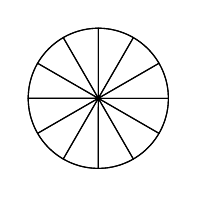
\begin{tikzpicture}[x=1.0cm,y=1.0cm, scale=0.5]
\draw (1.76,2.04) circle (1.78cm);
\draw [shift={(1.76,2.04)}]  (0,0) --  plot[domain=0.:0.5235987755982987,variable=\t]({1.*1.78*cos(\t r)+0.*1.78*sin(\t r)},{0.*1.78*cos(\t r)+1.*1.78*sin(\t r)}) -- cycle ;
\draw [shift={(1.76,2.04)}]  (0,0) --  plot[domain=0.5235987755982987:1.0471975511965974,variable=\t]({1.*1.78*cos(\t r)+0.*1.78*sin(\t r)},{0.*1.78*cos(\t r)+1.*1.78*sin(\t r)}) -- cycle ;
\draw [shift={(1.76,2.04)}]  (0,0) --  plot[domain=1.0471975511965974:1.5707963267948963,variable=\t]({1.*1.78*cos(\t r)+0.*1.78*sin(\t r)},{0.*1.78*cos(\t r)+1.*1.78*sin(\t r)}) -- cycle ;
\draw [shift={(1.76,2.04)}]  (0,0) --  plot[domain=1.5707963267948963:2.0943951023931953,variable=\t]({1.*1.78*cos(\t r)+0.*1.78*sin(\t r)},{0.*1.78*cos(\t r)+1.*1.78*sin(\t r)}) -- cycle ;
\draw [shift={(1.76,2.04)}]  (0,0) --  plot[domain=2.0943951023931953:2.617993877991494,variable=\t]({1.*1.78*cos(\t r)+0.*1.78*sin(\t r)},{0.*1.78*cos(\t r)+1.*1.78*sin(\t r)}) -- cycle ;
\draw [shift={(1.76,2.04)}]  (0,0) --  plot[domain=2.617993877991494:3.1415926535897927,variable=\t]({1.*1.78*cos(\t r)+0.*1.78*sin(\t r)},{0.*1.78*cos(\t r)+1.*1.78*sin(\t r)}) -- cycle ;
\draw [shift={(1.76,2.04)}]  (0,0) --  plot[domain=3.1415926535897927:3.6651914291880914,variable=\t]({1.*1.78*cos(\t r)+0.*1.78*sin(\t r)},{0.*1.78*cos(\t r)+1.*1.78*sin(\t r)}) -- cycle ;
\draw [shift={(1.76,2.04)}]  (0,0) --  plot[domain=3.6651914291880914:4.18879020478639,variable=\t]({1.*1.78*cos(\t r)+0.*1.78*sin(\t r)},{0.*1.78*cos(\t r)+1.*1.78*sin(\t r)}) -- cycle ;
\draw [shift={(1.76,2.04)}]  (0,0) --  plot[domain=4.18879020478639:4.712388980384689,variable=\t]({1.*1.78*cos(\t r)+0.*1.78*sin(\t r)},{0.*1.78*cos(\t r)+1.*1.78*sin(\t r)}) -- cycle ;
\draw [shift={(1.76,2.04)}]  (0,0) --  plot[domain=4.712388980384689:5.235987755982988,variable=\t]({1.*1.78*cos(\t r)+0.*1.78*sin(\t r)},{0.*1.78*cos(\t r)+1.*1.78*sin(\t r)}) -- cycle ;
\draw [shift={(1.76,2.04)}]  (0,0) --  plot[domain=5.235987755982988:5.759586531581286,variable=\t]({1.*1.78*cos(\t r)+0.*1.78*sin(\t r)},{0.*1.78*cos(\t r)+1.*1.78*sin(\t r)}) -- cycle ;
\draw [shift={(1.76,2.04)}]  (0,0) --  plot[domain=-0.5235987755983:0.,variable=\t]({1.*1.78*cos(\t r)+0.*1.78*sin(\t r)},{0.*1.78*cos(\t r)+1.*1.78*sin(\t r)}) -- cycle ;
\end{tikzpicture}}
  & \parbox[c][2cm]{0.13\textwidth}{\centering 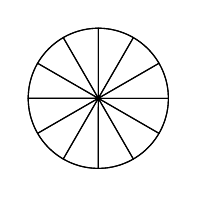
\begin{tikzpicture}[x=1.0cm,y=1.0cm, scale=0.5]
\draw (1.76,2.04) circle (1.78cm);
\draw [shift={(1.76,2.04)}]  (0,0) --  plot[domain=0.:0.5235987755982987,variable=\t]({1.*1.78*cos(\t r)+0.*1.78*sin(\t r)},{0.*1.78*cos(\t r)+1.*1.78*sin(\t r)}) -- cycle ;
\draw [shift={(1.76,2.04)}]  (0,0) --  plot[domain=0.5235987755982987:1.0471975511965974,variable=\t]({1.*1.78*cos(\t r)+0.*1.78*sin(\t r)},{0.*1.78*cos(\t r)+1.*1.78*sin(\t r)}) -- cycle ;
\draw [shift={(1.76,2.04)}]  (0,0) --  plot[domain=1.0471975511965974:1.5707963267948963,variable=\t]({1.*1.78*cos(\t r)+0.*1.78*sin(\t r)},{0.*1.78*cos(\t r)+1.*1.78*sin(\t r)}) -- cycle ;
\draw [shift={(1.76,2.04)}]  (0,0) --  plot[domain=1.5707963267948963:2.0943951023931953,variable=\t]({1.*1.78*cos(\t r)+0.*1.78*sin(\t r)},{0.*1.78*cos(\t r)+1.*1.78*sin(\t r)}) -- cycle ;
\draw [shift={(1.76,2.04)}]  (0,0) --  plot[domain=2.0943951023931953:2.617993877991494,variable=\t]({1.*1.78*cos(\t r)+0.*1.78*sin(\t r)},{0.*1.78*cos(\t r)+1.*1.78*sin(\t r)}) -- cycle ;
\draw [shift={(1.76,2.04)}]  (0,0) --  plot[domain=2.617993877991494:3.1415926535897927,variable=\t]({1.*1.78*cos(\t r)+0.*1.78*sin(\t r)},{0.*1.78*cos(\t r)+1.*1.78*sin(\t r)}) -- cycle ;
\draw [shift={(1.76,2.04)}]  (0,0) --  plot[domain=3.1415926535897927:3.6651914291880914,variable=\t]({1.*1.78*cos(\t r)+0.*1.78*sin(\t r)},{0.*1.78*cos(\t r)+1.*1.78*sin(\t r)}) -- cycle ;
\draw [shift={(1.76,2.04)}]  (0,0) --  plot[domain=3.6651914291880914:4.18879020478639,variable=\t]({1.*1.78*cos(\t r)+0.*1.78*sin(\t r)},{0.*1.78*cos(\t r)+1.*1.78*sin(\t r)}) -- cycle ;
\draw [shift={(1.76,2.04)}]  (0,0) --  plot[domain=4.18879020478639:4.712388980384689,variable=\t]({1.*1.78*cos(\t r)+0.*1.78*sin(\t r)},{0.*1.78*cos(\t r)+1.*1.78*sin(\t r)}) -- cycle ;
\draw [shift={(1.76,2.04)}]  (0,0) --  plot[domain=4.712388980384689:5.235987755982988,variable=\t]({1.*1.78*cos(\t r)+0.*1.78*sin(\t r)},{0.*1.78*cos(\t r)+1.*1.78*sin(\t r)}) -- cycle ;
\draw [shift={(1.76,2.04)}]  (0,0) --  plot[domain=5.235987755982988:5.759586531581286,variable=\t]({1.*1.78*cos(\t r)+0.*1.78*sin(\t r)},{0.*1.78*cos(\t r)+1.*1.78*sin(\t r)}) -- cycle ;
\draw [shift={(1.76,2.04)}]  (0,0) --  plot[domain=-0.5235987755983:0.,variable=\t]({1.*1.78*cos(\t r)+0.*1.78*sin(\t r)},{0.*1.78*cos(\t r)+1.*1.78*sin(\t r)}) -- cycle ;
\end{tikzpicture}}
   & \parbox[c][2cm]{0.13\textwidth}{\centering 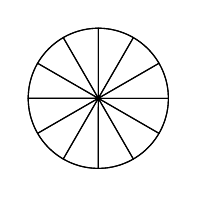
\begin{tikzpicture}[x=1.0cm,y=1.0cm, scale=0.5]
\draw (1.76,2.04) circle (1.78cm);
\draw [shift={(1.76,2.04)}]  (0,0) --  plot[domain=0.:0.5235987755982987,variable=\t]({1.*1.78*cos(\t r)+0.*1.78*sin(\t r)},{0.*1.78*cos(\t r)+1.*1.78*sin(\t r)}) -- cycle ;
\draw [shift={(1.76,2.04)}]  (0,0) --  plot[domain=0.5235987755982987:1.0471975511965974,variable=\t]({1.*1.78*cos(\t r)+0.*1.78*sin(\t r)},{0.*1.78*cos(\t r)+1.*1.78*sin(\t r)}) -- cycle ;
\draw [shift={(1.76,2.04)}]  (0,0) --  plot[domain=1.0471975511965974:1.5707963267948963,variable=\t]({1.*1.78*cos(\t r)+0.*1.78*sin(\t r)},{0.*1.78*cos(\t r)+1.*1.78*sin(\t r)}) -- cycle ;
\draw [shift={(1.76,2.04)}]  (0,0) --  plot[domain=1.5707963267948963:2.0943951023931953,variable=\t]({1.*1.78*cos(\t r)+0.*1.78*sin(\t r)},{0.*1.78*cos(\t r)+1.*1.78*sin(\t r)}) -- cycle ;
\draw [shift={(1.76,2.04)}]  (0,0) --  plot[domain=2.0943951023931953:2.617993877991494,variable=\t]({1.*1.78*cos(\t r)+0.*1.78*sin(\t r)},{0.*1.78*cos(\t r)+1.*1.78*sin(\t r)}) -- cycle ;
\draw [shift={(1.76,2.04)}]  (0,0) --  plot[domain=2.617993877991494:3.1415926535897927,variable=\t]({1.*1.78*cos(\t r)+0.*1.78*sin(\t r)},{0.*1.78*cos(\t r)+1.*1.78*sin(\t r)}) -- cycle ;
\draw [shift={(1.76,2.04)}]  (0,0) --  plot[domain=3.1415926535897927:3.6651914291880914,variable=\t]({1.*1.78*cos(\t r)+0.*1.78*sin(\t r)},{0.*1.78*cos(\t r)+1.*1.78*sin(\t r)}) -- cycle ;
\draw [shift={(1.76,2.04)}]  (0,0) --  plot[domain=3.6651914291880914:4.18879020478639,variable=\t]({1.*1.78*cos(\t r)+0.*1.78*sin(\t r)},{0.*1.78*cos(\t r)+1.*1.78*sin(\t r)}) -- cycle ;
\draw [shift={(1.76,2.04)}]  (0,0) --  plot[domain=4.18879020478639:4.712388980384689,variable=\t]({1.*1.78*cos(\t r)+0.*1.78*sin(\t r)},{0.*1.78*cos(\t r)+1.*1.78*sin(\t r)}) -- cycle ;
\draw [shift={(1.76,2.04)}]  (0,0) --  plot[domain=4.712388980384689:5.235987755982988,variable=\t]({1.*1.78*cos(\t r)+0.*1.78*sin(\t r)},{0.*1.78*cos(\t r)+1.*1.78*sin(\t r)}) -- cycle ;
\draw [shift={(1.76,2.04)}]  (0,0) --  plot[domain=5.235987755982988:5.759586531581286,variable=\t]({1.*1.78*cos(\t r)+0.*1.78*sin(\t r)},{0.*1.78*cos(\t r)+1.*1.78*sin(\t r)}) -- cycle ;
\draw [shift={(1.76,2.04)}]  (0,0) --  plot[domain=-0.5235987755983:0.,variable=\t]({1.*1.78*cos(\t r)+0.*1.78*sin(\t r)},{0.*1.78*cos(\t r)+1.*1.78*sin(\t r)}) -- cycle ;
\end{tikzpicture}}
  & \parbox[c][2cm]{0.13\textwidth}{\centering 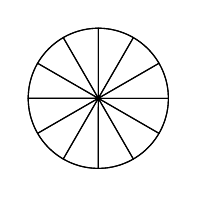
\begin{tikzpicture}[x=1.0cm,y=1.0cm, scale=0.5]
\draw (1.76,2.04) circle (1.78cm);
\draw [shift={(1.76,2.04)}]  (0,0) --  plot[domain=0.:0.5235987755982987,variable=\t]({1.*1.78*cos(\t r)+0.*1.78*sin(\t r)},{0.*1.78*cos(\t r)+1.*1.78*sin(\t r)}) -- cycle ;
\draw [shift={(1.76,2.04)}]  (0,0) --  plot[domain=0.5235987755982987:1.0471975511965974,variable=\t]({1.*1.78*cos(\t r)+0.*1.78*sin(\t r)},{0.*1.78*cos(\t r)+1.*1.78*sin(\t r)}) -- cycle ;
\draw [shift={(1.76,2.04)}]  (0,0) --  plot[domain=1.0471975511965974:1.5707963267948963,variable=\t]({1.*1.78*cos(\t r)+0.*1.78*sin(\t r)},{0.*1.78*cos(\t r)+1.*1.78*sin(\t r)}) -- cycle ;
\draw [shift={(1.76,2.04)}]  (0,0) --  plot[domain=1.5707963267948963:2.0943951023931953,variable=\t]({1.*1.78*cos(\t r)+0.*1.78*sin(\t r)},{0.*1.78*cos(\t r)+1.*1.78*sin(\t r)}) -- cycle ;
\draw [shift={(1.76,2.04)}]  (0,0) --  plot[domain=2.0943951023931953:2.617993877991494,variable=\t]({1.*1.78*cos(\t r)+0.*1.78*sin(\t r)},{0.*1.78*cos(\t r)+1.*1.78*sin(\t r)}) -- cycle ;
\draw [shift={(1.76,2.04)}]  (0,0) --  plot[domain=2.617993877991494:3.1415926535897927,variable=\t]({1.*1.78*cos(\t r)+0.*1.78*sin(\t r)},{0.*1.78*cos(\t r)+1.*1.78*sin(\t r)}) -- cycle ;
\draw [shift={(1.76,2.04)}]  (0,0) --  plot[domain=3.1415926535897927:3.6651914291880914,variable=\t]({1.*1.78*cos(\t r)+0.*1.78*sin(\t r)},{0.*1.78*cos(\t r)+1.*1.78*sin(\t r)}) -- cycle ;
\draw [shift={(1.76,2.04)}]  (0,0) --  plot[domain=3.6651914291880914:4.18879020478639,variable=\t]({1.*1.78*cos(\t r)+0.*1.78*sin(\t r)},{0.*1.78*cos(\t r)+1.*1.78*sin(\t r)}) -- cycle ;
\draw [shift={(1.76,2.04)}]  (0,0) --  plot[domain=4.18879020478639:4.712388980384689,variable=\t]({1.*1.78*cos(\t r)+0.*1.78*sin(\t r)},{0.*1.78*cos(\t r)+1.*1.78*sin(\t r)}) -- cycle ;
\draw [shift={(1.76,2.04)}]  (0,0) --  plot[domain=4.712388980384689:5.235987755982988,variable=\t]({1.*1.78*cos(\t r)+0.*1.78*sin(\t r)},{0.*1.78*cos(\t r)+1.*1.78*sin(\t r)}) -- cycle ;
\draw [shift={(1.76,2.04)}]  (0,0) --  plot[domain=5.235987755982988:5.759586531581286,variable=\t]({1.*1.78*cos(\t r)+0.*1.78*sin(\t r)},{0.*1.78*cos(\t r)+1.*1.78*sin(\t r)}) -- cycle ;
\draw [shift={(1.76,2.04)}]  (0,0) --  plot[domain=-0.5235987755983:0.,variable=\t]({1.*1.78*cos(\t r)+0.*1.78*sin(\t r)},{0.*1.78*cos(\t r)+1.*1.78*sin(\t r)}) -- cycle ;
\end{tikzpicture}}
  \\
    \hline
     Escreva, por extenso, a fração de pizza consumida por cada pessoa&                                        &                                        &                                         &                                        \\
    \hline
     Escreva, usando símbolos matemáticos, a fração de pizza consumida por cada pessoa &                                        &                                        &                                         &                                        \\
    \hline
  \end{tabular}
\end{center}

\begin{enumerate} [\quad a)] %d
  \item Na sua opinião, qual maneira de representar fração ``gasta menos lápis'': pintando, escrevendo por extenso ou usando símbolos matemáticos?
  \item Na sua opinião, qual a representação que mais rapidamente ajuda a decidir quem comeu mais e quem comeu menos pizza?
\end{enumerate} %d
\end{atividade}

\begin{atividade}{}
Um grupo de amigos está dividindo duas pizzas circulares iguais, isto é, de mesmo tamanho. A primeira pizza foi cortada em 4 fatias de mesmo tamanho. A segunda pizza foi repartida em 8 pedaços iguais.
\begin{enumerate} [\quad a)] %s
\item Uma fatia da primeira pizza é que fração dessa pizza? Responda usando símbolos matemáticos.
\item Uma fatia da segunda pizza é que fração dessa pizza? Responda usando símbolos matemáticos.
\item Qual fatia tem mais quantidade de pizza: uma fatia da primeira ou uma fatia da segunda? Explique usando uma figura.
\end{enumerate} %s
\end{atividade}

\begin{atividade}{}
Para cada figura a seguir, indique a fração da figura que está pintada de vermelho. Esta fração é maior, menor ou exatamente igual a $\frac{1}{2}$ da figura?



\begin{enumerate}
\begin{multicols}{3}
\item
\adjustbox{valign=t}
{
\begin{tikzpicture}
\draw[fill=common, fill opacity=.3] (0,0) circle (10);
 \foreach \x in {0,72,...,288}{
 \draw[fill=attention] (0,0) -- (\x:10) arc (\x:\x+36:10) --cycle;
 \draw (\x:10) -- (\x:-10);}
\end{tikzpicture} 
}

\item
\adjustbox{valign=t}
{

\begin{tikzpicture}
\draw[fill=common, fill opacity=.3] (0,0) rectangle (14,20);
\draw[fill=attention] (0,4) rectangle (7,20);
\foreach \y in {4,8,12,16}{
\draw (0,\y)--(14,\y);}
\draw (7,0) -- (7,20);
\end{tikzpicture}
}


\item\adjustbox{valign=t}
{

\begin{tikzpicture}
\draw[fill=common, fill opacity=.3] (0,0) rectangle (30,20);
\fill[attention] (0,0) rectangle (18,20);
 \foreach \x in {3,6,...,27}{
 \draw (\x,0)--(\x,20);}
\end{tikzpicture} 
}

\end{multicols}
\end{enumerate}

\end{atividade}

\begin{atividade}{}

Na tabela a seguir, pinte cada figura de modo que a parte pintada seja a fração da figura indicada na coluna à esquerda e na mesma linha. Indique também, usando símbolos matemáticos, qual fração da figura ficou sem ser pintada.

\begin{center}
  \begin{longtable}{|m{0.25\textwidth}|m{0.2\textwidth}|m{0.25\textwidth}|}
    \hline
      Fração da figura que deve ser pintada  & \centering  Figura  &   Fração da figura que ficou sem ser pintada  \\
    \hline \hline
    \endhead
     \centering $\dfrac{5}{6}$  & \centering \parbox[c][1.75cm][c]{1.6cm}{\begin{tikzpicture}
                                    \foreach \x in {0,60,...,300}{ \draw (0,0)--(\x:8);\draw (\x:8)--(\x+60:8);}
                                   \end{tikzpicture}}
&  \\
    \hline
     \centering $\dfrac{3}{4}$  &  \centering \parbox[c][1.75cm][c]{1.6cm}{\begin{tikzpicture}
                                    \draw (0:8)--(180:8);
                                    \draw (90:8)--(270:8);
                                    \draw (0,0) circle (8);
                                   \end{tikzpicture}}
                                   &  \\
    \hline
     \centering $\dfrac{2}{5}$  &   \centering \parbox[c][1.75cm][c]{2.4cm}{
                                    \begin{tikzpicture}
                                    \draw (0,0) rectangle (25,16);
                                    \foreach \x in {5,10,15,20}{\draw (\x,0)--(\x,16);}
                                   \end{tikzpicture} }
                                   &  \\
    \hline
     \centering $\dfrac{2}{3}$  &  \centering \parbox[c][1.75cm][c]{1.6cm}{\begin{tikzpicture}
                                    \foreach \x in {0,60,...,300}{ \draw (0,0)--(\x:8);\draw (\x:8)--(\x+60:8);}
                                   \end{tikzpicture}}
                                   &  \\
    \hline
     \centering $\dfrac{3}{8}$  &   \centering \parbox[c][1.75cm][c]{1.6cm}{\begin{tikzpicture}
                                    \draw (0:8)--(180:8);
                                    \draw (90:8)--(270:8);
                                    \draw (0,0) circle (8);
                                   \end{tikzpicture}}&  \\
    \hline
     \centering $\dfrac{9}{10}$  & \centering \parbox[c][1.75cm][c]{2.4cm}{
                                    \begin{tikzpicture}
                                    \draw (0,0) rectangle (25,16);
                                    \foreach \x in {5,10,15,20}{\draw (\x,0)--(\x,16);}
                                   \end{tikzpicture} }
                                   &  \\
    \hline
  \end{longtable}
\end{center}
\end{atividade}

\begin{atividade}{}
A figura mostra três copos idênticos.  É possível armazenar a água dos três copos em um único copo sem que transborde? Explique usando frações.

\begin{center}
\begin{tikzpicture}[scale=0.3, x=1cm,y=1cm]

% Definição do eixo vertical das elipses
\def\EixoM{0.5}

% colorindo o primeiro cilindro
\fill[common] (2,0) ellipse (2 and \EixoM);
\fill[common] (0,0) rectangle (4,3);
\fill[common] (2,3) ellipse (2 and \EixoM);

% colorindo o segundo cilindro
\fill[common] (8,0) ellipse (2 and \EixoM);
\fill[common] (6,0) rectangle (10,2);
\fill[common] (8,2) ellipse (2 and \EixoM);

% colorindo o terceiro
\fill[common] (14,0) ellipse (2 and \EixoM);
\fill[common] (12,0) rectangle (16,4);
\fill[common] (14,4) ellipse (2 and \EixoM);

% shift horizontal nos cilindros definido por \x
\foreach \x in {0,6,12}{
\draw (\x,0)--(\x,8);
\draw (\x + 4,0)--(\x + 4,8);
% shift vertical nos arcos de elipse definido por \y
\foreach \y in {0,1,...,7}{
\pgfpathmoveto{\pgfpoint{\x cm}{\y cm}}
\pgfpatharc{-180}{0}{2cm and \EixoM cm}
\pgfusepath{draw}}
\draw (\x + 2,8) ellipse (2 and \EixoM);}

\node at (2,-2) {(1)};
\node at (8,-2) {(2)};
\node at (14,-2) {(3)};
\end{tikzpicture}

\end{center}
\end{atividade}

\clearpage
\begin{atividade}{}

\begin{center}
  \begin{longtable}{|m{0.2\textwidth}|m{0.2\textwidth}|m{0.5\textwidth}|}
    \hline
     \centering Fração da unidade  & \centering  Figura correspondente à fração da unidade  & \quad \quad \quad Desenhe aqui a unidade  \\
    \hline \hline
    \endhead
     \centering $\dfrac{1}{2}$  &\centering \parbox[c][1.1cm]{1.5cm}{\begin{tikzpicture}
                                    \draw[fill=common, fill opacity=.3] (0,0) rectangle (12,6);
                                   \end{tikzpicture}}
 &  \\
    \hline
     \centering $\dfrac{4}{2}$  &   \centering \parbox[c][1.1cm]{1.5cm}{\begin{tikzpicture}
                                    \draw[fill=common, fill opacity=.3] (0,0) rectangle (12,6);
                                   \end{tikzpicture}}
                                   &  \\
    \hline
     \centering $\dfrac{3}{2}$  &  \centering \parbox[c][1.1cm]{1.5cm}{\begin{tikzpicture}
                                    \draw[fill=common, fill opacity=.3] (0,0) rectangle (12,6);
                                   \end{tikzpicture}}
                                   &  \\
    \hline
     \centering $\dfrac{2}{3}$  &  \centering \parbox[c][1.1cm]{1.5cm}{\begin{tikzpicture}
                                    \draw[fill=common, fill opacity=.3] (0,0) rectangle (12,6);
                                   \end{tikzpicture}}
                                   &  \\
    \hline
     \centering $\dfrac{1}{2}$  &  \centering \parbox[c][1.1cm]{1.5cm}{\begin{tikzpicture}
                                    \draw[fill=common, fill opacity=.3] (0,0) arc (0:180:6) -- cycle;
                                   \end{tikzpicture}}  &  \\
    \hline
      \centering $\dfrac{4}{2}$  &  \centering \parbox[c][1.1cm]{1.5cm}{\begin{tikzpicture}
                                    \draw[fill=common, fill opacity=.3] (0,0) arc (0:180:6) -- cycle;
                                   \end{tikzpicture}} &  \\
    \hline
      \centering $\dfrac{3}{2}$  &  \centering \parbox[c][1.1cm]{1.5cm}{\begin{tikzpicture}
                                    \draw[fill=common, fill opacity=.3] (0,0) arc (0:180:6) -- cycle;
                                   \end{tikzpicture}}  &  \\
    \hline
      \centering $\dfrac{2}{3}$  &  \centering \parbox[c][1.1cm]{1.5cm}{\begin{tikzpicture}
                                    \draw[fill=common, fill opacity=.3] (0,0) arc (0:180:6) -- cycle;
                                   \end{tikzpicture}} &  \\
    \hline
      \centering $\dfrac{1}{2}$  &  \centering \parbox[c][1.1cm]{1.5cm}{\begin{tikzpicture}
                                    \draw[fill=common, fill opacity=.3] (0,0) rectangle (12,1);
                                   \end{tikzpicture}}  &  \\
    \hline
      \centering $\dfrac{4}{2}$  &  \centering \parbox[c][1.1cm]{1.5cm}{\begin{tikzpicture}
                                    \draw[fill=common, fill opacity=.3] (0,0) rectangle (12,1);
                                   \end{tikzpicture}}  &  \\
    \hline
      \centering $\dfrac{3}{2}$  &  \centering \parbox[c][1.1cm]{1.5cm}{\begin{tikzpicture}
                                    \draw[fill=common, fill opacity=.3] (0,0) rectangle (12,1);
                                   \end{tikzpicture}}  &  \\
    \hline
      \centering $\dfrac{2}{3}$  &  \centering \parbox[c][1.1cm]{1.5cm}{\begin{tikzpicture}
                                    \draw[fill=common, fill opacity=.3] (0,0) rectangle (12,1);
                                   \end{tikzpicture}}   &  \\
    \hline
        \centering $\dfrac{1}{2}$  &  \centering \parbox[c][1.1cm]{1.5cm}{ \begin{tikzpicture}
                                      \draw[fill=common, fill opacity=.3] (0:4) -- (60:4)--(120:4)-- (180:4)--(240:4)--(300:4)--cycle;
                                     \end{tikzpicture} } &  \\
     \hline
     \centering $\dfrac{4}{2}$  &  \centering \parbox[c][1.1cm]{1.5cm}{ \begin{tikzpicture}
                                    \draw[fill=common, fill opacity=.3] (0:4) -- (60:4)--(120:4)-- (180:4)--(240:4)--(300:4)--cycle;
                                   \end{tikzpicture} } &  \\
     \hline
       \centering $\dfrac{3}{2}$  &  \centering \parbox[c][1.1cm]{1.5cm}{ \begin{tikzpicture}
                                    \draw[fill=common, fill opacity=.3] (0:4) -- (60:4)--(120:4)-- (180:4)--(240:4)--(300:4)--cycle;
                                   \end{tikzpicture} } &  \\
    \hline
      \centering $\dfrac{2}{3}$  &  \centering \parbox[c][1.1cm]{1.5cm}{ \begin{tikzpicture}
                                    \draw[fill=common, fill opacity=.3] (0:4) -- (60:4)--(120:4)-- (180:4)--(240:4)--(300:4)--cycle;
                                   \end{tikzpicture} } &  \\
    \hline
  \end{longtable}
\end{center}
\end{atividade}

\begin{atividade}{}

Lucas, Matheus, Heitor, Rafael, Enzo, Nicolas, Lorenzo, Guilherme e Samuel estavam brincando de empurrar seus carrinhos de brinquedo para ver qual carrinho ia mais longe em uma pista reta.

A figura a seguir mostra o quão longe foi o carrinho de Lucas e onde ele parou na pista com relação ao ponto de largada.

\begin{center}
\includegraphics[width=450pt, keepaspectratio]{licao02/ativ12_fig01.png}
\end{center}

Sabe-se que:

\begin{enumerate} [\quad a)] %s
  \item     O carrinho de Matheus só conseguiu ir até a metade da distância percorrida pelo carrinho de Lucas.
  \item     O carrinho de Heitor conseguiu ir até     $\frac{3}{2}$     da distância percorrida pelo carrinho de Lucas.
  \item     O carrinho de Rafael conseguiu ir até     $\frac{4}{2}$     da distância percorrida pelo carrinho de Lucas.
  \item     O carrinho de Enzo conseguiu ir até     $\frac{5}{2}$     da distância percorrida pelo carrinho de Lucas.
  \item     O carrinho de Nicolas conseguiu ir até     $\frac{6}{2}$     da distância percorrida pelo carrinho de Lucas.
  \item     O carrinho de Lorenzo conseguiu ir até     $\frac{6}{4}$     da distância percorrida pelo carrinho de Lucas.
  \item     O carrinho de Guilherme conseguiu ir até o dobro da distância percorrida pelo carrinho de Lucas.
  \item     O carrinho de Samuel conseguiu ir até     $\frac{6}{3}$     da distância percorrida pelo carrinho de Lucas.
\end{enumerate} %s


Com essas informações, marque as posições de parada dos carrinhos de todos os amigos de Lucas no encarte que você irá receber.

\begin{center}
\includegraphics[width=450pt, keepaspectratio]{licao02/ativ12_fig01.png}
\end{center}


Os carrinhos de Rafael e Samuel pararam no mesmo lugar? Explique.
\end{atividade}

\begin{atividade}{}

Anita, Gustavo e Henrique descobriram que todos tinham levado bolo para o lanche.\newline
Anita falou: ``Mamãe colocou metade do bolo no meu lanche.''\newline
Gustavo falou: ``Eu trouxe um terço do bolo que minha tia fez.''\newline
Henrique falou: ``Eu trouxe apenas um quinto do bolo que minha mãe preparou!''\newline
Para surpresa de todos, ao retirarem seus lanches da mochila, descobriram que todos traziam-no em  embalagens iguais, portanto traziam a mesma quantidade de bolo.\newline
Como você explica tal situação?
\end{atividade}

\section{QUEBRANDO A CUCA }
\vspace*{-.4cm}


\begin{atividade}{}

(NAEP, 1992) Pense cuidadosamente nesta questão. Escreva uma resposta completa. Você pode usar desenhos, palavras e números para explicar sua resposta. Certifique-se de mostrar todo o seu raciocínio.

José comeu $\frac{1}{2}$ de uma pizza. Ella comeu $\frac{1}{2}$ de uma outra pizza. José disse que ele comeu mais pizza do que Ella, mas Ella diz que eles comeram a mesma quantidade. Use palavras, figuras ou números para mostrar que José pode estar certo.
%\vspace*{-.5cm}
\end{atividade}

\begin{atividade}{}

Complete as sentenças a seguir com uma fração adequada (usando símbolos matemáticos). Perceba que uma mesma região pintada pode ser descrita por frações diferentes, dependendo da unidade considerada.

%definição da região limitada pelos 2 hexágonos encaixados.
\def \tripinha{ (30:4) -- (90:4) -- (150:4)--(210:4)--(270:4)--(330:4) [shift={({4*sqrt(3)},0)}] --(270:4) -- (330:4) -- (30:4) -- (90:4)--(150:4)--cycle;}
%definição da região limitada pelos 3 hexágonos encaixados.
\def \tripa{ (30:4) -- (90:4) -- (150:4)--(210:4)--(270:4)--(330:4) [shift={({4*sqrt(3)},0)}] --(270:4) -- (330:4) [shift={({4*sqrt(3)},0)}]--  (270:4) -- (330:4) -- (30:4) -- (90:4)--(150:4) [shift={({-4*sqrt(3)},0)}] -- (90:4) -- (150:4)--cycle;}

\begin{enumerate} [\quad a)] %s
%a
\item     A região pintada em vermelho em
\begin{tikzpicture}[scale=1.3]
 \draw \tripa;
\begin{scope}
 \clip \tripa;
\draw[fill=attention] (-4,-4) rectangle (0,4);
\draw[fill=common, fill opacity=.3] (0,-4) rectangle (20,4);
\end{scope}
\end{tikzpicture}
é
\begin{tikzpicture} \draw (0,0)--(20,0);\end{tikzpicture}
de
\begin{tikzpicture}[scale=1.3]
\draw[fill=common, fill opacity=.3] (30:4) -- (90:4) -- (150:4) -- (210:4) -- (270:4) -- (330:4)--cycle;
\end{tikzpicture}.
 %b
\item     A região pintada em vermelho em
\begin{tikzpicture}[scale=1.3]
 \draw \tripa;
\begin{scope}
 \clip \tripa;
\draw[fill=attention] (-4,-4) rectangle (0,4);
\draw[fill=common, fill opacity=.3] (0,-4) rectangle (20,4);
\end{scope}
\end{tikzpicture}
é
\begin{tikzpicture} \draw (0,0)--(20,0);\end{tikzpicture}
de
\begin{tikzpicture}[scale=1.3]
 \draw[fill=common, fill opacity=.3] (30:4) -- (90:4) -- (150:4)--(210:4)--(270:4)--(330:4) [shift={({4*sqrt(3)},0)}] --(270:4) -- (330:4) --(30:4) -- (90:4) -- (150:4)--cycle;
\end{tikzpicture}.

%c
\item     A região pintada em vermelho em \begin{tikzpicture}[scale=1.3]
 \draw \tripa;
\begin{scope}
 \clip \tripa;
\draw[fill=attention] (-4,-4) rectangle (0,4);
\draw[fill=common, fill opacity=.3] (0,-4) rectangle (20,4);
\end{scope}
\end{tikzpicture}
     é \begin{tikzpicture} \draw (0,0)--(20,0);\end{tikzpicture}    de
\begin{tikzpicture}[scale=1.3]
\draw[fill=common, fill opacity=.3] \tripa;
\end{tikzpicture}.

%d
 \item     A região pintada em vermelho em  \begin{tikzpicture}[scale=1.3]
 \draw \tripa;
\begin{scope}
 \clip \tripa;
\draw[fill=attention] (-4,-4) rectangle ({4*sqrt(3)},4);
\draw[fill=common, fill opacity=.3] ({4*sqrt(3)},-4) rectangle ({10*sqrt(3)},4);
\end{scope}
\end{tikzpicture}  é \begin{tikzpicture} \draw (0,0)--(20,0);\end{tikzpicture}    de
\begin{tikzpicture}[scale=1.3]
\draw[fill=common, fill opacity=.3] (30:4) -- (90:4) -- (150:4) -- (210:4) -- (270:4) -- (330:4)--cycle;
\end{tikzpicture}.
%e
\item     A região pintada em vermelho em   \begin{tikzpicture}[scale=1.3]
 \draw \tripa;
\begin{scope}
 \clip \tripa;
\draw[fill=attention] (-4,-4) rectangle ({4*sqrt(3)},4);
\draw[fill=common, fill opacity=.3] ({4*sqrt(3)},-4) rectangle ({10*sqrt(3)},4);
\end{scope}
\end{tikzpicture}    é \begin{tikzpicture} \draw (0,0)--(20,0);\end{tikzpicture}    de
\begin{tikzpicture}[scale=1.3]
 \draw[fill=common, fill opacity=.3] (30:4) -- (90:4) -- (150:4)--(210:4)--(270:4)--(330:4) [shift={({4*sqrt(3)},0)}] --(270:4) -- (330:4) --(30:4) -- (90:4) -- (150:4)--cycle;
\end{tikzpicture}.

%f
\item     A região pintada em vermelho em  \begin{tikzpicture}[scale=1.3]
 \draw \tripa;
\begin{scope}
 \clip \tripa;
\draw[fill=attention] (-4,-4) rectangle ({4*sqrt(3)},4);
\draw[fill=common, fill opacity=.3] ({4*sqrt(3)},-4) rectangle ({10*sqrt(3)},4);
\end{scope}
\end{tikzpicture}   é \begin{tikzpicture} \draw (0,0)--(20,0);\end{tikzpicture}    de
\begin{tikzpicture}[scale=1.3]
\draw[fill=common, fill opacity=.3] \tripa;
\end{tikzpicture}.

%g
\item     A região pintada em vermelho em
\begin{tikzpicture}[scale=1.3]
 \draw \tripa;
\begin{scope}
 \clip \tripa;
\draw[fill=attention] (-4,-4) rectangle ({8*sqrt(3)},4);
\draw[fill=common, fill opacity=.3] ({8*sqrt(3)},-4) rectangle ({10*sqrt(3)},4);
\end{scope}
\end{tikzpicture}
é \begin{tikzpicture} \draw (0,0)--(20,0);\end{tikzpicture}    de
\begin{tikzpicture}[scale=1.3]
\draw[fill=common, fill opacity=.3] (30:4) -- (90:4) -- (150:4) -- (210:4) -- (270:4) -- (330:4)--cycle;
\end{tikzpicture}.
%h
\item     A região pintada em vermelho em  \begin{tikzpicture}[scale=1.3]
 \draw \tripa;
\begin{scope}
 \clip \tripa;
\draw[fill=attention] (-4,-4) rectangle ({8*sqrt(3)},4);
\draw[fill=common, fill opacity=.3] ({8*sqrt(3)},-4) rectangle ({10*sqrt(3)},4);
\end{scope}
\end{tikzpicture} é \begin{tikzpicture} \draw (0,0)--(20,0);\end{tikzpicture}    de
\begin{tikzpicture}[scale=1.3]
 \draw[fill=common, fill opacity=.3] (30:4) -- (90:4) -- (150:4)--(210:4)--(270:4)--(330:4) [shift={({4*sqrt(3)},0)}] --(270:4) -- (330:4) --(30:4) -- (90:4) -- (150:4)--cycle;
\end{tikzpicture}.

%i
\item     A região pintada em vermelho em
\begin{tikzpicture}[scale=1.3]
 \draw \tripa;
\begin{scope}
 \clip \tripa;
\draw[fill=attention] (-4,-4) rectangle ({8*sqrt(3)},4);
\draw[fill=common, fill opacity=.3] ({8*sqrt(3)},-4) rectangle ({10*sqrt(3)},4);
\end{scope}
\end{tikzpicture}
é \begin{tikzpicture} \draw (0,0)--(20,0);\end{tikzpicture}    de
\begin{tikzpicture}[scale=1.3]
\draw[fill=common, fill opacity=.3] \tripa;
\end{tikzpicture}.
%j
\item     A região pintada em vermelho em
  \begin{tikzpicture}[scale=1.3]
 \draw \tripa;
\begin{scope}
 \clip \tripa;
\draw[fill=attention] (-4,-4) rectangle ({12*sqrt(3)},4);
\end{scope}
\end{tikzpicture}
é \begin{tikzpicture} \draw (0,0)--(20,0);\end{tikzpicture}    de
\begin{tikzpicture}[scale=1.3]
\draw[fill=common, fill opacity=.3] (30:4) -- (90:4) -- (150:4) -- (210:4) -- (270:4) -- (330:4)--cycle;
\end{tikzpicture}.
%k
\item     A região pintada em vermelho em
\begin{tikzpicture}[scale=1.3]
 \draw \tripa;
\begin{scope}
 \clip \tripa;
\draw[fill=attention] (-4,-4) rectangle ({12*sqrt(3)},4);
\end{scope}
\end{tikzpicture}
é \begin{tikzpicture} \draw (0,0)--(20,0);\end{tikzpicture}    de
\begin{tikzpicture}[scale=1.3]
 \draw[fill=common, fill opacity=.3] (30:4) -- (90:4) -- (150:4)--(210:4)--(270:4)--(330:4) [shift={({4*sqrt(3)},0)}] --(270:4) -- (330:4) --(30:4) -- (90:4) -- (150:4)--cycle;
\end{tikzpicture}.

%l
\item     A região pintada em vermelho em
  \begin{tikzpicture}[scale=1.3]
 \draw \tripa;
\begin{scope}
 \clip \tripa;
\draw[fill=attention] (-4,-4) rectangle ({12*sqrt(3)},4);
\end{scope}
\end{tikzpicture}
é \begin{tikzpicture} \draw (0,0)--(20,0);\end{tikzpicture}    de
\begin{tikzpicture}[scale=1.3]
\draw[fill=common, fill opacity=.3] \tripa;
\end{tikzpicture}.

\end{enumerate} %s
\end{atividade}

\begin{atividade}{}

Miguel disse para Alice que a parte pintada de vermelho na figura a seguir corresponde a $\frac{3}{5}$ da figura, pois ela está dividida em 5 partes e 3 partes estão pintadas. Você concorda com a afirmação e com a justificativa de Miguel? Explique!

\begin{center}
\begin{tikzpicture}[scale=1.5]
%\fill[fill=attention,fill opacity=0.1] (0.,5.) -- (9.,5.) -- (9.,-5.) -- (0.,-5.) -- cycle;
\filldraw[fill=attention,fill opacity=1.0] (0,0) rectangle (9,5);
\filldraw[fill=common, fill opacity=.3] (0,-5) rectangle (9,0);
%\draw   (0.,5.)-- (9.,5.);
%\draw   (9.,5.)-- (9.,-5.);

%\draw   (0.,-5.)-- (0.,5.);
%\draw   (0.,5.)-- (0.,0.);
%\draw   (0.,0.)-- (9.,0.);
%\draw   (9.,0.)-- (9.,5.);
%\draw   (9.,5.)-- (0.,5.);
%\draw   (0.,5.)-- (9.,5.);
%\draw   (9.,0.)-- (0.,0.);
%\draw   (0.,0.)-- (0.,5.);
%\draw   (9.,5.)-- (9.,0.);
\draw   (3.,0.)-- (3.,5.);
\draw   (6.,5.)-- (6.,0.);
\draw   (4.5,-5.)-- (4.5,0.);
\draw   (0.,-5.)-- (9.,-5.);
%\draw   (9.,-5.)-- (9.,0.);
%\draw   (9.,0.)-- (0.,0.);
%\draw   (0.,0.)-- (0.,-5.);
% \begin{scriptsize}
% %\draw[color=ffqqqq] (4.725943121127749,2.6736730506884316) node {$pol2$};
% \end{scriptsize}
\draw   (9.,-5.)-- (0.,-5.);
\end{tikzpicture}
\end{center}
\end{atividade}
%\vspace*{-.6cm}


\begin{atividade}{}

A figura a seguir tem 3 partes pintadas de vermelho e 4 partes pintadas de azul. É correto afirmar que a parte pintada de vermelho corresponde a $\frac{3}{4}$ da figura? Explique.
\begin{center}
\begin{tikzpicture}[scale=3.5]%[line cap=round,line join=round,>=triangle 45,x=1.0cm,y=1.0cm]
\fill[fill=attention] (0.,3.) -- (3.,3.) -- (3.,0.) -- (0.,0.) -- cycle;
\fill[common, fill opacity=.3] (3,0) rectangle (7,3);
\draw (1.,3.)-- (1.,0.);
\draw (2.,0.)-- (2.,3.);
\draw (3.,3.)-- (3.,0.);
\draw (4.,0.)-- (4.,3.);
\draw (5.,3.)-- (5.,0.);
\draw (6.,0.)-- (6.,3.);
\draw (7.,3.)-- (7.,0.);
\draw (0.,3.)-- (7.,3.);
\draw (7.,3.)-- (7.,0.);
\draw (7.,0.)-- (0.,0.);
\draw (0.,0.)-- (0.,3.);
\end{tikzpicture}
\end{center}
\end{atividade}

\begin{atividade}{}

\begin{enumerate} [\quad a)] %s
  \item     A região em vermelho na figura a seguir representa $\frac{1}{2}$ ou $\frac{1}{4}$?
\begin{center}
\begin{tikzpicture}[scale=1.5]
 \draw \tripinha;
\begin{scope}
 \clip \tripinha;
\draw[fill=attention] (-4,-4) rectangle (0,4);
\draw[fill=common, fill opacity=.3] (0,-4) rectangle (12,4);
\end{scope}
\end{tikzpicture}
\end{center}

  \item     A região em vermelho na figura a seguir representa     $\frac{1}{2}$     ou     $\frac{3}{2}$?
\begin{center}
\begin{tikzpicture}[scale=1.5]
 \draw \tripa;
\begin{scope}
 \clip \tripa;
\draw[fill=attention] (-4,-4) rectangle ({4*sqrt(3)},4);
\draw[fill=common, fill opacity=.3] ({4*sqrt(3)},-4) rectangle ({12*sqrt(3)},4);
\end{scope}
\end{tikzpicture}
\end{center}
\def \tripalonga{ (30:4) -- (90:4) -- (150:4)--(210:4)--(270:4)--(330:4) [shift={({4*sqrt(3)},0)}] --(270:4) -- (330:4) [shift={({4*sqrt(3)},0)}] --(270:4) -- (330:4)[shift={({4*sqrt(3)},0)}] --(270:4) -- (330:4) [shift={({4*sqrt(3)},0)}]--  (270:4) -- (330:4) -- (30:4) -- (90:4)--(150:4) [shift={({-4*sqrt(3)},0)}] -- (90:4) -- (150:4)[shift={({-4*sqrt(3)},0)}] -- (90:4) -- (150:4) [shift={({-4*sqrt(3)},0)}] -- (90:4) -- (150:4)--cycle;}

  \item     A região em vermelho na figura a seguir representa     $\frac{3}{5}$     ou     $3$?
\begin{center}
\begin{tikzpicture}[scale=1.5]
 \draw \tripalonga;
\begin{scope}
 \clip \tripalonga;
  \draw[fill=attention] (-4,-4) rectangle ({10*sqrt(3)},4);
\draw[fill=common, fill opacity=.3] ({10*sqrt(3)},-4) rectangle ({20*sqrt(3)},4);
\end{scope}
\end{tikzpicture}
\end{center}

  \end{enumerate} %s

\end{atividade}

\begin{atividade}{}

Júlia, Davi e Laura estavam estudando a figura a seguir.
\begin{center}
\begin{tikzpicture}[scale=4]
%\fill(1.,3.) -- (6.,3.) -- (6.,0.02) -- (1.,0.) -- cycle;
\fill[attention] (1.,3.) -- (4.,3.) -- (4.,0.012) -- (1.,0.) -- cycle;
\fill[common, fill opacity=.3] (4,0) rectangle (6,3);
%\fill[line width=0.pt,color=black,fill=black,fill opacity=1.0] (4.,3.) -- (4.,0.012) -- (6.,0.04) -- (6.,3.) -- cycle;
\draw (1.,3.)-- (1.,0.);
\draw (2.,0.)-- (2.,3.);
\draw (3.,3.)-- (3.,0.);
\draw (4.,0.)-- (4.,3.);
\draw (5.,3.)-- (5.,0.);
\draw (6.,0.)-- (6.,3.);
\draw (1.,3.)-- (6.,3.);
\draw (6.,3.)-- (6.,0.02);
\draw (6.,0.02)-- (1.,0.);
\draw (1.,0.)-- (1.,3.);
\end{tikzpicture}
\end{center}
Júlia disse: ``A parte em vermelho representa $\frac{3}{5}$.''. Davi retrucou: ``Não, não! A parte em vermelho representa $\frac{3}{2}$!''. Laura, então acrescentou: ``Eu acho que a parte em vermelho representa $3$!''. Quem está certo? Júlia, Davi ou Laura? Explique!
\end{atividade}

\begin{atividade}{}

Em uma pizzaria rodízio, 7 amigos comem, ao todo, 38 fatias.

\begin{center}
\includegraphics[width=300pt, keepaspectratio]{licao02/ativ18_fig01.png}
\end{center}


Sabendo que nessa pizzaria cada pizza é repartida em 8 fatias de mesmo tamanho, pergunta-se:
\begin{enumerate} [\quad a)] %s
  \item     Quantas pizzas inteiras comeram os 7 amigos?
  \item     Que fração de uma pizza comeram  ao todo os amigos?
  \item     É possível que todos os amigos tenham comido o mesmo número de fatias de pizza? Explique.
\end{enumerate} %s
\end{atividade}


%%% Local Variables: 
%%% mode: latex
%%% TeX-master: "livro_aluno_completo.tex"
%%% End: 

% 

% 
% \mbox{}
% \thispagestyle{empty}
% \newpage

\setcounter{chapter}{2}
\chapter{Frações na reta numérica }
\setcounter{subsection}{0}
\section{EXPLORANDO O ASSUNTO }

\begin{atividade}{}

Os quadrinhos a seguir mostram uma caixa-d'água sendo enchida.
Para saber que fração da capacidade da caixa-d'água já está com água, será usada uma faixa graduada para indicar o nível de água na caixa.

\begin{table}[H]
\centering
\setlength\tabulinesep{10pt}
\begin{tabu} to \textwidth{|c|c|}
\hline

\begin{tikzpicture}[scale=2.5, x=1cm, y=1cm]



\draw [fill=brown] (-.3,0,0) -- (1.3,0,0) -- (1.3,0,1) -- (-.3,0,1) -- cycle;
\draw [fill=brown!70!black] (1.3,0,-0) -- (1.3,-.05,0) -- (1.3,-.05,1) -- (1.3,0,1);
\draw [fill=brown!70!black] (1.3,0,1) -- (1.3,-.05,1) -- (-.3,-.05,1) -- (-.3,0,1);



\draw (0,0,0) -- (1,0,0) -- (1,0,1) -- (0,0,1) -- cycle;

\draw (0,0,0) -- (0,1,0);
\draw [fill=white, opacity=.7] (0,1,0) -- (1,1,0) -- (1,1,1) -- (0,1,1) -- cycle;
\draw [fill=white, opacity=.7] (0,0,1) -- (1,0,1) -- (1,1,1) -- (0,1,1) -- cycle;

\fill [common!80] (0,.25,0) -- (1,.25,0) -- (1,.25,1) -- (0,.25,1) -- cycle;
\fill [common] (0,0,1) -- (1,0,1) -- (1,.25,1) -- (0,.25,1) -- cycle;
\fill [common] (1,0,0) -- (1,0,1) -- (1,.25,1) -- (1,.25,0) -- cycle;

\draw (1,0,1) -- (1,1,1);
\draw (1,0,0) -- (1,1,0);
\draw (0,0,1) -- (0,1,1);
\draw (1,0,0) -- (1,0,1) -- (0,0,1);

\node at (0.5,-.5,.5) {Momento 1};
\end{tikzpicture}

& 

\begin{tikzpicture}[scale=2.5, x=1cm, y=1cm]

\draw [fill=brown] (-.3,0,0) -- (1.3,0,0) -- (1.3,0,1) -- (-.3,0,1) -- cycle;
\draw [fill=brown!70!black] (1.3,0,-0) -- (1.3,-.05,0) -- (1.3,-.05,1) -- (1.3,0,1);
\draw [fill=brown!70!black] (1.3,0,1) -- (1.3,-.05,1) -- (-.3,-.05,1) -- (-.3,0,1);



\draw (0,0,0) -- (1,0,0) -- (1,0,1) -- (0,0,1) -- cycle;

\draw (0,0,0) -- (0,1,0);
\draw [fill=white, opacity=.7] (0,1,0) -- (1,1,0) -- (1,1,1) -- (0,1,1) -- cycle;
\draw [fill=white, opacity=.7] (0,0,1) -- (1,0,1) -- (1,1,1) -- (0,1,1) -- cycle;

\fill [common!80] (0,.5,0) -- (1,.5,0) -- (1,.5,1) -- (0,.5,1) -- cycle;
\fill [common] (0,0,1) -- (1,0,1) -- (1,.5,1) -- (0,.5,1) -- cycle;
\fill [common] (1,0,0) -- (1,0,1) -- (1,.5,1) -- (1,.5,0) -- cycle;

\draw (1,0,1) -- (1,1,1);
\draw (1,0,0) -- (1,1,0);
\draw (0,0,1) -- (0,1,1);
\draw (1,0,0) -- (1,0,1) -- (0,0,1);
\draw (0,1,0) -- (1,1,0) -- (1,1,1) -- (0,1,1) -- cycle;

\node at (0.5,-.5,.5) {Momento 2};
\end{tikzpicture} \\

\hline

\begin{tikzpicture}[scale=2.5, x=1cm, y=1cm]

\draw [fill=brown] (-.3,0,0) -- (1.3,0,0) -- (1.3,0,1) -- (-.3,0,1) -- cycle;
\draw [fill=brown!70!black] (1.3,0,-0) -- (1.3,-.05,0) -- (1.3,-.05,1) -- (1.3,0,1);
\draw [fill=brown!70!black] (1.3,0,1) -- (1.3,-.05,1) -- (-.3,-.05,1) -- (-.3,0,1);



\draw (0,0,0) -- (1,0,0) -- (1,0,1) -- (0,0,1) -- cycle;

\draw (0,0,0) -- (0,1,0);
\draw [fill=white, opacity=.7] (0,1,0) -- (1,1,0) -- (1,1,1) -- (0,1,1) -- cycle;
\draw [fill=white, opacity=.7] (0,0,1) -- (1,0,1) -- (1,1,1) -- (0,1,1) -- cycle;

\fill [common!80] (0,.75,0) -- (1,.75,0) -- (1,.75,1) -- (0,.75,1) -- cycle;
\fill [common] (0,0,1) -- (1,0,1) -- (1,.75,1) -- (0,.75,1) -- cycle;
\fill [common] (1,0,0) -- (1,0,1) -- (1,.75,1) -- (1,.75,0) -- cycle;

\draw (1,0,1) -- (1,1,1);
\draw (1,0,0) -- (1,1,0);
\draw (0,0,1) -- (0,1,1);
\draw (1,0,0) -- (1,0,1) -- (0,0,1);
\draw (0,1,0) -- (1,1,0) -- (1,1,1) -- (0,1,1) -- cycle;

\node at (0.5,-.5,.5) {Momento 3};
\end{tikzpicture}

& 
\begin{tikzpicture}[scale=2.5, x=1cm, y=1cm]

\draw [fill=brown] (-.3,0,0) -- (1.3,0,0) -- (1.3,0,1) -- (-.3,0,1) -- cycle;
\draw [fill=brown!70!black] (1.3,0,-0) -- (1.3,-.05,0) -- (1.3,-.05,1) -- (1.3,0,1);
\draw [fill=brown!70!black] (1.3,0,1) -- (1.3,-.05,1) -- (-.3,-.05,1) -- (-.3,0,1);



\draw (0,0,0) -- (1,0,0) -- (1,0,1) -- (0,0,1) -- cycle;

\draw (0,0,0) -- (0,1,0);
\draw [fill=white, opacity=.7] (0,1,0) -- (1,1,0) -- (1,1,1) -- (0,1,1) -- cycle;
\draw [fill=white, opacity=.7] (0,0,1) -- (1,0,1) -- (1,1,1) -- (0,1,1) -- cycle;


\fill [common!80] (0,1,0) -- (1,1,0) -- (1,1,1) -- (0,1,1) -- cycle;
\fill [common] (0,0,1) -- (1,0,1) -- (1,1,1) -- (0,1,1) -- cycle;
\fill [common] (1,0,0) -- (1,0,1) -- (1,1,1) -- (1,1,0) -- cycle;

\draw (1,0,1) -- (1,1,1);
\draw (1,0,0) -- (1,1,0);
\draw (0,0,1) -- (0,1,1);
\draw (1,0,0) -- (1,0,1) -- (0,0,1);
\draw (0,1,0) -- (1,1,0) -- (1,1,1) -- (0,1,1) -- cycle;


\node at (0.5,-.5,.5) {Momento 4};
\end{tikzpicture} \\
\hline
\end{tabu}
\end{table}

Escolha, para cada um dos momentos, a graduação que lhe parece mais adequada para registrar a quantidade de água representada em cada uma das imagens. Explique sua escolha.

\begin{enumerate}
\begin{multicols}{2}

\item\adjustbox{valign=t}{
\begin{tikzpicture}[scale=2.5, x=1cm, y=1cm]

\draw [fill=brown] (-.3,0,0) -- (1.3,0,0) -- (1.3,0,1) -- (-.3,0,1) -- cycle;
\draw [fill=brown!70!black] (1.3,0,-0) -- (1.3,-.05,0) -- (1.3,-.05,1) -- (1.3,0,1);
\draw [fill=brown!70!black] (1.3,0,1) -- (1.3,-.05,1) -- (-.3,-.05,1) -- (-.3,0,1);

\draw [fill=white, opacity=.7] (0,0,0) -- (1,0,0) -- (1,0,1) -- (0,0,1) -- cycle;
\draw [fill=white, opacity=.7] (0,0,0) -- (0,1,0) -- (1,1,0) -- (1,0,0) -- cycle;
\draw [fill=white, opacity=.7] (0,0,0) -- (0,1,0) -- (0,1,1) -- (0,0,1) -- cycle;
\draw [fill=white, opacity=.7] (0,0,1) -- (1,0,1) -- (1,1,1) -- (0,1,1) -- cycle;
\draw [fill=white, opacity=.7] (1,0,0) -- (1,0,1) -- (1,1,1) -- (1,1,0) -- cycle;
\draw [fill=white, opacity=.7] (0,1,0) -- (1,1,0) -- (1,1,1) -- (0,1,1) -- cycle;

\filldraw [fill=white] (0,-.05,1) rectangle (0.3,1.05,1);
\draw [|-|] (.1,0,1) -- (.1,1,1) node [right, scale=.75, xshift=.05cm] {\footnotesize 1} node [ right, pos=0, scale=.75, xshift=.05cm]{\footnotesize 0};
\draw [|-|] (.1,0,1) -- (.1,.5,1) node [right, scale=.75, xshift=.025cm,pos=.5] {\footnotesize $\frac{1}{2}$};

\end{tikzpicture}  
}
\item\adjustbox{valign=t}{
\begin{tikzpicture}[scale=2.5, x=1cm, y=1cm]

\draw [fill=brown] (-.3,0,0) -- (1.3,0,0) -- (1.3,0,1) -- (-.3,0,1) -- cycle;
\draw [fill=brown!70!black] (1.3,0,-0) -- (1.3,-.05,0) -- (1.3,-.05,1) -- (1.3,0,1);
\draw [fill=brown!70!black] (1.3,0,1) -- (1.3,-.05,1) -- (-.3,-.05,1) -- (-.3,0,1);



\draw [fill=white, opacity=.7] (0,0,0) -- (1,0,0) -- (1,0,1) -- (0,0,1) -- cycle;
\draw [fill=white, opacity=.7] (0,0,0) -- (0,1,0) -- (1,1,0) -- (1,0,0) -- cycle;
\draw [fill=white, opacity=.7] (0,0,0) -- (0,1,0) -- (0,1,1) -- (0,0,1) -- cycle;
\draw [fill=white, opacity=.7] (0,0,1) -- (1,0,1) -- (1,1,1) -- (0,1,1) -- cycle;
\draw [fill=white, opacity=.7] (1,0,0) -- (1,0,1) -- (1,1,1) -- (1,1,0) -- cycle;
\draw [fill=white, opacity=.7] (0,1,0) -- (1,1,0) -- (1,1,1) -- (0,1,1) -- cycle;

\filldraw [fill=white] (0,-.05,1) rectangle (0.3,1.05,1);
\draw [|-|] (.1,0,1) -- (.1,1,1) node [right, scale=.75, xshift=.05cm] {\footnotesize 1} node [ right, pos=0, scale=.75, xshift=.05cm]{\footnotesize 0};
\draw [|-|] (.1,0,1) -- (.1,.5,1) node [right, scale=.75, xshift=.025cm] {\footnotesize $\frac{1}{2}$};
\draw [|-|] (.1,0,1) -- (.1,.25,1) node [right, scale=.75, xshift=.025cm] {\footnotesize $\frac{1}{4}$};
\draw [|-|] (.1,0,1) -- (.1,.75,1) node [right, scale=.75, xshift=.025cm] { \footnotesize $\frac{3}{4}$};


\end{tikzpicture}  
}
\end{multicols}

\begin{multicols}{2}
\item\adjustbox{valign=t}{
\begin{tikzpicture}[scale=2.5, x=1cm, y=1cm]

\draw [fill=brown] (-.3,0,0) -- (1.3,0,0) -- (1.3,0,1) -- (-.3,0,1) -- cycle;
\draw [fill=brown!70!black] (1.3,0,-0) -- (1.3,-.05,0) -- (1.3,-.05,1) -- (1.3,0,1);
\draw [fill=brown!70!black] (1.3,0,1) -- (1.3,-.05,1) -- (-.3,-.05,1) -- (-.3,0,1);



\draw [fill=white, opacity=.7] (0,0,0) -- (1,0,0) -- (1,0,1) -- (0,0,1) -- cycle;
\draw [fill=white, opacity=.7] (0,0,0) -- (0,1,0) -- (1,1,0) -- (1,0,0) -- cycle;
\draw [fill=white, opacity=.7] (0,0,0) -- (0,1,0) -- (0,1,1) -- (0,0,1) -- cycle;
\draw [fill=white, opacity=.7] (0,0,1) -- (1,0,1) -- (1,1,1) -- (0,1,1) -- cycle;
\draw [fill=white, opacity=.7] (1,0,0) -- (1,0,1) -- (1,1,1) -- (1,1,0) -- cycle;
\draw [fill=white, opacity=.7] (0,1,0) -- (1,1,0) -- (1,1,1) -- (0,1,1) -- cycle;

\filldraw [fill=white] (0,-.05,1) rectangle (0.3,1.05,1);
\draw [|-|] (.1,0,1) -- (.1,1,1) node [right, scale=.75, xshift=.05cm] {\footnotesize 1} node [ right, pos=0, scale=.75, xshift=.05cm]{\footnotesize 0};

\draw [|-|] (.1,0,1) -- (.1,.75,1) node [right, scale=.75, xshift=.025cm] { \footnotesize $\frac{1}{2}$};  
\end{tikzpicture}
}


\item\adjustbox{valign=t}{
\begin{tikzpicture}[scale=2.5, x=1cm, y=1cm]

\draw [fill=brown] (-.3,0,0) -- (1.3,0,0) -- (1.3,0,1) -- (-.3,0,1) -- cycle;
\draw [fill=brown!70!black] (1.3,0,-0) -- (1.3,-.05,0) -- (1.3,-.05,1) -- (1.3,0,1);
\draw [fill=brown!70!black] (1.3,0,1) -- (1.3,-.05,1) -- (-.3,-.05,1) -- (-.3,0,1);



\draw [fill=white, opacity=.7] (0,0,0) -- (1,0,0) -- (1,0,1) -- (0,0,1) -- cycle;
\draw [fill=white, opacity=.7] (0,0,0) -- (0,1,0) -- (1,1,0) -- (1,0,0) -- cycle;
\draw [fill=white, opacity=.7] (0,0,0) -- (0,1,0) -- (0,1,1) -- (0,0,1) -- cycle;
\draw [fill=white, opacity=.7] (0,0,1) -- (1,0,1) -- (1,1,1) -- (0,1,1) -- cycle;
\draw [fill=white, opacity=.7] (1,0,0) -- (1,0,1) -- (1,1,1) -- (1,1,0) -- cycle;
\draw [fill=white, opacity=.7] (0,1,0) -- (1,1,0) -- (1,1,1) -- (0,1,1) -- cycle;

\filldraw [fill=white] (0,-.05,1) rectangle (0.3,1.05,1);
\draw [|-|] (.1,0,1) -- (.1,1,1) node [right, scale=.75, xshift=.05cm] {\footnotesize 1} node [ right, pos=0, scale=.75, xshift=.05cm]{\footnotesize 0};
\draw [|-|] (.1,0,1) -- (.1,.5,1) node [right, scale=.75, xshift=.025cm] {\footnotesize $\frac{1}{3}$};
\draw [|-|] (.1,0,1) -- (.1,.25,1) node [right, scale=.75, xshift=.025cm] {\footnotesize $\frac{1}{4}$};
\draw [|-|] (.1,0,1) -- (.1,.75,1) node [right, scale=.75, xshift=.025cm] { \footnotesize $\frac{1}{2}$};


\end{tikzpicture}
}
\end{multicols}

\begin{multicols}{2}

\item\adjustbox{valign=t}{
\begin{tikzpicture}[scale=2.5, x=1cm, y=1cm]

\draw [fill=brown] (-.3,0,0) -- (1.3,0,0) -- (1.3,0,1) -- (-.3,0,1) -- cycle;
\draw [fill=brown!70!black] (1.3,0,-0) -- (1.3,-.05,0) -- (1.3,-.05,1) -- (1.3,0,1);
\draw [fill=brown!70!black] (1.3,0,1) -- (1.3,-.05,1) -- (-.3,-.05,1) -- (-.3,0,1);


\draw [fill=white, opacity=.7] (0,0,0) -- (1,0,0) -- (1,0,1) -- (0,0,1) -- cycle;
\draw [fill=white, opacity=.7] (0,0,0) -- (0,1,0) -- (1,1,0) -- (1,0,0) -- cycle;
\draw [fill=white, opacity=.7] (0,0,0) -- (0,1,0) -- (0,1,1) -- (0,0,1) -- cycle;
\draw [fill=white, opacity=.7] (0,0,1) -- (1,0,1) -- (1,1,1) -- (0,1,1) -- cycle;
\draw [fill=white, opacity=.7] (1,0,0) -- (1,0,1) -- (1,1,1) -- (1,1,0) -- cycle;
\draw [fill=white, opacity=.7] (0,1,0) -- (1,1,0) -- (1,1,1) -- (0,1,1) -- cycle;

\filldraw [fill=white] (0,-.05,1) rectangle (0.3,1.05,1);
\draw [|-|] (.1,0,1) -- (.1,1,1) node [right, scale=.75, xshift=.05cm] {\footnotesize 1} node [ right, pos=0, scale=.75, xshift=.05cm]{\footnotesize 0};
\draw [|-|] (.1,0,1) -- (.1,.5,1) node [right, scale=.75, xshift=.025cm] {\footnotesize $\frac{1}{2}$};



\end{tikzpicture}


}
\end{multicols}
\end{enumerate}
 %     \begin{center}
 %     \begin{tabular}{m{.3\textwidth}m{.3\textwidth}m{.3\textwidth}}
 % \parbox[b][.3cm][t]{.3cm}{a)}  \includegraphics[width=145pt, keepaspectratio]{../figuras/licao03/ativ1_fig05.png} &
 % \parbox[b][.3cm][t]{.3cm}{b)}  \includegraphics[width=145pt, keepaspectratio]{../figuras/licao03/ativ1_fig06.png} &
 %  \parbox[b][.3cm][t]{.3cm}{c)}  \includegraphics[width=145pt, keepaspectratio]{../figuras/licao03/ativ1_fig07.png}
 %   \end{tabular}

 %  \begin{tabular}{m{.3\textwidth}m{.3\textwidth}}
 %  \parbox[b][0.3cm][t]{.3cm}{d)}  \includegraphics[width=145pt, keepaspectratio]{../figuras/licao03/ativ1_fig08.png}&
 %  \parbox[b][0.3cm][t]{.3cm}{e)}  \includegraphics[width=145pt, keepaspectratio]{../figuras/licao03/ativ1_fig09.png}
 %  \end{tabular}
 %  \end{center}
\end{atividade}

\begin{atividade}{}

Use a reta numérica para fazer o que é pedido nos itens a seguir.
\vspace{.2cm}

\begin{center}
\begin{tikzpicture}[x=20mm,y=10mm]
\draw[->] (-1,0) -- (6,0) ; %edit here for the axis
\foreach \x in  {0,1,...,5} % edit here for the vertical lines
\draw[shift={(\x,0)},color=black] (0,3pt) -- (0pt,-3pt)
node[below] {$\x$};

\foreach \x in  {0.25,0.5,...,4.75} % edit here for the vertical lines
\draw[shift={(\x,0)},color=black] (0,2pt) -- (0pt,-2pt);
\end{tikzpicture}
\end{center}

\begin{enumerate} [\quad a)] %s
\item    Marque os pontos que representam as quantidades de pizza nos casos (A), (B) e (C) a seguir.
  
\begin{center}
\begin{tabular}{>{\centering\arraybackslash}m{.2\textwidth} >{\centering\arraybackslash}m{.35\textwidth} >{\centering\arraybackslash}m{.35\textwidth}}


(A) & (B) & (C) \\
{\parbox[c][130pt][c]{80pt}{\null\vfill
\centering
\includegraphics[width=55pt, keepaspectratio]{../figuras/licao03/pizza.png}
\vfill\null}}
&
{\parbox[c][130pt][c]{130pt}{\null\vfill
\centering
\includegraphics[width=55pt, keepaspectratio]{../figuras/licao03/pizza.png} \includegraphics[width=55pt, keepaspectratio]{../figuras/licao03/pizza.png}
\vfill\null}}
&
{\begin{tabular}{cc}
\includegraphics[width=55pt, keepaspectratio]{../figuras/licao03/pizza.png}
& \includegraphics[width=55pt, keepaspectratio]{../figuras/licao03/pizza.png}\\
\includegraphics[width=55pt, keepaspectratio]{../figuras/licao03/pizza.png} & \includegraphics[width=55pt, keepaspectratio]{../figuras/licao03/pizza.png}
\end{tabular}}
\end{tabular}
\end{center}

\item  E agora, que pontos na reta numérica representam as quantidades de pizza dos casos (D), (E), (F) e (G)? 
\end{enumerate} 

\begin{center}
\begin{tabular}{ccccccc}
(D)&\quad\quad\quad & (E) &\quad\quad\quad&  (F) &\quad\quad\quad&  (G) \\
 \includegraphics[width=55pt, keepaspectratio]{../figuras/licao03/ativ2_fig_b_meia_pizza.png} & & \includegraphics[width=55pt, keepaspectratio]{../figuras/licao03/ativ2_fig_b_quarto_pizza.png} & &\includegraphics[width=55pt, keepaspectratio]{../figuras/licao03/ativ2_fig_b_tres_quartos_pizza.png} & &\includegraphics[width=55pt, keepaspectratio]{../figuras/licao03/pizza.png}\includegraphics[width=55pt, keepaspectratio]{../figuras/licao03/ativ2_fig_b_meia_pizza.png}
\end{tabular}
\end{center}

% \begin{center}
% \begin{tikzpicture}[x=30mm,y=30mm]
% \draw[->] (-1/4,0) -- (2.5,0) ; %edit here for the axis
% \foreach \x in  {0,0.25,...,2} % edit here for the vertical lines
% \draw[shift={(\x,0)},color=black] (0,3pt) -- (0pt,-3pt);
% \foreach \x in  {0,1,2}
% \draw[shift={(\x,0)},color=black] (0,3pt) -- (0pt,-3pt) node[below] {$\x$};
% \end{tikzpicture}
% \end{center}
\end{atividade}

\begin{atividade}{}

Para cada uma das figuras a seguir, marque na reta numérica o ponto correspondente à fração da unidade destacada na imagem:


\begin{enumerate} [\quad a)] %s

\item A unidade é o lápis maior.

\begin{center}
\includegraphics[width=50.25mm, keepaspectratio]{../figuras/licao03/ativ4_fig_a0.png}
\quad\quad\quad \begin{tikzpicture}[x=49.25mm,y=56.25mm]
\draw[->] (-0.3,0) -- (1.3,0) ; %edit here for the axis
\foreach \x in  {0,1} % edit here for the vertical lines
\draw[shift={(\x,0)},color=black] (0,3pt) -- (0pt,-3pt)
node[below] {$\x$};
\draw[shift={(.5,0)},color=black] (0,3pt) -- (0pt,-3pt)
node[below] {$\frac{1}{2}$};
\end{tikzpicture}
\end{center}

\item     A unidade é uma pizza.

\begin{center}
\includegraphics[width=60pt, keepaspectratio]{../figuras/licao03/ativ4_fig_a.png}
\quad\quad\quad \begin{tikzpicture}[x=56.25mm,y=56.25mm]
\draw[->] (-0.3,0) -- (1.3,0) ; %edit here for the axis
\foreach \x in  {0,1} % edit here for the vertical lines
\draw[shift={(\x,0)},color=black] (0,3pt) -- (0pt,-3pt)
node[below] {$\x$};

\foreach \x in {1,...,7}
\draw[shift={(\x/8,0)},color=black] (0,3pt) -- (0pt,-3pt);
\foreach \x in {1,3,5,7}
\node[below] at (\x/8,-3pt) {$\frac{\x}{8}$};
\end{tikzpicture}
\end{center}
%\newpage
\item     A unidade é uma barra de chocolate.

\begin{center}
\includegraphics[width=100pt, keepaspectratio]{../figuras/licao03/ativ4_fig_b.png} \quad \quad \quad
\begin{tikzpicture}[x=56.25mm,y=56.25mm]
\draw[->] (-0.3,0) -- (1.3,0) ; %edit here for the axis
\foreach \x in  {0,1} % edit here for the vertical lines
\draw[shift={(\x,0)},color=black] (0,3pt) -- (0pt,-3pt)
node[below] {$\x$};

\foreach \x in {1,...,7}
\draw[shift={(\x/8,0)},color=black] (0,3pt) -- (0pt,-3pt);

\foreach \x in {2,4,6}
\node[below] at (\x/8,-3pt) {$\frac{\x}{8}$};
\end{tikzpicture}
\end{center}

\item     A unidade é uma maçã.

\begin{center}
\includegraphics[width=70pt, keepaspectratio]{../figuras/licao03/ativ4_fig_c.png} \quad \quad \quad
\begin{tikzpicture}[x=60mm,y=60mm]
\draw[->] (-1/4,0) -- (1+1/4,0) ; %edit here for the axis
\foreach \x in  {0,0.25,...,1}{ % edit here for the vertical lines
\draw[shift={(\x,0)},color=black] (0,3pt) -- (0pt,-3pt);}
\foreach \x in  {0,1}
\draw[shift={(\x,0)},color=black] (0,3pt) -- (0pt,-3pt) node[below] {$\x$};
\foreach \x in  {1,2, 3}
\draw[shift={(\x/4,0)},color=black] (0,3pt) -- (0pt,-3pt) node[below] {$\frac{\x}{4}$};
\end{tikzpicture}
\end{center}

  \item     A unidade é um sanduíche de queijo com presunto.

\begin{center}
\includegraphics[width=80pt, keepaspectratio]{../figuras/licao03/ativ4_fig_d2.png} \quad \quad \quad
\begin{tikzpicture}[x=60mm,y=60mm]
\draw[->] (-1/4,0) -- (1+1/4,0) ; %edit here for the axis
\foreach \x in  {0,0.25,...,1}{ % edit here for the vertical lines
\draw[shift={(\x,0)},color=black] (0,3pt) -- (0pt,-3pt);}
\foreach \x in  {0,1}
\draw[shift={(\x,0)},color=black] (0,3pt) -- (0pt,-3pt) node[below] {$\x$};
\foreach \x in  {1,3}
\draw[shift={(\x/4,0)},color=black] (0,3pt) -- (0pt,-3pt) node[below] {$\frac{\x}{4}$};
\draw[shift={(.5,0)},color=black] (0,3pt) -- (0pt,-3pt) node[below] {$\frac{1}{2}$};
\end{tikzpicture}
\end{center}

\item A unidade é uma torta.\begin{center}
\includegraphics[width=100pt, keepaspectratio]{../figuras/licao03/ativ4_fig_e.png} \quad \quad \quad
 \begin{tikzpicture}[x=50.71mm,y=25.71mm]
\draw[->] (-.2,0) -- (1.3,0) ; %edit here for the axis
\foreach \x in  {0,0.083,...,1}{ % edit here for the vertical lines
\draw[shift={(\x,0)},color=black] (0,3pt) -- (0pt,-3pt);}
\foreach \x in  {0,1}
\node[below] at (\x,-3pt) {$\x$};
\foreach \x in  {3,9}
\node[below] at (\x/12,-3pt)  {$\frac{\x}{12}$};
\node[below] at (.5,-3pt)  {$\frac{1}{2}$};
\end{tikzpicture}
\end{center}

  \item     A unidade é um biscoito.

\begin{center}
\includegraphics[width=100pt, keepaspectratio]{../figuras/licao03/ativ4_fig_f.png} \quad \quad
\begin{tikzpicture}[x=22.71mm,y=25.71mm]
\draw[->] (-.3,0) -- (3.3,0) ; %edit here for the axis
\foreach \x in  {0,0.5,...,3}{ % edit here for the vertical lines
\draw[shift={(\x,0)},color=black] (0,3pt) -- (0pt,-3pt);}
\foreach \x in  {0,1,2,3}
\draw[shift={(\x,0)},color=black] (0,3pt) -- (0pt,-3pt) node[below] {$\x$};
\foreach \x in  {1,3,5}
\draw[shift={(\x/2,0)},color=black] (0,3pt) -- (0pt,-3pt) node[below] {$\frac{\x}{2}$};
\end{tikzpicture}
\end{center}

  \item     A unidade é um copo cheio.
\end{enumerate} %s

\begin{flushright}
 \begin{tabular}{rcr}
\includegraphics[width=50pt, keepaspectratio]{../figuras/licao03/ativ4_fig_g.png}  & \quad\quad\quad\quad&
 \begin{tikzpicture}[x=25.71mm,y=25.71mm]
\draw[->] (-.5,0) -- (3,0) ; %edit here for the axis
\foreach \x in  {0,0.5,...,2.5}{ % edit here for the vertical lines
\draw[shift={(\x,0)},color=black] (0,3pt) -- (0pt,-3pt);}
\foreach \x in  {0,1,2}
\draw[shift={(\x,0)},color=black] (0,3pt) -- (0pt,-3pt) node[below] {$\x$};
\foreach \x in  {1,3,5}
\draw[shift={(\x/2,0)},color=black] (0,3pt) -- (0pt,-3pt) node[below] {$\frac{\x}{2}$};
\end{tikzpicture}
\end{tabular}
\end{flushright}
\end{atividade}

\begin{atividade}{}
  Que fração da figura está pintada de vermelho? Ligue cada figura ao número correspondente  destacado na reta numérica.
  
\begin{longtable}{lccc}
%retangulos
a)& Figura A & & Figura B\\
& \begin{tikzpicture}[x=30mm,y=30mm,scale=.6]
  \draw[ fill=attention] (-1.8,0) rectangle (0,1.2);
 % \node [above] at (-.9,1.2) {Figura 1};
\end{tikzpicture}
&&

\begin{tikzpicture}[x=30mm,y=30mm,scale=.6]
\draw[fill=common, fill opacity=.3] (0,0) rectangle (1.8,1.2);
%\node [above] at (.9,1.2) {Figura 2};
\draw[fill=attention] (0,0) -- (0,1.2) --(1.8,0)--cycle;
\end{tikzpicture}

\\

\multicolumn{4}{c}{
\parbox[c][.7cm][t]{8cm}{ } }

\\

&\multicolumn{3}{c}{
\begin{tikzpicture}[x=45mm,y=45mm]
\draw[->] (-0.5,0) -- (1.5,0) ; %edit here for the axis
\foreach \x in  {0,1} % edit here for the vertical lines
\draw[shift={(\x,0)},color=black] (0,3pt) -- (0pt,-3pt)
node[below] {$\x$};
\draw[shift={(0.5,0)},color=black] (0,3pt) -- (0pt,-3pt)
node[below] {$\frac{1}{2}$};
\end{tikzpicture}
}

\\
% item b)
b)& Figura A & & Figura B \\
 %triangulos
& \begin{tikzpicture}[x=30mm,y=30mm]
\def\scale{.6}% to rescale the polygons only.

\foreach \x in {90,210,330}{
\draw[attention,fill=attention, shift={(0,0.6)}, scale=\scale] (\x:0.7) -- (\x + 120: 0.7) -- (0,0)--cycle;
\draw[shift={(0,0.6)}, scale=\scale] (\x:0.7) -- (\x + 120: 0.7);}
\draw[shift={(0,0.6)}, scale=\scale] (-90:0.35) -- (30: 0.35) -- (150: 0.35) -- cycle;
 %\node [above] at (-.9,1.2) {Figura 1};
\end{tikzpicture}
&&
\begin{tikzpicture}[x=30mm,y=30mm]
\def\scale{.6}% to rescale the polygons only.
\fill[shift={(1,0.6)}, scale=\scale, common, fill opacity=.3] (90:0.7) -- (210: 0.7)--(330:.7)--cycle;
\foreach \x in {90,210,330}{
\draw[shift={(1,0.6)}, scale=\scale] (\x:0.7) -- (\x + 120: 0.7);}
\draw[fill=attention, shift={(1,0.6)}, scale=\scale] (-90:0.35) -- (30: 0.35) -- (150: 0.35) -- cycle;
% \node [above] at (.9,1.2) {Figura 2};
\end{tikzpicture}

\\

\multicolumn{4}{c}{
\parbox[c][.7cm][t]{8cm}{ } }

\\
&\multicolumn{3}{c}{
\begin{tikzpicture}[x=60mm,y=60mm]
\draw[->] (-1/4,0) -- (1+1/4,0) ; %edit here for the axis
\foreach \x in  {0,0.25,...,1}{ % edit here for the vertical lines
\draw[shift={(\x,0)},color=black] (0,3pt) -- (0pt,-3pt);}
\foreach \x in  {0,1}
\draw[shift={(\x,0)},color=black] (0,3pt) -- (0pt,-3pt) node[below] {$\x$};
\foreach \x in  {1,3}
\draw[shift={(\x/4,0)},color=black] (0,3pt) -- (0pt,-3pt) node[below] {$\frac{\x}{4}$};
\end{tikzpicture}}
\\
\clearpage

c) & Figura A & & Figura B \\

%quadrados


& \begin{tikzpicture}[x=30mm,y=30mm]
\def\scale{.6}
%
\draw[fill=common, fill opacity=.3, scale=\scale] (-1.2,0) rectangle (0,1.2);
\draw[fill=attention, scale=\scale] (-1.2,0) rectangle (-0.8,.4);
\draw[fill=attention, scale=\scale] (-.4,0) rectangle (0,.4);
\draw[fill=attention, scale=\scale] (-1.2,0.8) rectangle (-0.8,1.2);
\draw[fill=attention, scale=\scale] (-.4,0.8) rectangle (0,1.2);
\draw[fill=attention, scale=\scale] (-.8,0.4) rectangle (-0.4,.8);

% \draw[ fill=attention, scale=\scale] (-1.2,.8) rectangle (0,1.2);

% \draw[fill=common, fill opacity=.3, scale=\scale] (-0.8,0) rectangle (-.4,.4);
% \draw[ fill=attention, scale=\scale] (-0.8,.4) rectangle (-0.4,.8);
% \draw[fill=common, fill opacity=.3, scale=\scale] (-0.8,.8) rectangle (-.4,1.2);
\end{tikzpicture}
&&
 \begin{tikzpicture}[x=30mm,y=30mm]
\def\scale{.6}
\draw[fill=attention, scale=\scale] (0,0) rectangle (1.2,1.2);
\end{tikzpicture}

\\

\multicolumn{4}{c}{
\parbox[c][.7cm][t]{8cm}{ } }

\\

&\multicolumn{3}{c}{
\begin{tikzpicture}[x=45mm,y=45mm]
\draw[->] (-0.5,0) -- (1.5,0) ; %edit here for the axis
\foreach \x in  {0,0.1111,...,1}{ % edit here for the vertical lines
\draw[shift={(\x,0)},color=black] (0,3pt) -- (0pt,-3pt);}
\foreach \x in  {0,1}
\draw[shift={(\x,0)},color=black] (0,3pt) -- (0pt,-3pt) node[below] {$\x$};
\foreach \x in  {4,5}
\draw[shift={(\x/9,0)},color=black] (0,3pt) -- (0pt,-3pt) node[below] {$\frac{\x}{9}$};
\end{tikzpicture}}
\\

%hexagonos
d) & Figura A & & Figura B \\

& \begin{tikzpicture}[x=30mm,y=30mm]
\def\scale{.6}% to rescale the polygons only.

%hexagon on the left
\fill[shift={(0,0.6)}, fill=attention, scale=\scale] (0,0) -- (90:0.7) -- (150:0.7)-- (210:.7);
\fill[shift={(0,0.6)}, fill=common, fill opacity=.3, scale=\scale] (0,0) -- (90:0.7) -- (30:0.7)-- (-30:.7) -- (-90:.7) -- (-150:.7)--cycle;
\foreach \x in {30,90,...,330}{
\draw[shift={(0,0.6)}, scale=\scale] (\x:0.7) -- (\x + 60: 0.7);
\draw[shift={(0,0.6)}, scale=\scale] (0,0) -- (\x:0.7);}
\end{tikzpicture}
&&
\begin{tikzpicture}[x=30mm,y=30mm]
\def\scale{.6}% to rescale the polygons only.

%hexagon on the right
\foreach \x in {30,90,...,330}{
\draw[shift={(1,0.6)}, fill=attention,attention, scale=\scale] (\x:0.7) -- (\x + 60: 0.7) --(0,0) --cycle;
\draw[shift={(1,0.6)}, fill=attention, scale=\scale] (\x:0.7) -- (\x + 60: 0.7);}
\end{tikzpicture}

\\

\multicolumn{4}{c}{
\parbox[c][.7cm][t]{8cm}{ } }

\\
&\multicolumn{3}{c}{
\begin{tikzpicture}[x=68mm,y=68mm]
\draw[->] (-1/6,0) -- (1+1/6,0) ; %edit here for the axis
\foreach \x in  {0,0.1667,...,1}{ % edit here for the vertical lines
\draw[shift={(\x,0)},color=black] (0,3pt) -- (0pt,-3pt);}
\foreach \x in  {0,1}
\draw[shift={(\x,0)},color=black] (0,3pt) -- (0pt,-3pt) node[below] {$\x$};
\foreach \x in  {1,2}
\draw[shift={(\x/3,0)},color=black] (0,3pt) -- (0pt,-3pt) node[below] {$\frac{\x}{3}$};
\end{tikzpicture} }
\\

e) & Figura A & Figura B & Figura C \\

%os baianos e os novos retangulos
& \begin{tikzpicture} [x=30mm,y=30mm]
\def\scalefig {.6}
\draw[shift={(-.35*\scalefig,0.3)}, fill=attention, scale=\scalefig] (-1.5,0) rectangle (-0.5,1.2);
\draw[shift={(-.35*\scalefig,0.3)}, scale=\scalefig, fill=common, fill opacity=.3] (-.5,0) rectangle (0,1.2);
\draw[shift={(-.35*\scalefig,0.3)}, scale=\scalefig] (-1,0) -- (-1,1.2);
\end{tikzpicture}
&
\begin{tikzpicture} [x=30mm,y=30mm]
\def\scalefig {.6}
\draw[shift={(1.25*\scalefig,0.3)}, fill=common, fill opacity=.3, scale=\scalefig] (-1.5,0) rectangle (-1,1.2);
\draw[shift={(1.25*\scalefig,0.3)}, scale=\scalefig, fill=common, fill opacity=.3] (-1,0) rectangle (0,1.2);
\draw[shift={(1.25*\scalefig,0.3)}, scale=\scalefig] (-.5,0) -- (-.5,1.2);
\end{tikzpicture}
&
\begin{tikzpicture} [x=30mm,y=30mm]
\def\scalefig {.6}
\draw[shift={(1.35*\scalefig,0.3)}, fill=attention, scale=\scalefig] (0,0) rectangle (1.5,1.2);
\draw[shift={(1.35*\scalefig,0.3)}, scale=\scalefig] (.5,0) -- (.5,1.2);
\draw[shift={(1.35*\scalefig,0.3)}, scale=\scalefig] (1,0) -- (1,1.2);
\end{tikzpicture}

\\

\multicolumn{4}{c}{
\parbox[c][.7cm][t]{8cm}{ } }

\\
&\multicolumn{3}{c}{
\begin{tikzpicture}[x=55mm,y=55mm]
 \begin{scope}[shift={(-.3,0)}]
\draw[->] (-1/3,0) -- (1.33,0) ; %edit here for the axis
\foreach \x in  {0,1} % edit here for the vertical lines
\draw[shift={(\x,0)},color=black] (0,3pt) -- (0pt,-3pt)
node[below] {$\x$};
\foreach \x in {1,2}
\draw[shift={(\x/3,0)},color=black] (0,3pt) -- (0pt,-3pt)
node[below] {$\frac{\x}{3}$};
\end{scope}
\end{tikzpicture}}
\\

f) & Figura A & Figura B & Figura C \\

&\begin{tikzpicture}[scale=.48]
\fill[common, fill opacity=.3] (0,0) rectangle (45,45);
 \fill[attention] (0,33.75) rectangle (33.75,45);
 \draw[step=11.25, fill=attention] (0,0) grid (45,45);
\end{tikzpicture}
&
\begin{tikzpicture}[scale=.48]
\draw[fill=attention] (0,0) rectangle (45,45);
\end{tikzpicture}
&
\begin{tikzpicture}[scale=.48]
  \draw[fill=common, opacity=.3] (0,0) rectangle (45,45);
%  \draw[step=11.25, fill=white] (0,0) rectangle (45,11.25);
  \draw[fill=attention] (0,0) rectangle (33.75,33.75);
  \draw[step=11.25] (0,0) grid (45,45);
\end{tikzpicture}

\\

\multicolumn{4}{c}{
\parbox[c][.7cm][t]{8cm}{ } }



\\
&\multicolumn{3}{c}{
\begin{tikzpicture}[x=90mm,y=90mm]
 \draw[->] (-1/16,0) -- (1+1/16,0) ; %edit here for the axis
 \foreach \x in  {0,0.0625,...,1}{ % edit here for the vertical lines
 \draw[shift={(\x,0)},color=black] (0,3pt) -- (0pt,-3pt);}
\foreach \x in  {0,1}
\draw[shift={(\x,0)},color=black] (0,3pt) -- (0pt,-3pt) node[below] {$\x$};
\foreach \x in  {3,7,9,13}
\draw[shift={(\x/16,0)},color=black] (0,3pt) -- (0pt,-3pt) node[below] {$\frac{\x}{16}$};
\end{tikzpicture}
}

\end{longtable}

\end{atividade}

\begin{atividade}{}

A faixa a seguir está dividida em 5 partes iguais.

\begin{center}
 \begin{tikzpicture}[x=56.25mm,y=56.25mm]
\foreach \x in {0,1,2,...,4}{
\draw[fill=common, fill opacity=.3] (\x/5,0) rectangle (\x/5 + 1/5,.1);
\draw[step=.2] (0,0) grid (1,.1);
\draw (0,.1)-- (1,.1);}
 \end{tikzpicture}
\end{center}


\begin{enumerate} [\quad a)] %s
  \item    Considerando a faixa como unidade,  complete a reta numérica  escrevendo frações  correspondentes às regiões coloridas em vermelho. 

\begin{center}
  \begin{tikzpicture}[x=56.25mm,y=56.25mm]

\foreach \x in {0,1,2,...,5}{
\fill[fill=common, fill opacity=.3, shift={(0,-\x*.15)}] (\x/5,0) rectangle (1,.1);
\draw[fill=attention, shift={(0,-\x*.15)}] (0,0) rectangle (\x/5,.1);
\draw[step=.2, shift={(0,-\x*.15)}] (0,0) grid (1,.1);
\draw[shift={(0,-\x*.15)}] (0,.1)-- (1,.1);}

\begin{scope}[shift={(0,-.9)}]
\draw[->] (-0.1,0) -- (1.1,0) ; %edit here for the axis
\foreach \x in  {0,1} % edit here for the vertical lines
\draw[shift={(\x,0)},color=black] (0,3pt) -- (0pt,-3pt) node[below] {$\x$};

\foreach \x in  {.2,.4,.6,.8} % edit here for the vertical lines
\draw[shift={(\x,0)},color=black] (0,3pt) -- (0pt,-3pt) node[below] {{\huge $\dfrac{\square}{\square}$}};
\end{scope}

\end{tikzpicture}
 \end{center}

  \item     E as faixas sem pintura vermelha e toda pintada de vermelho? Escreva as frações correspondentes a elas.

\end{enumerate} %s
\end{atividade}

\begin{atividade}{}

A professora Julia pediu que os seus alunos, Pedro e Miguel, marcassem $\frac{1}{2}$ na reta numérica traçada em uma fita, como esta que vocês também receberam:

\begin{center}
 \begin{tikzpicture}[x=56.25mm,y=56.25mm]
\draw[fill=common, fill opacity=.3] (0,-.15) rectangle (1.2,.15);
\draw (0,0) -- (1.2,0) ; %edit here for the axis
\draw (1,3pt) -- (1,-3pt) node[below] {1};
\node at (.03,-.05) {0};
\end{tikzpicture}
\end{center}

Veja as marcações de Pedro e Miguel.

\begin{center}
 \begin{tikzpicture}[x=56.25mm,y=56.25mm]
\draw[fill=common, fill opacity=.3] (0,-.15) rectangle (1.2,.15);
\draw (0,0) -- (1.2,0) ; %edit here for the axis
\draw[dashed] (0.6,-.15) -- (.6,.15);
\draw (1,3pt) -- (1,-3pt) node[below] {1};
\node at (.03,-.05) {0};
\node at (.63,-.05) {$\frac{1}{2}$};

\node at (-.43,0) {Marcação de Pedro};
\draw [->] (-.1,0) -- (-.05,0);

\begin{scope}[yshift=-60]
\draw[fill=common, fill opacity=.3] (0,-.15) rectangle (1.2,.15);
\draw (0,0) -- (1.2,0) ; %edit here for the axis
\draw[dashed] (0.5,-.15) -- (.5,.15);
\draw (1,3pt) -- (1,-3pt) node[below] {1};
\node at (.03,-.05) {0};
\node at (.53,-.05) {$\frac{1}{2}$};

\node at (-.45,0) {Marcação de Miguel};
\draw [->] (-.1,0) -- (-.05,0);
\end{scope}
\end{tikzpicture}
\end{center}

\begin{enumerate} [\quad a)] %s
  \item     É possível ambos estarem corretos? Justifique sua resposta.
  \item     Faça marcações correspondentes a     $\frac{1}{4}$     e a     $\frac{3}{4}$  na reta numérica desenhada na fita que você recebeu. Explique como você fez essas marcações.
  \item     Onde deve ser feita a marcação correspondente a     $\frac{4}{4}$    ?
  \item     E a marcação correspondente a     $\frac{5}{4}$    ?
\end{enumerate} %s
\end{atividade}

\begin{atividade}{}

Um caçador de tesouros encontrou o mapa e o papiro a seguir. Leia as instruções para a localização do tesouro e decida em que local ele deve cavar.

\begin{figure}[H]
\centering

\begin{tikzpicture}[x=1cm,y=1cm, every node/.style={scale=1.10}, scale=1.10]

\node (mapa) at (3,2) {\includegraphics[width=300bp]{../figuras/licao03/mapa.png}};
\node at (.8,0.65) (palm) {\includegraphics[width=50bp]{../figuras/licao03/palmeira.png}};

\node (pedra) at (4.28,3.85) {\includegraphics[width=33bp]{../figuras/licao03/pedra.png}};

\draw [dashed] (.85,.1) -- (3.9,3.3);

\draw [ultra thick, red] (3,2) -- (4.5,2);
\end{tikzpicture}

\begin{tikzpicture}
\setlength{\baselineskip}{15pt}
\setlength\parskip{.1em}
\node {\includegraphics[width=410bp]{../figuras/licao03/papiro.png}};
\node [rectangle]{\parbox{300bp}{
Há dois baús escondidos, um deles carregado com um tesouro. Para localizá-los, você deve seguir o mapa e estas instruções.


\begin{enumerate}[label=\arabic*.,topsep=.5em]
\setlength{\baselineskip}{15pt}
\setlength\parskip{.1em}

\item Use a faixa vermelha como unidade para descobrir a localização dos baús.
\item Os baús estão enterrados no caminho em destaque, alinhados com a palmeira imperial e com a pedra.
\item No mapa, os pontos que marcam os locais em que os baús estão enterrados ficam a $\frac{5}{6}$ e a $\frac{5}{8}$ da unidade, a partir da palmeira. A chave do baú com o tesouro está enterrada a $\frac{13}{8}$ da unidade a partir da palmeira.
\item O baú com o tesouro está mais distante da palmeira.

\end{enumerate}}};
\end{tikzpicture}
\end{figure}

% \noindent\includegraphics[width=\textwidth, keepaspectratio]{../figuras/licao03/ativ7_fig01.png}

\begin{enumerate}[a)]
 \item Marque, no mapa, as localizações dos baús e da chave.
 \item Qual o baú com o tesouro? Explique como chegou à sua conclusão.
\end{enumerate}
\end{atividade}

\begin{atividade}{}

Três amigos foram a uma pizzaria e cada um pediu uma pizza média, de três sabores diferentes: João comeu $\frac{3}{4}$ da pizza de calabresa, Maria comeu  $\frac{2}{4}$ da pizza de presunto e Miguel comeu $\frac{2}{5}$ da pizza de milho. Sabendo-se que todas as pizzas eram do mesmo tamanho, pergunta-se:
\begin{enumerate} [\quad a)] %s
  \item     Quem comeu mais pizza, João ou Maria? Explique.
  \item     E no caso de Maria e Miguel, quem comeu mais pizza? Explique.
  \item     Dos três amigos, quem comeu mais pizza? Explique.
  \item     Marque na reta numérica a seguir as frações correspondentes às porções de pizza que cada amigo comeu, e confira a sua resposta do item c).
\end{enumerate} %s

\begin{center}
 \begin{tikzpicture}[x=56.25mm,y=56.25mm]
\draw[->] (-0.2,0) -- (1.2,0) ; %edit here for the axis
\foreach \x in {0,1}{ \draw (\x,3pt) -- (\x,-3pt) node[below] {\x};}
\end{tikzpicture}
\end{center}
\end{atividade}

\begin{atividade}{}

A imagem a seguir ilustra uma tartaruga percorrendo um caminho em linha reta, do ponto de partida ao de chegada. Observe a posição da tartaruga na imagem e avalie se as afirmações a seguir estão corretas ou não. Em cada item, explique a sua avaliação por escrito.

\noindent\includegraphics[width=\textwidth, keepaspectratio]{../figuras/licao03/ativ9_fig01b.png}

\begin{enumerate} [\quad a)] %s
  \item     A tartaruga percorreu mais do que a metade do percurso total.
  \item     A tartaruga percorreu mais do que     $\frac{3}{4}$     do percurso total.
  \item     A tartaruga percorreu mais do que     $\frac{3}{8}$     do percurso total.
  \item     A tartaruga percorreu menos do que     $\frac{3}{4}$     do percurso total.
  \item     A tartaruga percorreu menos do que     $\frac{2}{8}$     do percurso total.
  \item     A tartaruga percorreu menos do que     $\frac{2}{3}$     do percurso total.
  \item     A tartaruga percorreu     $\frac{3}{4}$     do percurso total.
  \item     A tartaruga percorreu pelo menos     $\frac{5}{8}$     do percurso total.
  \item     Para alcançar a chegada, a tartaruga precisa percorrer mais do que a metade do percurso total.
  \item     Para alcançar a chegada, a tartaruga precisa percorrer menos do que     $\frac{2}{3}$     do percurso total.
\end{enumerate} %s

\end{atividade}

\begin{atividade}{}

Na figura, há várias retas paralelas igualmente espaçadas e outra reta, destacada em vermelho, não paralela às demais. As retas paralelas marcam na reta destacada em vermelho pontos também igualmente espaçados. Um desses pontos corresponde ao zero e outro ao 1. Assim a reta vermelha pode ser considerada uma reta numérica.

\begin{center}
 \begin{tikzpicture}[x=56.25mm,y=56.25mm]

\begin{scope}
\clip (-.2,-.2) rectangle (.85,.85);

\begin{scope}[ rotate=45]
\foreach \x in {-1.1,-1,...,1.6}{
\draw[common] (\x,0) --+ (45:1);
\draw[common] (\x,0) --+ (45:-1);}

\draw[attention] (-0.2,0) -- (1.2,0) ; %edit here for the axis
\foreach \x in {0,1}{ \draw (\x,3pt) -- (\x,-3pt) node[below] {\x};}
\foreach \x in {0.1,.2,...,.9}{ \draw (\x,3pt) -- (\x,-3pt);}
\end{scope}
\end{scope}

\end{tikzpicture}
\end{center}

\begin{enumerate} [\quad a)] %s
  \item     Marque o ponto correspondente à fração $\frac{1}{2}$ na reta vermelha.
  \item     Escreva a fração correspondente a cada marcação na reta vermelha. Explique sua resposta.    \mbox{} \newline
  \end{enumerate}
  
  Na figura a seguir, há várias retas paralelas igualmente espaçadas e outra reta, destacada em azul, não paralela às anteriores. Observe que as retas paralelas marcam na reta destacada em azul pontos também igualmente espaçados. Dois desses pontos correspondem às frações $\frac{1}{2}$ e $\frac{3}{2}$, como ilustra a figura.

  \begin{center}
  \begin{tikzpicture}[x=56.25mm,y=56.25mm]

\begin{scope}
\clip (-.2,-.2) rectangle (.85,.85);

\begin{scope}[ rotate=45]
\foreach \x in {-1.1,-1,...,1.6}{
\draw[common] (\x,0) --+ (135:1);
\draw[common] (\x,0) --+ (135:-1);}

\draw[blue] (-0.2,0) -- (1.2,0) ; %edit here for the axis
\foreach \x in {0,0.1,.2,...,.9}{ \draw (\x,3pt) -- (\x,-3pt);}
\fill[common] (.2,0) circle (3pt) node[below, black] {$\frac{1}{2}$};
\fill[common] (.6,0) circle (3pt) node[below, black] {$\frac{3}{2}$};
\end{scope}
\end{scope}

\end{tikzpicture}
\end{center}

\begin{enumerate}[\quad a)]
  \item[c)]     Indique as marcações correspondentes ao zero e ao um na reta numérica.
  \item[d)]     Marque, nesta mesma reta numérica, as frações     $\frac{3}{4}$     e     $\frac{5}{4}$.
    \item[e)] Qual das marcações na reta azul representa a maior fração? Que fração é essa?

\end{enumerate} %s
\end{atividade}

\section{ORGANIZANDO AS IDEIAS }

Como se sabe, os números naturais podem ser representados por pontos em uma reta. Para isso, é preciso escolher um ponto para corresponder ao zero e outro para corresponder ao um. O segmento de extremos $0$ e $1$ é associado à unidade. Os pontos que corresponderão aos demais números naturais são obtidos a partir da unidade.

\begin{center}
 \begin{tikzpicture}[x=18mm,y=18mm]
\node[above] at (.5,3pt) {unidade};
\draw[->] (-0.5,0) -- (7.5,0) ; %edit here for the axis
\foreach \x in {0,1}{ \node[below] at (\x,-3pt) {\x};}
\draw[very thick, attention] (0,0) -- (1,0);
\foreach \x in {0,1}{ \fill[attention] (\x,0) circle (3pt);}
\end{tikzpicture}

\vspace{.2cm}


\begin{tikzpicture}[x=18mm,y=18mm]
\draw[->] (-0.5,0) -- (7.5,0) ; %reta 
\draw[very thick, attention] (0,0) -- (2,0);
\node[above] at (1,3pt) {2 unidades};
\draw (1,-3pt) -- (1,3pt);
\foreach \x in {0,1,2}{ \node[below] at (\x,-3pt) {\x}; }
%\fill[common] (1,0) circle (2pt);
\foreach \x in {0,2} \fill[attention] (\x,0) circle (3pt);
 % \fill[common] (0,0) circle (2pt);
\end{tikzpicture}

\vspace{.2cm}


\begin{tikzpicture}[x=18mm,y=18mm]

\draw[->] (-0.5,0) -- (7.5,0) ; %reta 
\draw[very thick, attention] (0,0) -- (7,0);
\node[above] at (3.5 , 3pt) {7 unidades};

\foreach \x in {1,2,3,4,5,6}{ \draw (\x,3pt) -- (\x,-3pt) node[below] {\x};}

\foreach \x in {0,7}
{
  \fill[attention] (\x,0) circle (3pt);
  \node[below] at (\x,-3pt) {\x};
}

 % \fill[common] (0,0) circle (2pt);
 % \fill[common] (1,0) circle (2pt);
  %\node[below] at (1,-3pt) {1};


\end{tikzpicture}
\end{center}

As frações também podem ser associadas a pontos na reta numérica. Para isso, é preciso dividir a unidade em partes iguais. Por exemplo, a divisão da unidade em $3$ partes iguais determina três terços. O ponto correspondente ao número $\frac{1}{3}$  é a extremidade do segmento que, a partir do $0$, identifica o primeiro terço da unidade. 

\begin{center}
  \begin{tikzpicture}[x=18mm,y=18mm]
\draw[->] (-0.5,0) -- (3.5,0) ; %reta anterior
\draw[very thick, attention] (0,0) -- (1,0);
\node[above] at (1/2,3pt) {unidade};
\foreach \x in {0,1,2,3}{ \draw (\x,3pt) -- (\x,-3pt) node[below] {\x};}

\draw (1/3,3pt) -- (1/3,-3pt);
\draw (2/3,3pt) -- (2/3,-3pt);

\foreach \x in {0,1}{ \fill[attention] (\x,0) circle (3pt);}
  \end{tikzpicture}
  \vspace{.2cm}

  %1/3 da unidade
  \begin{tikzpicture}[x=18mm,y=18mm]
\draw[->] (-0.5,0) -- (3.5,0) ; %reta anterior
\draw[very thick, attention] (0,0) -- (1/3,0);
\node[above] at (1/6,3pt) {$\frac{1}{3}$ da unidade};
\foreach \x in {0,1,...,3}{ \draw (\x,3pt) -- (\x,-3pt) node[below] {\x};}

\draw (2/3,3pt) -- (2/3,-3pt);
\node[below] at (1/3,-3pt) {$\dfrac{1}{3}$};
\foreach \x in {0,1/3}{ \fill[attention] (\x,0) circle (3pt);}
%\fill[common] (1/3,0) circle (3pt);
\end{tikzpicture}
\end{center}

A partir do ponto correspondente ao $\frac{1}{3}$, são marcados na reta numérica os pontos correspondentes a $\frac{2}{3}$, $\frac{3}{3}$, $\frac{4}{3}$, e assim por diante.

% 2/3 da unidade
\begin{center}
\begin{tikzpicture}[x=18mm,y=18mm]
\draw[->] (-0.5,0) -- (3.5,0) ; %reta anterior
\draw[very thick, attention] (0,0) -- (2/3,0);
\foreach \x in {0,1,2,3}{ \draw (\x,3pt) -- (\x,-3pt) node[below] {\x};}

%\draw (2/3,3pt) -- (2/3,-3pt);
\node[below] at (1/3,-3pt) {$\dfrac{1}{3}$};
\node[below] at (2/3,-3pt) {$\dfrac{2}{3}$};
\node[above] at (1/3,3pt) {$\frac{2}{3}$ da unidade};
\draw (1/3,-3pt) -- (1/3,3pt);
\foreach \x in {0,2/3}{ \fill[attention] (\x,0) circle (3pt);}
%\fill[common] (1/3,0) circle (2pt);
%\fill[common] (2/3,0) circle (3pt);
\end{tikzpicture}
\vspace{.2cm}

%3/3 da unidade
\begin{tikzpicture}[x=18mm,y=18mm]

\draw[->] (-0.5,0) -- (3.5,0) ; %reta anterior
\draw[very thick, attention] (0,0) -- (1,0);
\foreach \x in {0,2,3}{ \draw (\x,3pt) -- (\x,-3pt) node[below] {\x};}

\draw (2/3,3pt) -- (2/3,-3pt);
\node[below] at (1/3,-3pt) {$\dfrac{1}{3}$};
\node[below] at (2/3,-3pt) {$\dfrac{2}{3}$};
\node[below] at (1,-3pt) {$\dfrac{3}{3}$};
\node[above] at (1/2,3pt) {$\frac{3}{3}$ da unidade};
\draw (1/3,-3pt) -- (1/3,3pt);
\foreach \x in {0,3/3}{ \fill[attention] (\x,0) circle (3pt);}
%\fill[common] (1/3,0) circle (2pt);
%\fill[common] (2/3,0) circle (3pt);
\end{tikzpicture}
\vspace{.2cm}

%4/3 da unidade
\begin{tikzpicture}[x=18mm,y=18mm]

\draw[->] (-0.5,0) -- (3.5,0) ; %reta anterior
\draw[very thick, attention] (0,0) -- (4/3,0);
\foreach \x in {0,1,2,3}{ \draw (\x,3pt) -- (\x,-3pt) node[below] {\x};}

\draw (1/3,-3pt) -- (1/3,3pt);
\draw (2/3,3pt) -- (2/3,-3pt);
\node[below] at (1/3,-3pt) {$\dfrac{1}{3}$};
\node[below] at (2/3,-3pt) {$\dfrac{2}{3}$};
\node[below] at (4/3,-3pt) {$\dfrac{4}{3}$};

\node[above] at (2/3,3pt) {$\frac{4}{3}$ da unidade};

\foreach \x in {0,4/3}{ \fill[attention] (\x,0) circle (3pt);}
%\fill[common] (1/3,0) circle (2pt);
%\fill[common] (2/3,0) circle (3pt);
\end{tikzpicture}
\vspace{.2cm}

% todos os terços.
\begin{tikzpicture}[x=18mm,y=18mm]
\draw[->] (-0.5,0) -- (3.5,0) ; %reta anterior
%\draw[very thick, attention] (0,0) -- (1,0);
\foreach \x in {0,1,2,3}
{
  \node[above] at (\x,3pt) {\x};
}

%\foreach \x in {0,3,...,9}{ \fill[common] (\x/3,0) circle (3pt);
%\node[below] at (\x/3,0) {$\dfrac{\x}{3}$};}

\foreach \x in {0,1,2,3,4,5,6,7,8,9,10}
{
  \draw (\x/3,-3pt) -- (\x/3,3pt);
  \node[below] at (\x/3,-3pt) {$\dfrac{\x}{3}$};
}


\end{tikzpicture}
\end{center}

A representação dos números na reta numérica evidencia que algumas frações são números naturais. Por exemplo, $\frac{3}{3}$ é igual a 1. Portanto, $\frac{3}{3}$ de uma pizza é igual a 1 pizza e $\frac{3}{3}$ de uma barra de chocolate é igual a 1 barra de chocolate. 

\begin{center}
\begin{tabular}{ccc}
\parbox[100pt]{100pt}{\centering\includegraphics[width=80pt, keepaspectratio]{../figuras/licao03/orgideias_fig_a.png}}  & \quad & 
\parbox[100pt]{100pt}{\centering\vfill\includegraphics[width=95pt, keepaspectratio]{../figuras/licao03/orgideias_fig_b.png}
}
 \\
  \multicolumn{3}{c}
  {
\begin{tikzpicture}[x=18mm,y=18mm]
\draw[->] (-0.5,0) -- (3.5,0) ; %reta anterior
\draw[very thick, attention] (0,0) -- (1,0);

\foreach \x in {0,1,2,3}
{
  \node[below] at (\x/3,-3pt) {$\dfrac{\x}{3}$};
}

\foreach \x in {1,2}
{
  \draw (\x/3,-3pt) -- (\x/3,3pt);
}
\foreach \x in {2,3}
{
  \draw (\x,-3pt) -- (\x,3pt) node [above] {\x};
}

\foreach \x in {0,1}
{
  \fill [attention] (\x,0) circle (3pt);
  \node [above] at (\x,3pt) {\x}; % 0 e 1 inteiros.
}


\end{tikzpicture}
  }
\end{tabular}
\end{center}

Já $\frac{6}{3}$ é igual a $2$. Assim, $\frac{6}{3}$ de uma pizza é igual a $2$ pizzas e $\frac{6}{3}$ de uma barra de chocolate é igual a $2$ barras de chocolate.

\begin{center}
\begin{tabular}{lcc}
\includegraphics[width=180pt, keepaspectratio]{../figuras/licao03/orgideias_fig_a_2.png} &\quad &
\includegraphics[width=100pt, keepaspectratio]{../figuras/licao03/orgideias_fig_b_2.png} \\
  \multicolumn{3}{c}
  {
\begin{tikzpicture}[x=18mm,y=18mm]
\draw[->] (-0.5,0) -- (4.5,0) ; %reta anterior
\draw[very thick, attention] (0,0) -- (2,0);

\foreach \x in {0,...,6}
{
  \node[below] at (\x/3,-3pt) {$\dfrac{\x}{3}$};
}

\foreach \x in {1,2,3,4,5}
{
  \draw (\x/3,-3pt) -- (\x/3,3pt);
}


\foreach \x in {0,2}
{
  \fill [attention] (\x,0) circle (3pt);
  \node [above] at (\x,3pt) {\x}; % 0 e 2 inteiros.
}

\foreach \x in {1,3,4}
{
  \node [above] at (\x,3pt) {\x};
}

\draw (3,-3pt) -- (3,3pt);
\draw (4,-3pt) -- (4,3pt);
\end{tikzpicture}
  }
\end{tabular}
\end{center}


E $\frac{12}{3}$, é igual a que número natural? $\frac{12}{3}=$ {\Large $\square$}

Para identificar na reta numérica os pontos correspondentes às frações $\frac{1}{4}$, $\frac{2}{4}$, $\frac{3}{4}$, $\frac{4}{4}$, $\frac{5}{4}$, $\frac{6}{4}$, e assim por diante, o processo é o mesmo:

\begin{center}
 \begin{tikzpicture}[x=27mm,y=18mm]
\draw[->] (-0.5,0) -- (4.75,0) ; %reta anterior
\foreach \x in {0,1,...,4}{ \draw (\x,3pt) -- (\x,-3pt);
\node[above] at (\x,3pt) {\x};}

\foreach \x in {0,1,...,18}
{
  \node[below] at (\x/4,-3pt) {$\dfrac{\x}{4}$};
}

\foreach \x in {1,2,3,5,6,7,9,10,11,13,14,15,17,18}
{
  \draw (\x/4,-2pt) -- (\x/4,2pt);
}

\end{tikzpicture}
\end{center}

Na reta numérica a seguir estão destacados alguns pontos e as frações correspondentes a eles. Observe e complete as frações em destaque escrevendo seus numeradores.

\begin{center}
 \begin{tikzpicture}[x=18mm,y=18mm]
\draw[->] (-0.5,0) -- (3.7,0) ; %reta anterior
%\draw[very thick, attention] (0,0) -- (1,0);
\foreach \x in {0,1,...,20}{ \draw (\x/6,2pt) -- (\x/6,-2pt);}
\foreach \x in {0,1,...,3}{ \draw (\x,3pt) -- (\x,-3pt) node[below] {\x};}

\foreach \x in {4,15,20}{ \fill[attention] (\x/6,0) circle (3pt);
\node[below] at (\x/6,-3pt) {$\dfrac{\square}{6}$};}

\foreach \x in {2,9}{ \node[below] at (\x/6,-3pt) {$\dfrac{\x}{6}$};}

\end{tikzpicture}
\end{center}

\noindent{\bf A ordem na reta numérica}

\noindent Como você pode perceber, os números são organizados na reta numérica em ordem crescente no sentido que vai do zero para o um. As marcações do 0 e do 1 informam a ordem crescente. 

\begin{center}
 \begin{tikzpicture}[x=18mm,y=18mm]
\node[above] at (3,3pt) {Ordem crescente};
\draw[->] (-0.5,0) -- (3.5,0) ; %edit here for the axis
\foreach \x in {0,1}{\node[below] at (\x,-3pt) {\x};}
%\draw[very thick, attention] (0,0) -- (1,0);
\foreach \x in {0,1}{ \fill[attention] (\x,0) circle (3pt);}
\end{tikzpicture}
\end{center}
\begin{minipage}[l]{.45\linewidth}

 \setlength{\parindent}{18pt} A organização dos números na reta numérica permite comparar dois números apenas observando a sua posição na reta. Por exemplo, observando a ordem crescente, como 5 está adiante do 3, o número 5 é maior do que o número 3, ou, em símbolos matemáticos, $5 > 3$. O mesmo vale para as frações. Como $\frac{3}{2}$ está antes de $\frac{7}{3}$, sabe-se que $\frac{3}{2}$ é menor do que $\frac{7}{3}$, ou, em símbolos matemáticos $\frac{3}{2} < \frac{7}{3}$. É possível perceber que $\frac{7}{3} < 3$. 

\begin{center}
 \begin{tikzpicture}[x=18mm,y=18mm, rotate=20]
\draw[->] (-0.5,0) -- (3.5,0) ; %edit here for the axis

\foreach \x in {0,1,2}
{
  \draw (\x,3pt) -- (\x,-3pt);
  \node[below] at (\x,-3pt) {\x};
}

\foreach \x in {3/2,7/3,3}
{
  \fill [attention] (\x,0) circle (3pt);
}

\node [below] at (3/2,-3pt) {$\frac{3}{2}$};
\node [below] at (7/3,-3pt) {$\frac{7}{3}$};
\node [below] at (3,-3pt) {$3$};

\end{tikzpicture}
\end{center}

\end{minipage}\hfill
\begin{minipage}[r]{.5\linewidth}
\begin{caixinha}{}{}
O símbolo ''$<$'' é usado para dizer ''é menor do que'' e o símbolo ''$>$'' significa ''é maior do que''. Assim, por exemplo, a frase ''oito é menor do que quinze'' pode ser expressa de modo mais resumido como \mbox{$8<15$}. Já a expressão \mbox{$\frac{3}{2}  > \frac{1}{2}$} quer dizer que ''três meios é maior do que um meio''.

% \begin{center}
%   \includegraphics[width=150pt, keepaspectratio]{../figuras/licao03/orgideias_fig05.png}
% \end{center}

\setlength{\parindent}{-30pt} \begin{tikzpicture}[scale=1.3]
    \node at (0,0) {\scalebox{5.2}{$<$}};
    \node at (20,0) {\scalebox{5.2}{$=$}};
    \node at (40,0) {\scalebox{5.2}{$>$}};
    \begin{scope}[xshift=4]
      \def\r{1.4pt}
      \foreach \x in {-2,-1,0,1,2}
      {
        \fill[common, opacity=.5] (0,2*\x*\r) circle (\r);
      }
      \foreach \x in {-4,-3,-2,-1,0,1,2,3,4}
      {
        \fill[common, opacity=.5] (4,2*\x*\r) circle (\r);
      }
    \end{scope}
  \def\r{1.2pt}
      \foreach \x in {-1,0,1}
      {
        \fill[common, opacity=.5] (16,2*\x*\r +3.3) circle (\r);
        \fill[common, opacity=.5] (24,2*\x*\r + +3.3) circle (\r);
      }
     \begin{scope}[xshift=109.8, rotate=180]
      \def\r{1.4pt}
      \foreach \x in {-2,-1,0,1,2}
      {
        \fill[common, opacity=.5] (0,2*\x*\r) circle (\r);
      }
      \foreach \x in {-4,-3,-2,-1,0,1,2,3,4}
      {
        \fill[common, opacity=.5] (4,2*\x*\r) circle (\r);
      }
    \end{scope}

    \node [text width=2.8cm,align=center] at (0,-15) {{\footnotesize ''é menor do que''\\ $5<9$}};
    \node [text width=3cm,align=center] at (20,-13.5) {{\footnotesize ''é igual a''\\ $3=3$}};
    \node [text width=2.7cm,align=center] at (39,-15) {{\footnotesize ''é maior do que''\\ $9>5$}};
\end{tikzpicture}

\end{caixinha}

\end{minipage}


 Mesmo sem saber que números são $a$ e $b$, observando as suas representações na reta numérica, podemos concluir que $a < b$.

\begin{center}
 \begin{tikzpicture}[x=18mm,y=18mm]
\draw[->] (-0.5,0) -- (3.5,0) ; %edit here for the axis
\foreach \x in {0,1}{\node[below] at (\x,-3pt) {$\x$};}
%\draw[very thick, attention] (0,0) -- (1,0);
\foreach \x in {0,1}
{
\draw (\x,3pt) -- (\x,-3pt);
}
\foreach \x/\c/\n in {1.2/attention/a,2/attention/b}
{
  \fill [\c] (\x,0) circle (3pt);
  \node [below] at (\x,-3pt) {$\n$};
}

\end{tikzpicture}
\end{center}

E neste caso, qual é o menor número, $c$ ou $d$?

\begin{center}
 \begin{tikzpicture}[x=18mm,y=18mm, rotate=-15]
\draw[->] (-0.5,0) -- (3.5,0) ; %edit here for the axis
\foreach \x in {0,1}{\node[below] at (\x,-3pt) {$\x$};}
%\draw[very thick, attention] (0,0) -- (1,0);
\foreach \x in {0,1}
{
\draw (\x,3pt) -- (\x,-3pt);
}
\foreach \x/\c/\n in {0.8/attention/d,1.6/attention/c}
{
  \fill [\c] (\x,0) circle (3pt);
  \node [below] at (\x,-3pt) {$\n$};
}

\end{tikzpicture}
\end{center}

O número $d$ é menor que $c$ porque, observando a ordem crescente, $d$ está antes de $c$. É possível concluir ainda que $d$ é um número menor do que 1 e $c$ um número maior do que 1. 

\section{MÃO NA MASSA }

\begin{atividade}{}

{\bf Jogo: varal dos números}

O varal de números está disposto na sala de aula, nele já estão posicionados os números $0$ (zero) e $1$ (um), como na figura. Nos cartões preparados para a atividade estão os números: \\
$0$, $1$, $2$, $3$, $\frac{1}{2}$, $\frac{2}{2}$, $\frac{3}{2}$, $\frac{4}{2}$, $\frac{5}{2}$, $\frac{6}{2}$,
$\frac{1}{3}$, $\frac{2}{3}$, $\frac{3}{3}$, $\frac{4}{3}$, $\frac{7}{3}$, $\frac{9}{3}$,
$\frac{1}{4}$, $\frac{2}{4}$, $\frac{3}{4}$, $\frac{4}{4}$, $\frac{5}{4}$, $\frac{6}{4}$, $\frac{8}{4}$, $\frac{10}{4}$, $\frac{11}{4}$, $\frac{12}{4}$,
$\frac{1}{5}$, $\frac{3}{5}$, $\frac{4}{5}$, $\frac{6}{5}$, $\frac{7}{5}$, $\frac{10}{5}$,
$\frac{1}{10}$.

\begin{center}
\includegraphics[width=300pt, keepaspectratio]{../figuras/licao03/ativ11_fig01.png}
\end{center}


O jogo consiste em fixar cartões numerados em varal, reproduzindo uma reta numérica. As regras serão apresentadas pelo seu professor ou professora. Discuta com seus colegas a posição correta de fixação de cada um dos cartões numerados no varal.

Ao final do jogo, reproduza a forma como os cartões foram posicionados no varal na reta numérica a seguir. Aproveite as marcações já existentes.

\begin{center}
\begin{tikzpicture}[x=34mm,y=34mm]
\draw[->] (-0.1,0) -- (4,0) ; %reta anterior
\foreach \x in {0,.1,...,3.9}{ \draw (\x,3pt) -- (\x,-3pt);}
\end{tikzpicture}
\end{center}
\end{atividade}

\begin{atividade}{}

Na reta numérica já estão marcados os números 0, 1 e $\frac{1}{2}$. Marque $\frac{3}{2}$, $\frac{3}{4}$, $\frac{5}{4}$, $\frac{8}{4}$, $\frac{10}{4}$, $\frac{1}{8}$, $\frac{7}{8}$, $\frac{10}{8}$ e 2.

\begin{center}
 \begin{tikzpicture}[x=5mm,y=5mm]
	\draw[->]  (-0.5,0) -- (26,0);
	\draw  (0,-3pt) -- (0,3pt);
	\draw  (1.25,-3pt) -- (1.25,3pt);
	\draw  (2.5,-3pt) -- (2.5,3pt);
	\draw  (3.75,-3pt) -- (3.75,3pt);
	\draw  (5,-3pt) -- (5,3pt);
	\draw  (6.25,-3pt) -- (6.25,3pt);
	\draw  (7.5,-3pt) -- (7.5,3pt);
	\draw  (8.75,-3pt) -- (8.75,3pt);
	\draw  (10,-3pt) -- (10,3pt);
	\draw  (11.25,-3pt) -- (11.25,3pt);
	\draw  (12.5,-3pt) -- (12.5,3pt);
	\draw  (13.75,-3pt) -- (13.75,3pt);
	\draw  (15,-3pt) -- (15,3pt);
	\draw  (16.25,-3pt) -- (16.25,3pt);
	\draw  (17.5,-3pt) -- (17.5,3pt);
	\draw  (18.75,-3pt) -- (18.75,3pt);
	\draw  (20,-3pt) -- (20,3pt);
	\draw  (21.25,-3pt) -- (21.25,3pt);
	\draw  (22.5,-3pt) -- (22.5,3pt);
	\draw  (23.75,-3pt) -- (23.75,3pt);
	\draw  (25,-3pt) -- (25,3pt);

	\node[below] at (0,0) {0};
	\node[below] at (5,0) {$\frac{1}{2}$};
	\node[below] at (10,0)  {1};

\end{tikzpicture}
\end{center}
\end{atividade}
\begin{atividade}[label=chap3-ativ13]{}
\phantomsection

Associe, como no exemplo, cada  fração à sua representação na reta numérica.

\noindent\begin{tabular}{m{.09\textwidth}m{.08\textwidth}m{.08\textwidth}m{.08\textwidth}m{.08\textwidth}m{.08\textwidth}m{0.08\textwidth}m{.08\textwidth}m{0.08\textwidth}}
(A) $\frac{1}{2}$ & (B) $\frac{1}{3}$ &  (C) $\frac{1}{4}$  & (D) $\frac{1}{5}$ & (E) $\frac{1}{6}$  & (F) $\frac{1}{7}$  & (G) $\frac{1}{8}$  & (H) $\frac{1}{9}$  & (I) $\frac{1}{10}$
\end{tabular}

\begin{center}
\begin{longtable}{m{.2\textwidth}m{.5\textwidth}}

\centering \begin{tikzpicture}
 \draw (0,0) -- (20,0);
\end{tikzpicture}
 &
\parbox[t][1cm][c]{8cm}{
\begin{tikzpicture}[x=50mm,y=50mm]
\draw[->] (-0.3,0) -- (1.3,0) ; %reta anterior
\foreach \x in {0,.1,1}{ \draw (\x,3pt) -- (\x,-3pt);}
 \node[below] at (0,0) {0};
 \node[below] at (1,0) {1};
 \fill[common] (.1,0) circle (3pt);
\end{tikzpicture}}
\\

 \centering \begin{tikzpicture}
 \draw (0,0) -- (20,0);
 \node[above] at (10,0){(A)};
\end{tikzpicture}
 &
\parbox[t][1cm][c]{8cm}{
\begin{tikzpicture}[x=50mm,y=50mm]
\draw[->] (-0.3,0) -- (1.3,0) ; %reta anterior
\foreach \x in {0,1}{ \draw (\x,3pt) -- (\x,-3pt);}
 \node[below] at (0,0) {0};
 \node[below] at (1,0) {1};
 \fill[common] (.5,0) circle (3pt);
\end{tikzpicture}
}\\

\centering \begin{tikzpicture}
 \draw (0,0) -- (20,0);
\end{tikzpicture}
  &
\parbox[t][1cm][c]{8cm}{
\begin{tikzpicture}[x=50mm,y=50mm]
\draw[->] (-0.3,0) -- (1.3,0) ; %reta anterior
\foreach \x in {0,1}{ \draw (\x,3pt) -- (\x,-3pt);}
 \node[below] at (0,0) {0};
 \node[below] at (1,0) {1};
 \fill[common] (1/3,0) circle (3pt);
\end{tikzpicture}
}\\

\centering \begin{tikzpicture}
 \draw (0,0) -- (20,0);
\end{tikzpicture}
 &
\parbox[t][1cm][c]{8cm}{
\begin{tikzpicture}[x=50mm,y=50mm]
\draw[->] (-0.3,0) -- (1.3,0) ; %reta anterior
\foreach \x in {0,1}{ \draw (\x,3pt) -- (\x,-3pt);}
 \node[below] at (0,0) {0};
 \node[below] at (1,0) {1};
 \fill[common] (1/9,0) circle (3pt);
\end{tikzpicture}
}\\

\centering \begin{tikzpicture}
 \draw (0,0) -- (20,0);
\end{tikzpicture}
 &
\parbox[t][1cm][c]{8cm}{
\begin{tikzpicture}[x=50mm,y=50mm]
\draw[->] (-0.3,0) -- (1.3,0) ; %reta anterior
\foreach \x in {0,1}{ \draw (\x,3pt) -- (\x,-3pt);}
 \node[below] at (0,0) {0};
 \node[below] at (1,0) {1};
 \fill[common] (1/7,0) circle (3pt);
\end{tikzpicture}
}\\

\centering \begin{tikzpicture}
 \draw (0,0) -- (20,0);
\end{tikzpicture}
 &
\parbox[t][1cm][c]{8cm}{
\begin{tikzpicture}[x=50mm,y=50mm]
\draw[->] (-0.3,0) -- (1.3,0) ; %reta anterior
\foreach \x in {0,1}{ \draw (\x,3pt) -- (\x,-3pt);}
 \node[below] at (0,0) {0};
 \node[below] at (1,0) {1};
 \fill[common] (.25,0) circle (3pt);
\end{tikzpicture}
}\\

\centering \begin{tikzpicture}
 \draw (0,0) -- (20,0);
\end{tikzpicture}
 &
\parbox[t][1cm][c]{8cm}{
\begin{tikzpicture}[x=50mm,y=50mm]
\draw[->] (-0.3,0) -- (1.3,0) ; %reta anterior
\foreach \x in {0,1}{ \draw (\x,3pt) -- (\x,-3pt);}
 \node[below] at (0,0) {0};
 \node[below] at (1,0) {1};
 \fill[common] (1/6,0) circle (3pt);
\end{tikzpicture}
}\\

\centering \begin{tikzpicture}
 \draw (0,0) -- (20,0);
\end{tikzpicture}
&
\parbox[t][1cm][c]{8cm}{
\begin{tikzpicture}[x=50mm,y=50mm]
\draw[->] (-0.3,0) -- (1.3,0) ; %reta anterior
\foreach \x in {0,1}{ \draw (\x,3pt) -- (\x,-3pt);}
 \node[below] at (0,0) {0};
 \node[below] at (1,0) {1};
 \fill[common] (1/5,0) circle (3pt);
\end{tikzpicture}
}\\

\centering \begin{tikzpicture}
 \draw (0,0) -- (20,0);
\end{tikzpicture}
&
\parbox[t][1cm][c]{8cm}{
\begin{tikzpicture}[x=50mm,y=50mm]
\draw[->] (-0.3,0) -- (1.3,0) ; %reta anterior
\foreach \x in {0,1}{ \draw (\x,3pt) -- (\x,-3pt);}
 \node[below] at (0,0) {0};
 \node[below] at (1,0) {1};
 \fill[common] (1/8,0) circle (3pt);
\end{tikzpicture}
}\\

\end{longtable}
\end{center}
\end{atividade}
\begin{atividade}{}

Complete as sentenças a seguir com os sinais $>$ (maior) ou $<$ (menor) de modo a torná-las verdadeiras.
\begin{center}
\begin{tabular}{ccccccccc}
 a)  &   $\dfrac{1}{2}$    & \parbox[t][.6cm]{2cm}{ }\;\,{\huge $\square$} \quad      &  $\dfrac{1}{5}$ & \quad\quad\quad\quad\quad\quad\quad   &e)  &  $\dfrac{1}{35}$   & \,{\huge $\square$}\quad      &  $\dfrac{1}{43}$\\
 b)  &  $\dfrac{1}{4}$    & \parbox[t][.6cm]{2cm}{ }{\huge $\square$}      &  $\dfrac{1}{3}$   & & f)  &  $\dfrac{1}{99}$   &  {\huge $\square$}     &  $\dfrac{1}{100}$  \\
 c)  &  $\dfrac{1}{10}$   &  \parbox[t][.6cm]{2cm}{ }{\huge $\square$}     &  $\dfrac{1}{20}$  & & g)  &  $\dfrac{1}{5}$    &  {\huge $\square$}     &  $\dfrac{1}{50}$  \\
 d)  &  $\dfrac{1}{12}$   & \parbox[t][.6cm]{2cm}{ }{\huge $\square$}      &  $\dfrac{1}{2}$   & & h)  &  $\dfrac{1}{100}$  & {\huge $\square$}      &  $\dfrac{1}{10}$  \\
 \end{tabular}
 \end{center}
\end{atividade}

\begin{atividade}{}

Na reta numérica a seguir estão identificados os pontos correspondentes aos números 0, 1 e $\frac{1}{2}$. Os demais pontos correspondem aos números   apresentados a seguir. Associe cada fração ao ponto correspondente na reta numérica.

\begin{center}
\begin{tikzpicture}[x=.3cm,y=.3cm,]
	\draw[->] (-2,0) -- (47,0);

	\fill[common] (0,0) circle (3 pt);		%0
	\fill[common] (10,0) circle (3 pt);
	\fill[common] (15,0) circle (3 pt);
	\fill[common] (20,0) circle (3 pt);
	\fill[common] (25,0) circle (3 pt);
	\fill[common] (30,0) circle (3 pt);
	\fill[common] (32,0) circle (3 pt);
	\fill[common] (36,0) circle (3 pt);
	\fill[common] (40,0) circle (3 pt);
	\fill[common] (44,0) circle (3 pt);
	\fill[common] (45,0) circle (3 pt);

		\node[below]  at (0,-1) {0};			%0
		\node[below]  at (20,-1) {$\frac{1}{2}$};	%1/2
		\node[below]  at (40,-1) {1};			%1

	 	     \tikzstyle{gray_block} = [draw,outer sep=3,inner sep=3,minimum size=1,line width=1, very thick, draw=black!55, top color=white,bottom color=black!20]
	\node [gray_block] at (10.5,5) {$\frac{1}{4}$};
  	\node [gray_block] at (14.5,5) {$\frac{3}{4}$};
	\node [gray_block] at (18.5,5) {$\frac{4}{5}$};
	\node [gray_block] at (22.5,5) {$\frac{3}{8}$};
	\node [gray_block] at (26.5,5) {$\frac{5}{8}$};
	\node [gray_block] at (30.5,5) {$\frac{9}{8}$};
	\node [gray_block] at (35,5) {$\frac{9}{10}$};
	\node [gray_block] at (40,5) {$\frac{11}{10}$};
\end{tikzpicture}
\end{center}
\end{atividade}

\begin{atividade}{}


Complete as sentenças a seguir com os sinais $>$ (maior), $<$ (menor) ou $=$ (igual) de modo a torná-las verdadeiras.

\begin{center}
\begin{tabular}{lccccccccccccc}
 a)  &  $\dfrac{3}{6}$     &{\huge $\square$}  &  $\dfrac{5}{6}$   & \parbox[t][.6cm]{2cm}{ } \quad \quad\quad  & f)  &  $\dfrac{1}{2}$     & {\huge $\square$} &  $\dfrac{1}{3}$    & \quad \quad\quad  & m)  &  $\dfrac{3}{2}$     & {\huge $\square$} &  $\dfrac{2}{5}$    \\
 b)  &  $\dfrac{5}{9}$     &{\huge $\square$}&  $\dfrac{4}{9}$   & \parbox[t][.6cm]{2cm}{ }    & g)  &  $\dfrac{1}{7}$     &{\huge $\square$} &  $\dfrac{1}{6}$    &   & n)  &  $\dfrac{3}{4}$     &{\huge $\square$} &  $\dfrac{6}{5}$    \\
 c)  &  $\dfrac{27}{10}$    &{\huge $\square$} &  $\dfrac{29}{10}$   & \parbox[t][.6cm]{2cm}{ }   & h)  &  $\dfrac{2}{5}$     &{\huge $\square$}&  $\dfrac{2}{7}$    &   & o)  &  $\dfrac{7}{8}$     &{\huge $\square$} &  $\dfrac{10}{9}$   \\
 d)  &  $\dfrac{3}{12}$    &{\huge $\square$}&  $\dfrac{9}{12}$   & \parbox[t][.6cm]{2cm}{ }   & i)  &  $\dfrac{4}{5}$     &{\huge $\square$}&  $\dfrac{4}{3}$    &   & p)  &  $\dfrac{6}{5}$     &{\huge $\square$}&  $\dfrac{12}{9}$   \\
 e)  &  $\dfrac{139}{100}$  &{\huge $\square$}&  $\dfrac{125}{100}$ & \parbox[t][.6cm]{2cm}{ }   & j)  &  $\dfrac{12}{15}$   &{\huge $\square$}&  $\dfrac{12}{7}$   &   & q)  &  $\dfrac{4}{5}$     &{\huge $\square$}&  $\dfrac{5}{4}$    \\
     &&                     &    &                  \parbox[t][.6cm]{2cm}{ }    &  l)  &  $\dfrac{22}{80}$   &{\huge $\square$}&  $\dfrac{22}{90}$  &   & r)  &  $\dfrac{35}{40}$   &{\huge $\square$}&  $\dfrac{30}{25}$  \\
     &&                      &    &                    &      &  \parbox[t][.6cm]{2cm}{ }                    &   &                   &   &  s)  &  $\dfrac{99}{100}$  &{\huge $\square$}&  $\dfrac{3}{2}$    \\
\end{tabular}
 \end{center}
\end{atividade}
\section{QUEBRANDO A CUCA }


\begin{atividade}{}

  Você recebeu uma folha com 11 retângulos coloridos de mesmo tamanho. Cada retângulo está dividido em uma determinada quantidade de partes iguais.
  
\begin{enumerate}[a)]
\item Complete os retângulos escrevendo em cada uma das partes a fração correspondente, como no exemplo: o retângulo laranja está dividido em duas partes iguais, então cada parte é $\frac{1}{2}$.

\begin{center}
\begin{tikzpicture}[scale=.5, rotate=90]
\draw[fill=gray] (0,0) rectangle (60,12);


\begin{scope}[yshift=-40pt]
\draw[fill=light] (0,0) rectangle (60,12);
\draw (30,0) -- (30,12);
\node at (15,6) {{\small $\frac{1}{2}$}};
\node at (45,6) {{\small $\frac{1}{2}$}};


   \begin{scope}[yshift=-40pt]
\draw[fill=pink] (0,0) rectangle (60,12);
\foreach \x in {1,2} \draw (\x*60/3,0) -- (\x*60/3,12);


      \begin{scope}[yshift=-40pt]
\draw[fill=special] (0,0) rectangle (60,12);
\foreach \x in {1,2,3} \draw (\x*60/4,0) -- (\x*60/4,12);


   \begin{scope}[yshift=-40pt]
\draw[fill=attention] (0,0) rectangle (60,12);
\foreach \x in {1,...,4} \draw (\x*60/5,0) -- (\x*60/5,12);


   \begin{scope}[yshift=-40pt]
\draw[fill=common] (0,0) rectangle (60,12);
\foreach \x in {1,...,5} \draw (\x*60/6,0) -- (\x*60/6,12);


    \begin{scope}[yshift=-40pt]
\draw[fill=CornflowerBlue] (0,0) rectangle (60,12);
\foreach \x in {1,...,6} \draw (\x*60/7,0) -- (\x*60/7,12);


   \begin{scope}[yshift=-40pt]
\draw[fill=dark] (0,0) rectangle (60,12);
\foreach \x in {1,...,7} \draw (\x*60/8,0) -- (\x*60/8,12);


   \begin{scope}[yshift=-40pt]
\draw[fill=Fuchsia] (0,0) rectangle (60,12);'
\foreach \x in {1,...,8} \draw (\x*60/9,0) -- (\x*60/9,12);


 \begin{scope}[yshift=-40pt]
 \draw[fill=NavyBlue] (0,0) rectangle (60,12);
 \foreach \x in {1,...,9} \draw (\x*60/10,0) -- (\x*60/10,12);


\begin{scope}[yshift=-40pt]
    \draw[fill=BlueViolet] (0,0) rectangle (60,12);
\foreach \x in {1,...,15} \draw (\x*60/16,0) -- (\x*60/16,12);
\end{scope}\end{scope}\end{scope}\end{scope}\end{scope}\end{scope}\end{scope}\end{scope}\end{scope}\end{scope}
    \end{tikzpicture}
 \end{center}
 
\item  Recorte os retângulos da folha que você recebeu e use-os para representar os números a seguir em uma reta numérica construída por você.

  \begin{center}
$0$, $1$, $\frac{1}{2}$, $\frac{1}{3}$, $\frac{1}{4}$, $\frac{3}{4}$, $\frac{3}{5}$, $\frac{5}{6}$, $\frac{7}{6}$, $\frac{6}{7}$,  $\frac{10}{7}$,  $\frac{12}{7}$,  $\frac{10}{8}$,  $\frac{12}{8}$, $\frac{10}{9}$, $\frac{12}{9}$, $\frac{10}{10}$, $\frac{20}{16}$
  \end{center}


\end{enumerate}
\end{atividade}

\begin{atividade}{}


  Na reta numérica a seguir:

  
\begin{center}
\begin{tikzpicture}[x=22mm,y=15mm]
\draw[->] (-0.5,0) -- (5.5,0) ; %reta anterior
\foreach \x in {0,2}{ \draw (\x,3pt) -- (\x,-3pt);}
\node[below] at (0,0) {0};
\node[below] at (2,0) {2};
\end{tikzpicture}
\end{center}

\begin{enumerate} [\quad a)] %s
  \item     Marque     $\frac{1}{2}$. Justifique sua resposta.
  \item     Marque     $\frac{1}{4}$,     $\frac{3}{4}$     e     $\frac{5}{4}$    . Explique como raciocinou para fazer essas marcações.

  \item $\frac{1}{4}$     é maior ou menor do que     $\frac{1}{2}$    ?
  \item $\frac{3}{4}$ é maior ou menor do que $\frac{1}{2}$    ?
  \item $\frac{5}{4}$   é maior ou menor do que 1?
  \item Escreva as frações marcadas na reta em ordem crescente, completando os espaços a seguir:

$$0 <  \dfrac{\text{\Large $\square$}}{\text{\Large $\square$}} <  \dfrac{\text{\Large $\square$}}{\text{\Large $\square$}} < \dfrac{\text{\Large $\square$}}{\text{\Large $\square$}} < 1 < \dfrac{\text{\Large $\square$}}{\text{\Large $\square$}}< 2.$$

\item Volte à reta e registre outras três frações que atendam às seguintes condições:
  \begin{enumerate}[A)]
  \item A primeira deve ser maior do que $3$ e menor do que $4$.
 \item A segunda deve ser maior do que $\frac{7}{2}$.
 \item A terceira deve ser maior do que $\frac{17}{4}$ e menor do que $5$.
\end{enumerate}
\end{enumerate} %s
\end{atividade}

%%% Local Variables: 
%%% mode: latex
%%% TeX-master: "livro_aluno_completo.tex"
%%% End: 
% 

\setcounter{chapter}{3}
\chapter{Comparação e Igualdade de Frações }
\setcounter{subsection}{0}
\vspace*{-1.3cm}

\hspace*{-1.3cm}\begin{tabular}{cc}
\includegraphics[width=.48\paperwidth, keepaspectratio]{licao04/quadrinho_01.png} &
\includegraphics[width=.48\paperwidth, keepaspectratio]{licao04/quadrinho_02.png} \\
\includegraphics[width=.48\paperwidth, keepaspectratio]{licao04/quadrinho_03.png} &
\includegraphics[width=.48\paperwidth, keepaspectratio]{licao04/quadrinho_04.png}
         \end{tabular}

%\vspace*{-3cm}

\section{EXPLORANDO O ASSUNTO }

\begin{atividade}{}

A turma de Rita vai fazer um piquenique. A professora comprou pães para a turma preparar sanduíches. Cada colega de Rita preparou um sanduíche e partiu-o em partes iguais. Veja como alguns dos colegas repartiram o seu sanduiche:


\begin{center}
\begin{tabular}{cccc}
\begin{tikzpicture}
\draw[fill=common, fill opacity=.3] (0,0) rectangle (20,20);
\draw (0,0) -- (20,20);
\node[below] at (10,0){(A)};
\end{tikzpicture}
&
\begin{tikzpicture}
\draw[fill=common, fill opacity=.3] (0,0) rectangle (20,20);
\draw (0,20/3) -- (20,20/3);
\draw (0,40/3) -- (20,40/3);
\node[below] at (10,0){(B)};
\end{tikzpicture}
&
\begin{tikzpicture}
\draw[fill=common, fill opacity=.3] (0,0) rectangle (20,20);
\draw (0,0) -- (20,20);
\draw (20,0) -- (0,20);
\node[below] at (10,0){(C)};
\end{tikzpicture}
&
\begin{tikzpicture}
\draw[fill=common, fill opacity=.3] (0,0) rectangle (20,20);
\draw (10,0) -- (10,20);
\draw (0,10) -- (20,10);
\node[below] at (10,0){(D)};
\end{tikzpicture}
\end{tabular}
\end{center}


\begin{enumerate} [\quad a)] %s
  \item     Nessas repartições, que fração do sanduíche pode representar cada uma das partes em que o sanduíche foi repartido?
  \item     Em quais dessas repartições é possível comer metade do sanduíche repartido sem parti-lo ainda mais? Justifique sua resposta!
  \item     Para cada uma das repartições que você deu como resposta no item b), expresse, por meio de frações, a metade do sanduíche.
\end{enumerate} %s
\end{atividade}

\begin{atividade}[label=chap4-ativ2]{}
\phantomsection

O \textit{retângulo maior} na folha que você recebeu está dividido em 10 retângulos menores, três deles estão coloridos. Dobre a folha como ilustrado na primeira coluna - ``Como dobrar''. As dobras formam novos \textit{retângulos menores}. Preencha a tabela a seguir, uma linha de cada vez, considerando as dobras feitas.
\clearpage

 \begin{longtable}{|m{.30\textwidth}|m{.16\textwidth}|m{.16\textwidth}|m{.31\textwidth}|}
    \hline
      Como dobrar  &  Quantidade total de retângulos menores & Quantidade de retângulos menores pintados  &   Fração do retângulo maior do encarte que está pintada  \\
    \hline \hline
    \endhead
    \includegraphics[width=110pt, keepaspectratio]{licao04/ativ2_fig01.png}      & $$10$$ & $$3$$&  $$\dfrac{3}{10}$$   \\
    \hline
     \includegraphics[width=110pt, keepaspectratio]{licao04/ativ2_fig02.png}                                                                              & &  &  \\
    \hline
     \includegraphics[width=110pt, keepaspectratio]{licao04/ativ2_fig03.png}     &  &   &  \\
    \hline
     \includegraphics[width=110pt, keepaspectratio]{licao04/ativ2_fig04.png} & &&\\
    \hline
     \includegraphics[width=110pt, keepaspectratio]{licao04/ativ2_fig05.png}  &                                     &                                  &                                                   \\
    \hline
     \includegraphics[width=110pt, keepaspectratio]{licao04/ativ2_fig06.png} &                                     &                                  &                                                   \\
    \hline
  \end{longtable}
\end{atividade}
\clearpage

\begin{refletindo*}
  Na \hyperref[chap4-ativ2]{atividade 2}, o retângulo maior está inicialmente dividido em dez retângulos menores iguais com três deles pintados de amarelo. Então a ``Fração do retângulo maior que está pintada de amarelo é $\frac{3}{10}$.''

\begin{center}
  \includegraphics[width=.45\textwidth, keepaspectratio]{licao04/dobradura-geogebra-10x1.png}\quad \includegraphics[width=.45\textwidth, keepaspectratio]{licao04/dobradura-geogebra-10x2.png}
\end{center}

  Depois de dobrar a folha em duas partes iguais, o número total de retângulos menores passa a ser 20, o dobro da quantidade inicial. A  quantidade total de retângulos menores pintados passa a ser 6. Dessa forma a ``Fração do retângulo maior que está pintada de amarelo é $\frac{6}{20}$.''

Como a parte do retângulo pintada de amarelo não mudou quando a folha foi dobrada,  então $\frac{3}{10}$ do retângulo maior é igual a  $\frac{6}{20}$ do retângulo maior. Essas frações representam a mesma quantidade:

$$\dfrac{3}{10} = \dfrac{6}{20} = \dfrac{2 \times 3}{2 \times 10},$$
sendo 2 é o número de partes em que a folha foi dobrada.

Da mesma forma, depois de dobrar a folha em 4 partes iguais, o número total de retângulos menores passa a ser 40, quatro vezes a quantidade inicial. A quantidade total de retângulos menores pintados também fica multiplicada por 4 e passa a ser 12. Dessa forma, a  ``Fração do retângulo maior que está pintada de amarelo é $\frac{12}{40}$.''

$$\dfrac{3}{10} = \dfrac{12}{40} = \dfrac{4 \times 3}{4 \times 10},$$
sendo 4 é o número de partes em a folha foi dobrada.

\begin{center}
\includegraphics[width=.55\textwidth, keepaspectratio]{licao04/dobradura-geogebra-10x4.png}
\end{center}

Se quiser, use este aplicativo (\url{https://www.geogebra.org/m/fkb5vpze}) no computador, tablet ou no celular para rever as imagens e ajudar na contagem.

Agora é a sua vez:

\begin{center}
  \fbox{\includegraphics[width=.6\textwidth, keepaspectratio]{licao04/dobradura-geogebra-10x3.png}}
\end{center}

Depois de dobrar a folha em três parte, o número total de retângulos menores passa a ser $\underline{\phantom{1000}}$, o $\underline{\phantom{1000}}$ da quantidade inicial. A  quantidade total de retângulos menores pintados passa a ser $\underline{\phantom{1000}}$. Dessa forma a ``Fração do retângulo maior que está pintada de amarelo é $\dfrac{\square}{\square}$.''

Como a parte do retângulo pintada de amarelo não mudou quando a folha foi dobrada,  então $\frac{3}{10}$ do retângulo maior é igual a também $\dfrac{\square}{\square}$ do retângulo maior. Essas frações representam a mesma quantidade:

$$\dfrac{3}{10} = \dfrac{\square}{\square} = \dfrac{\square \times 3}{\square \times 10},$$
sendo $\underline{\phantom{1000}}$ é o número de partes em que a folha foi dobrada.

Do mesmo modo, ao dobrar a folha em seis ou oito partes iguais, você obteve outras representações equivalentes para a fração $\frac{3}{10}$:
\begin{itemize} %d
  \item     Ao dobrar em     {\bf seis}     partes iguais:     $\frac{3}{10} = \frac{18}{60} = \frac{6 \times 3}{6 \times 10}$; em que 6 é o número de partes em que você dobrou a folha;
  \item     Ao dobrar em     {\bf oito}     partes iguais:     $\frac{3}{10} = \frac{24}{80} = \frac{8 \times 3}{8 \times 10}$; em que 8 é o número de partes em que você dobrou a folha.
\end{itemize} %d

A conclusão é que os números $\frac{3}{10}$, $\frac{6}{20}$, $\frac{9}{30}$, $\frac{12}{40}$, $\frac{18}{60}$ e $\frac{24}{80}$ são iguais!!

\end{refletindo*}
\clearpage

\begin{atividade}{}

(Garcez, 2013)

\begin{enumerate} [\quad a)] %s
  \item     O retângulo desenhado a seguir está dividido em     $4$ partes iguais, das quais     $3$ estão pintadas de azul. Que fração do retângulo está pintada de azul?
  \begin{center}
\begin{tikzpicture}[scale=.8]
\draw[fill=common] (0,0) rectangle (30,30);
\draw (30,0) rectangle (40,30);
\draw  (10,0)-- (10,30);
\draw  (20,0)-- (20,30);
\end{tikzpicture}
\end{center}

\item     O retângulo do item anterior foi dividido com o acréscimo de onze linhas horizontais igualmente espaçadas e ele está parcialmente coberto com um papel vermelho que impede a visualização dos retângulos menores que compõem a nova equipartição. Com essa nova divisão, em quantas partes ficou dividido o retângulo inicial? Quantas dessas partes estão pintadas de azul? Que fração do retângulo está pintada de azul?     \mbox{} \newline
\end{enumerate} %s

\begin{center}
\begin{tikzpicture}[scale=.8]
\draw[fill=common] (0,0) rectangle (30,30);
\draw (30,0) rectangle (40,30);
\draw  (10,0)-- (10,30);
\draw  (20,0)-- (20,30);
\foreach \x in {1,...,11}{
\draw (0,\x*30/12) -- (40,\x*30/12);}
\fill[attention] (5,-10) rectangle (55,29);
\end{tikzpicture}
\end{center}
\end{atividade}
\clearpage

\begin{atividade}{}
Rita convidou seus colegas de escola para virem à sua casa conhecer seu novo cãozinho. Sua mãe preparou um bolo para o lanche da tarde das crianças. Às 16h, chegaram dois de seus colegas, João e Mário. Mário logo imaginou o bolo repartido em 3 pedaços e pensou que ele poderia então comer um terço do mesmo.

\begin{center}
\includegraphics[width=.5\textwidth, keepaspectratio]{licao04/ativ4_fig01.png}
\end{center}

A mãe de Rita dividiu o bolo, partindo-o, como Mário havia imaginado, em 3 partes. No entanto, antes que começassem a comer, chegaram mais colegas da escola. Então a mãe de Rita subdividiu cada um dos 3 pedaços iniciais em 4 partes de igual tamanho.

\begin{center}
\includegraphics[width=.25\textwidth, keepaspectratio]{licao04/ativ4_fig02.png}
\end{center}



Na hora do lanche, João comeu 2 pedaços do bolo e Mário comeu 4.
\begin{enumerate} %s
  \item     Que fração do bolo Mário comeu?
  \item     Que fração do bolo João comeu?
\end{enumerate} %s

Se os amigos atrasados não tivessem aparecido antes do lanche, a mãe de Rita não teria subdivido as 3 fatias iniciais. Assim, se fossem apenas Rita, Mário e João, cada um teria comido $\frac{1}{3}$ do bolo.
\begin{enumerate} %s
  \item[c)]     Nesse caso, Mário teria comido menos bolo, mais bolo ou a mesma quantidade de bolo que comeu?
  \item[d)]     E João, teria comido menos bolo, mais bolo ou a mesma quantidade de bolo que comeu?
\end{enumerate} %s
\end{atividade}

\begin{atividade}[label=chap4-ativ5]{}
\phantomsection

O objetivo desta atividade é explorar a fração do círculo que está pintada de cinza no encarte que você recebeu.

\begin{center}
 \begin{tikzpicture}
  \draw[fill=gray] (20,0) arc (0:240:20) -- (0,0)--cycle;
  \draw (0,0) circle (20);
 \end{tikzpicture}
\end{center}

Para isso, responda as perguntas na tabela a seguir. Se necessário, use as peças coloridas que você recortou e usou na \hyperref[chap1-ativ11]{Atividade 11 da Lição 1}.

  \noindent \begin{longtable}{|m{0.25\textwidth}|m{0.2\textwidth}|m{0.2\textwidth}|m{0.2\textwidth}|}
    \hline
     {\small Peça} &  {\small Quantas peças como essa são necessárias para juntas cobrirem a região cinza?} &  {\small Juntas, essas peças são que fração do círculo?}  &  {\small Que fração do círculo não está colorida de cinza?} \\
    \hline \hline
    \endhead
     $\frac{1}{3}$
\begin{center}
 \begin{tikzpicture}[scale=.8]
  \draw[fill=common] (20,0) arc (0:120:20) -- (0,0)--cycle;
 \end{tikzpicture}
\end{center}
     &  &  &  \\
    \hline
     $\frac{1}{6}$
\begin{center}
\begin{tikzpicture}[scale=.8]
  \draw[fill=Purple] (20,0) arc (0:60:20) -- (0,0)--cycle;
\end{tikzpicture}
\end{center}
     &  &  &  \\
    \hline
     $\frac{1}{12}$
\begin{center}
\begin{tikzpicture}[scale=.8]
  \draw[fill=special!50] (20,0) arc (0:30:20) -- (0,0)--cycle;
\end{tikzpicture}
 \end{center}
&  &  &  \\
    \hline
  \end{longtable}
\end{atividade}

\clearpage
\begin{refletindo*}[breakable]{}{}

Na \hyperref[chap4-ativ5]{atividade 5}, a região cinza é igual a duas peças azuis juntas. Como cada peça azul é $\frac{1}{3}$ do círculo, a região cinza é $\frac{2}{3}$ do círculo. Cada peça azul é igual a duas peças lilás. Assim, a região cinza é também igual a quatro peças lilás e, por isso, a região cinza é $\frac{4}{6}$ do círculo. Dessa forma, $\frac{2}{3} = \frac{4}{6}$.

\begin{center}
\begin{tabular}{b{.27\textwidth}b{.27\textwidth}b{.27\textwidth} }

\begin{center}
 \begin{tikzpicture}
  \draw[fill=gray] (10,0) arc (0:240:10) -- (0,0)--cycle;
  \draw (0,0) circle (10);
 \end{tikzpicture}
\end{center}
&
\begin{center}
 \begin{tikzpicture}
  \draw[fill=common] (10,0) arc (0:120:10) -- (0,0)--cycle;
  \draw[fill=common] (120:10) arc (120:240:10) -- (0,0)--cycle;
  \draw (0,0) circle (10);
\end{tikzpicture}
\end{center}
&
\begin{center}
\begin{tikzpicture}
  \draw[fill=Purple] (10,0) arc (0:240:10) -- (0,0)--cycle;
  \foreach \x in {0,60,...,360} \draw (0,0) -- (\x:10);
  \draw (0,0) circle (10);
\end{tikzpicture}
\end{center}
\end{tabular}
\end{center}


Da mesma maneira, como cada peça azul é igual a quatro peças rosas, a região cinza é igual a 8 peças rosas juntas. Por isso a região cinza é $\frac{8}{12}$ do círculo. Então $\frac{2}{3} = \frac{4}{6} = \frac{8}{12}$.

\begin{center}
\begin{tabular}{b{.27\textwidth}b{.27\textwidth}}

\begin{center}
 \begin{tikzpicture}
  \draw[fill=common] (10,0) arc (0:120:10) -- (0,0)--cycle;
  \draw[fill=common] (120:10) arc (120:240:10) -- (0,0)--cycle;
  \draw (0,0) circle (10);
\end{tikzpicture}
\end{center}
&
\begin{center}
\begin{tikzpicture}
  \draw[fill=special!50] (10,0) arc (0:240:10) -- (0,0)--cycle;
  \foreach \x in {0,30,...,360} \draw (0,0) -- (\x:10);
  \draw (0,0) circle (10);
\end{tikzpicture}
\end{center}
\end{tabular}
\end{center}


Quantas peças laranjas ($\frac{1}{9}$ do círculo) juntas são iguais a uma peça azul? E quantas peças laranjas juntas são iguais à região cinza? 

  \end{refletindo*}


\begin{atividade}[label=chap4-ativ6]{}
\phantomsection

{\bf PARTE 1.}
Você recebeu um encarte com 10 retângulos coloridos de mesmo tamanho, cada um deles dividido em partes iguais. Seguindo o modelo feito para o primeiro retângulo, preencha a tabela a seguir.
\pagebreak

\begin{center}
  \begin{longtable}{|m{.4\textwidth}|m{.25\textwidth}|m{.25\textwidth}|}
    \hline
      \centering {\small Retângulo}  &  {\small Número de partes em que está dividido}  &  {\small Cada parte é que fração do retângulo?}  \\
    \hline \hline
    \endhead
   \centering
    \begin{tikzpicture}
\draw[fill=light] (0,0) rectangle (60,12);
\draw (30,0) -- (30,12);
    \end{tikzpicture}   &   \centering $2$& \parbox[t][1.3 cm][c]{.25\textwidth}{ \centering $\dfrac{1}{2}$ } \\
    \hline
 \centering  \begin{tikzpicture}
\draw[fill=pink] (0,0) rectangle (60,12);
\foreach \x in {1,2} \draw (\x*60/3,0) -- (\x*60/3,12);
    \end{tikzpicture}        &  \parbox[t][1.3 cm][c]{.2cm}{ }    &     \\
    \hline
    \centering  \begin{tikzpicture}
\draw[fill=special] (0,0) rectangle (60,12);
\foreach \x in {1,2,3} \draw (\x*60/4,0) -- (\x*60/4,12);
    \end{tikzpicture}        &  \parbox[t][1.3 cm][c]{.2cm}{ }    &     \\
    \hline
 \centering  \begin{tikzpicture}
\draw[fill=attention] (0,0) rectangle (60,12);
\foreach \x in {1,...,4} \draw (\x*60/5,0) -- (\x*60/5,12);
    \end{tikzpicture}        &  \parbox[t][1.3 cm][c]{.2cm}{ }    &     \\
    \hline
 \centering  \begin{tikzpicture}
\draw[fill=common] (0,0) rectangle (60,12);
\foreach \x in {1,...,5} \draw (\x*60/6,0) -- (\x*60/6,12);
    \end{tikzpicture}        &  \parbox[t][1.3 cm][c]{.2cm}{ }    &     \\
    \hline
  \centering  \begin{tikzpicture}
\draw[fill=CornflowerBlue] (0,0) rectangle (60,12);
\foreach \x in {1,...,6} \draw (\x*60/7,0) -- (\x*60/7,12);
    \end{tikzpicture}        &  \parbox[t][1.3 cm][c]{.2cm}{ }    &     \\
    \hline
 \centering  \begin{tikzpicture}
\draw[fill=dark] (0,0) rectangle (60,12);
\foreach \x in {1,...,7} \draw (\x*60/8,0) -- (\x*60/8,12);
    \end{tikzpicture}        &  \parbox[t][1.3 cm][c]{.2cm}{ }    &     \\
    \hline
 \centering  \begin{tikzpicture}
\draw[fill=Fuchsia] (0,0) rectangle (60,12);
\foreach \x in {1,...,8} \draw (\x*60/9,0) -- (\x*60/9,12);
    \end{tikzpicture}        &  \parbox[t][1.3 cm][c]{.2cm}{ }    &     \\
    \hline
 \begin{tikzpicture}
 \draw[fill=NavyBlue] (0,0) rectangle (60,12);
 \foreach \x in {1,...,9} \draw (\x*60/10,0) -- (\x*60/10,12);
     \end{tikzpicture}        &  \parbox[t][1.3 cm][c]{.2cm}{ }    &     \\
    \hline
\begin{tikzpicture}
    \draw[fill=BlueViolet] (0,0) rectangle (60,12);
\foreach \x in {1,...,15} \draw (\x*60/16,0) -- (\x*60/16,12);
    \end{tikzpicture}        &  \parbox[t][1.3 cm][c]{.2cm}{ }    &     \\
    \hline
 \end{longtable}
\end{center}
\vspace*{-1.1cm}

{\bf PARTE 2.}
O objetivo desta parte é explorar a fração do retângulo que está colorida de cinza no segundo encarte que você recebeu.
\begin{center}
\begin{tikzpicture}[x=1mm, y=1mm]
% Fita principal (metade cinza, metade branca)
\draw (0,0) rectangle (100,10);
\draw[fill=lightgray] (0,0) rectangle (100/2,10);
\end{tikzpicture}
\end{center}

Para isso, responda as perguntas a na tabela seguir. Se necessário, use as peças coloridas do primeiro encarte para avaliar as suas respostas.


\noindent  \begin{longtable}{|m{.35\textwidth}|m{.18\textwidth}|m{.18\textwidth}|m{.2\textwidth}|}
 \hline
 \centering {\small Peça} &   {\small Quantas peças como essa são necessárias para juntas cobrirem a região cinza?} & {\small  Que fração do retângulo é a região cinza? Complete. }  & {\small Que fração do retângulo do encarte não está colorida de cinza?} \\
    \hline    \hline
\centering \begin{tikzpicture}[x=1mm, y=1mm]
% Fita de largura 1/2
\draw[fill=light] (0,0) rectangle (100/2,10);
\end{tikzpicture} &  \parbox[t][1.3 cm][c]{.2cm}{ } & \centering $\dfrac{\phantom{0}\square\phantom{0}}{2}$ &  \\
    \hline
\centering  \begin{tikzpicture}[x=1mm, y=1mm]
% Fita rosa de largura 1/4
\draw[fill=pink] (0,0) rectangle (100/4,10);
\end{tikzpicture}
        &  \parbox[t][1.3 cm][c]{.2cm}{ } &  \centering $\dfrac{\phantom{0}\square\phantom{0}}{4}$  &  \\
    \hline
 \centering \begin{tikzpicture}[x=1mm, y=1mm]
% Fita rosa de largura 1/6
\draw[fill=special] (0,0) rectangle (100/6,10);
\end{tikzpicture}    &  \parbox[t][1.3 cm][c]{.2cm}{ } & \centering $\dfrac{\phantom{0}\square\phantom{0}}{6}$ &  \\
    \hline
\centering \begin{tikzpicture}[x=1mm, y=1mm]
% Fita rosa de largura 1/8
\draw[fill=attention] (0,0) rectangle (100/8,10);
\end{tikzpicture}     &  \parbox[t][1.3 cm][c]{.2cm}{ } & \centering $\dfrac{\phantom{0}\square\phantom{0}}{8}$ &  \\
    \hline
\centering \begin{tikzpicture}[x=1mm, y=1mm]
% Fita rosa de largura 1/10
\draw[fill=common] (0,0) rectangle (100/10,10);
\end{tikzpicture}     &  \parbox[t][1.3 cm][c]{.2cm}{ } & \centering $\dfrac{\phantom{0}\square\phantom{0}}{10}$ &  \\
    \hline
\centering \begin{tikzpicture}[x=1mm, y=1mm]
% Fita rosa de largura 1/16
\draw[fill=CornflowerBlue] (0,0) rectangle (100/16,10);
\end{tikzpicture}     &  \parbox[t][1.3 cm][c]{.2cm}{ } & \centering $\dfrac{\phantom{0}\square\phantom{0}}{16}$ &  \\
    \hline
  \end{longtable}
\end{atividade}
\clearpage

\begin{refletindo*}[breakable]{}{}
  A \hyperref[chap4-ativ6]{atividade 6} mostrou que: 
  
  \[\frac{1}{2} = \frac{2}{4} = \frac{3}{6} = \frac{4}{8} = \frac{5}{10} = \frac{6}{12} = \frac{7}{14} = \frac{8}{16}.\]
  
  Será que $\frac{1}{2} = \frac{24}{48}$ também? O que você acha? 
  
  Uma forma de pensar para responder a pergunta é a seguinte: ``se eu repartir uma unidade em 48 partes iguais e pegar 24 dessas partes eu terei pego metade da unidade. Conclusão: $\frac{24}{48} = \frac{1}{2}$.'' 
  
  Agora é a sua vez! Explique por que $\frac{15}{30} = \frac{1}{2}$. 

  Quantas frações são iguais a $\frac{1}{2}$?
\end{refletindo*}


\begin{atividade}{}


\begin{enumerate} [\quad a)] %d
  \item     Preencha os quadradinhos     $\square$ com numeradores adequados de modo que cada fração corresponda ao respectivo ponto na reta numérica.    \mbox{ } \newline

 \begin{center}
 \begin{tikzpicture}[x=45mm,y=45mm]
  \draw (0,0) -- (3,0);
  \foreach \x in {0,...,3}{
  % \draw (\x,-3pt) -- (\x, 3pt);
  \node[above] at (\x,3pt) {\x};}

  \foreach \x in {0,1,...,9}{
  \draw (\x/3,-2pt) -- (\x/3, 2pt);
  \node[below] at (\x/3,-2 pt) {$\dfrac{\square}{3}$};
  \draw[dotted] (\x/3,-30pt) -- (\x/3, -60pt);
  }

  \fill[common] (1+1/3,0) circle (2pt);

  \begin{scope}[shift={(0,-75pt)}]
  \draw (0,0) -- (3,0);
  \foreach \x in {0,...,3}{
  % \draw (\x,-3pt) -- (\x, 3pt);
  \node[above] at (\x,3pt) {\x};}

  \foreach \x in {0,1,...,9}{
  \draw (\x/3,-2pt) -- (\x/3, 2pt);
  \node[below] at (\x/3,-2 pt) {$\dfrac{\square}{6}$};
  \draw[dotted] (\x/3,-30pt) -- (\x/3, -60pt);
  }

  \foreach \x in {0,.333,...,6}{
  \draw (\x/2,-2pt) -- (\x/2, 2pt);}


  \fill[common] (1+1/3,0) circle (2pt);

  \end{scope}


  \begin{scope}[shift={(0,-150pt)}]
  \draw (0,0) -- (3,0);
  \foreach \x in {0,...,3}{
  % \draw (\x,-3pt) -- (\x, 3pt);
  \node[above] at (\x,3pt) {\x};}

  \foreach \x in {0,1,...,27}{
  \draw (\x/9,-2pt) -- (\x/9, 2pt);
  }

  \foreach \x in {0,1,...,9}{
  \draw (\x/3,-2pt) -- (\x/3, 2pt);
  \node[below] at (\x/3,-2 pt) {$\dfrac{\square}{9}$};
    \draw[dotted] (\x/3,-30pt) -- (\x/3, -60pt);
}

  \fill[common] (1+1/3,0) circle (2pt);

  \end{scope}

  \begin{scope}[shift={(0,-225pt)}]
  \draw (0,0) -- (3,0);
  \foreach \x in {0,...,3}{
  % \draw (\x,-3pt) -- (\x, 3pt);
  \node[above] at (\x,3pt) {\x};}

  \foreach \x in {0,1,...,9}{
  \draw (\x/3,-2pt) -- (\x/3, 2pt);
  \node[below] at (\x/3,-2 pt) {$\dfrac{\square}{12}$};
  %\draw[dotted] (\x,-30pt) -- (\x, -60pt);
  }

  \foreach \x in {0,1,...,36}{
  \draw (\x/12,-2pt) -- (\x/12, 2pt);}

  \fill[common] (1+1/3,0) circle (2pt);

  \end{scope}
 \end{tikzpicture}
\end{center}
  \item     Escreva quatro frações com numeradores diferentes que correspondam ao ponto azul em destaque.
  \item     Determine uma fração de denominador     $15$ que corresponda ao ponto azul em destaque. Justifique sua resposta.
\end{enumerate} %d
\end{atividade}

\begin{refletindo*}

Utilize o aplicativo disponível no link a seguir (\url{https://www.geogebra.org/m/Pr3s9vak}) para perceber como frações com numeradores e denominadores diferentes correspondem a um mesmo ponto na reta numérica. Explore à vontade. Qualquer dúvida pergunte ao seu professor.
\begin{center}
\includegraphics[width=300pt, keepaspectratio]{licao04/geogebra-reta-numerica-equivalencia.png}
\end{center}

\end{refletindo*}

\begin{atividade}{}

O objetivo desta atividade é determinar a fração de denominador $12$ que é igual à fração $\frac{5}{4}$.

\begin{enumerate}
  \item     A unidade é um círculo.
\begin{enumerate}
  \item Desenhe $\frac{5}{4}$ da unidade.
  \item Usando o desenho feito, represente a fração de denominador $12$ que é igual a $\frac{5}{4}$.
\end{enumerate}
  \item  A unidade é um quadrado.
  \begin{enumerate}
\item Desenhe $\frac{5}{4}$ da unidade.
\item Usando o desenho feito, represente a fração de denominador $12$ que é igual a $\frac{5}{4}$.
  \end{enumerate}
\item      Desenhe uma reta numérica, destaque quartos e os pontos $0$, $1$, e $\frac{5}{4}$. 
Em seguida, faça subdivisões dos quartos para representar a fração de denominador $12$ que é igual a $\frac{5}{4}$.
\end{enumerate} %s
\end{atividade}

\section{ORGANIZANDO AS IDEIAS }

Olá! É chegada a hora de ajudar Miguel e Alice, nossos amigos da história em quadrinhos do início da lição, a compararem as frações $\frac{1}{3}$ e $\frac{8}{25}$.

Ora, na lição anterior você aprendeu a comparar frações com o mesmo denominador. Neste caso, como os denominadores eram iguais, você precisou comparar apenas os numeradores da fração. Você também aprendeu a comparar frações com o com mesmo numerador. Neste caso, como os numeradores eram iguais, você precisou comparar apenas os denominadores da fração. Mas, Miguel e Alice querem comparar duas frações com denominadores bem como numeradores diferentes.

Aí vai uma pista.  A ideia é utilizar o que você aprendeu até aqui nesta lição para determinar frações iguais às frações $\frac{1}{3}$ e $\frac{8}{25}$ que possuem o mesmo denominador.

Deste modo, transforma-se um ``novo problema'' em um ``velho problema'': o de comparar frações com o mesmo denominador.

Usando o que você aprendeu com as atividades anteriores, pode-se, por exemplo, construir as seguintes igualdades:

$$\dfrac{1}{3} = \dfrac{2 \times 1}{2 \times 3} = \dfrac{3 \times 1}{3 \times 3} = \dfrac{4 \times 1}{4 \times 3} = \dfrac{5 \times 1}{5 \times 3} = \cdots = \dfrac{n \times 1}{n\times 3} = \cdots$$
e
$$\dfrac{8}{25} = \dfrac{2 \times 8}{2 \times 25} = \dfrac{3 \times 8}{3 \times 25} = \dfrac{4 \times 8}{4 \times 25} = \dfrac{5 \times 8}{5 \times 25} = \cdots = \dfrac{m \times 8}{m\times 25} = \cdots$$
quaisquer que sejam $m$ e $n$ números naturais, $m > 0$, $n > 0$.

Ao observar a lista de frações iguais à fração $\frac{1}{3}$, enunciada acima, você deve ter percebido que os denominadores dessas frações são múltiplos de 3.  Do mesmo modo, com relação à lista de frações iguais à fração $\frac{8}{25}$, você deve ter percebido que os denominadores dessas frações são múltiplos de 25. Assim, para efeito de comparação, será necessário encontrar frações iguais às frações dadas que possuem denominadores que sejam, simultaneamente, múltiplos de 3 e de 25. Um número que satisfaz essa condição é o número $75 = 3 \times 25$.

Desta maneira, obtém-se que

$$\dfrac{1}{3} = \dfrac{25 \times 1}{25 \times 3} = \dfrac{25}{75}$$
e que
$$\dfrac{8}{25} = \dfrac{3 \times 8}{3 \times 25} = \dfrac{24}{75}.$$

Agora é só comparar as frações $\frac{25}{75}$ e $\frac{24}{75}$. Mas, isto, já é conhecido.
Como $25 > 24$, tem-se que

$$\dfrac{1}{3} = \dfrac{25}{75} > \dfrac{24}{75} =  \dfrac{8}{25};$$
isto é,
$$\dfrac{1}{3} > \dfrac{8}{25}.$$

{\bf Generalização do procedimento}

Para generalizar o procedimento apresentado aqui, considere duas frações $\frac{a}{b}$ e $\frac{c}{d}$ diferentes.

Com base na solução dada para o problema do Miguel e da Alice, você deve ter percebido que para comparar duas frações, basta comparar as frações iguais a elas, mas que possuem o mesmo denominador. Uma forma simples para realizar tal tarefa é procurar frações iguais às frações  $\frac{a}{b}$ e $\frac{c}{d}$ cujos denominadores são iguais ao número $d\times b$ que é um múltiplo comum de $b$ e $d$.

Ora, para obter uma fração igual à fração $\frac{a}{b}$ cujo denominador seja igual a $d\times b$ basta multiplicar tanto o numerador como o denominador da fração por $d$ (denominador da segunda fração):
$$\dfrac{d\times a}{d \times b} =  \dfrac{a}{b}.$$

Do mesmo modo, para obter uma fração igual à fração $\frac{c}{d}$ cujo denominador seja igual $d\times b$ basta multiplicar tanto o numerador e como o denominador da fração por $b$ (denominador da primeira fração):
$$\dfrac{b\times c}{b \times d} =  \dfrac{c}{d}.$$

Assim, para comparar as frações $\frac{a}{b}$ e $\frac{c}{d}$ é suficiente comparar os numeradores das frações  $\frac{d\times a}{d \times b}$ e $\frac{b\times c}{b \times d}$.
Isto é,

$$\text{se } d\times a > b\times c \text{ então }  \dfrac{a}{b} = \dfrac{d\times a}{d \times b} >\dfrac{b\times c}{b \times d} =  \dfrac{c}{d}$$
e
$$\text{se } d\times a < b\times c \text{ então }  \dfrac{a}{b} = \dfrac{d\times a}{d \times b} < \dfrac{b\times c}{b \times d} =  \dfrac{c}{d}.$$


\section{MÃO NA MASSA }

\begin{atividade}{}

Determine uma fração que seja igual a $\frac{7}{3}$ e que tenha denominador

\begin{tabular}{m{.2\textwidth}m{.2\textwidth}m{.2\textwidth}m{.2\textwidth}}
 a) 6 & b) 21 & c) 123 & d) 210
\end{tabular}
\end{atividade}

\begin{atividade}{}

(Van de Walle, 2009)
Preencha os $\square$ com números de forma a tornar as igualdades verdadeiras.

\noindent\begin{tabular}{m{.14\textwidth}m{.14\textwidth}m{.14\textwidth}m{.14\textwidth}m{.14\textwidth}m{.14\textwidth}}
a)  $\frac{5}{3} = \frac{\square}{6}$ & b) $\frac{2}{3} = \frac{6}{\square}$ & c) $\frac{8}{12} = \frac{\square}{3}$ & d) $\frac{9}{12} = \frac{3}{\square}$& e) $\frac{9}{12} = \frac{6}{\square}$& f)  $\frac{6}{8} = \frac{\square}{12}$
\end{tabular}
\end{atividade}

\begin{atividade}{}

Você tem um copo cilíndrico graduado com cinco marcas horizontais igualmente espaçadas. O copo tem suco de laranja até $\frac{3}{4}$ de sua capacidade, como ilustra a imagem:

\begin{center}

 \begin{tikzpicture}[scale=0.5, x=1cm,y=1cm]

% Definição do eixo vertical das elipses
\def\EixoM{0.3}

% colorindo o primeiro cilindro
\fill[light, opacity=1] (2,0) ellipse (2 and \EixoM);
\fill[light,fill opacity=.8] (0,0) rectangle (4,3);
\fill[fill=light,fill opacity=1] (2,3) ellipse (2 and \EixoM);

\pgfpathmoveto{\pgfpoint{0 cm}{0 cm}}
\pgfpatharc{-180}{0}{2cm and \EixoM cm}
\pgfusepath{draw}

\draw (2,4) ellipse (2 and \EixoM);
\draw (0,0) -- (0,4);
\draw (4,0) -- (4,4);

% shift vertical nos arcos de elipse definido por \y
\pgfsetlinewidth{2*\pgflinewidth}
\foreach \y in {0,...,4}{
\pgfpathmoveto{\pgfpoint{0 cm}{\y cm}}
\pgfpatharc{-180}{-130}{2cm and \EixoM cm}
\color{Green}
\pgfusepath{draw}}

\end{tikzpicture}
\end{center}

Seu colega tem um copo cilindrico idêntico, mas graduado com 17 níveis horizontais igualmente espaçados:

\begin{center}
 \begin{tikzpicture}[scale=0.5, x=1cm,y=1cm]

% Definição do eixo vertical das elipses
\def\EixoM{0.3}

\pgfpathmoveto{\pgfpoint{0 cm}{0 cm}}
\pgfpatharc{-180}{0}{2cm and \EixoM cm}
\pgfusepath{draw}

\draw (2,4) ellipse (2 and \EixoM);
\draw (0,0) -- (0,4);
\draw (4,0) -- (4,4);

% shift vertical nos arcos de elipse definido por \y
\pgfsetlinewidth{2*\pgflinewidth}
\foreach \y in {0,.25,...,4}{
\pgfpathmoveto{\pgfpoint{0 cm}{\y cm}}
\pgfpatharc{-180}{-130}{2cm and \EixoM cm}
\color{Green}
\pgfusepath{draw}}

\end{tikzpicture}
\end{center}

Verifique se é possível completar um número inteiro de níveis do copo de seu colega de modo a ficar com a mesma quantidade de suco. Em caso afirmativo, explique sua resposta.
\end{atividade}

\begin{atividade}{}

\begin{enumerate} [\quad a)] %s
  \item     Quantas são as frações com denominador igual a 5 que são menores do que $\frac{3}{5}$? Explique como você chegou à sua resposta.
  \item     Quantas são as frações com denominador igual a 5 que são maiores do que $\frac{3}{5}$? Explique como você chegou à sua resposta.
\end{enumerate} %s
\end{atividade}



\begin{atividade}{}

Para cada par de frações na mesma linha da tabela a seguir, determine frações de mesmo denominador que sejam iguais a cada uma das frações dadas. Em seguida, compare essas frações, preenchendo a coluna em branco, com um dos símbolos ``$>$'', ``$<$'' ou ``$=$'', de forma que, em cada linha da tabela, a comparação estabelecida seja verdadeira. Vamos fazer o Item a) juntos: observe que

$$\frac{5}{6} = \frac{5 \times 5}{5 \times 6} = \frac{25}{30} \text{ e } \frac{4}{5} = \frac{6 \times 4}{6 \times 5} = \frac{24}{30}.$$

Como $25 > 24$, segue-se que $\frac{25}{30} > \frac{24}{30}$. Portanto, preenchemos a coluna em branco da primeira linha com $>$.


\begin{center}
  \begin{longtable}{|	m{.1\textwidth}|m{.25\textwidth}|m{.25\textwidth}|m{.25\textwidth}|}
    \hline
     Item &  Fração &  $>$, $<$ ou $=$ &  Fração \\
    \hline \hline
     a) & \parbox[b][1.2cm][c]{3cm}{ $\dfrac{5}{6} = \dfrac{25}{30}$ } &   $>$&  $\dfrac{24}{30} = \dfrac{4}{5}$ \\
    \hline
     b) & \parbox[b][1.2cm][c]{3cm}{ $\dfrac{3}{4} = \dfrac{\square}{\square}$} &   &  $\dfrac{\square}{\square} = \dfrac{2}{3}$ \\
    \hline
     c) &  \parbox[b][1.2cm][c]{3cm}{$\dfrac{2}{10} = \dfrac{\square}{\square}$} &   &  $\dfrac{\square}{\square} = \dfrac{3}{15}$ \\
    \hline
     d) & \parbox[b][1.2cm][c]{3cm}{ $\dfrac{1}{4} = \dfrac{\square}{\square}$} &   &  $\dfrac{\square}{\square} = \dfrac{6}{25}$ \\
    \hline
     e) & \parbox[b][1.2cm][c]{3cm}{ $\dfrac{22}{7} = \dfrac{\square}{\square}$} &  &  $\dfrac{\square}{\square} = \dfrac{31}{10}$ \\
    \hline
     f) & \parbox[b][1.2cm][c]{3cm}{ $\dfrac{22}{33} = \dfrac{\square}{\square}$} &   &  $\dfrac{\square}{\square} = \dfrac{24}{36}$ \\
    \hline
     g) & \parbox[b][1.2cm][c]{3cm}{ $\dfrac{5}{10} = \dfrac{\square}{\square}$} &   &  $\dfrac{\square}{\square} = \dfrac{50}{100}$ \\
    \hline
     h) & \parbox[b][1.2cm][c]{3cm}{ $\dfrac{7}{5} = \dfrac{\square}{\square}$} &  &  $\dfrac{\square}{\square} = \dfrac{17}{12}$ \\
    \hline
     i) & \parbox[b][1.2cm][c]{3cm}{ $\dfrac{7}{12} = \dfrac{\square}{\square}$} &  &  $\dfrac{\square}{\square} = \dfrac{9}{20}$ \\
    \hline
  \end{longtable}
\end{center}
\end{atividade}

\begin{atividade}{}


A chave de caixa é uma ferramenta usada para apertar (ou afrouxar) porcas e parafusos. Ela consiste
de um braço no qual, em uma de suas extremidades, é possível acoplar soquetes de tamanhos variados.
Estes soquetes são identificados por frações que especificam seus tamanhos em polegadas (a polegada é uma medida de comprimento usada nos Estados Unidos e no Reino Unido).

Na figura a seguir, observe o tamanho dos soquetes e identifique cada um deles com uma das seguintes frações $\frac{1}{2}$, $\frac{3}{4}$, $\frac{3}{8}$, $\frac{5}{8}$, $\frac{7}{8}$, $\frac{7}{16}$, $\frac{9}{16}$, $\frac{11}{16}$ e $\frac{13}{16}$.

\begin{center}
    \includegraphics[width=300pt, keepaspectratio]{licao04/ativ14_fig01.png}
\end{center}

\end{atividade}

\begin{atividade}{}

Responda às seguintes questões:

\begin{enumerate} [\quad a)] %d
  \item     A fração determinada pela adição de 1 ao numerador da fração     $\frac{4}{7}$ é maior, menor ou igual a     $\frac{4}{7}$? Explique como chegou a essa conclusão.
  \item     A fração determinada pela adição de 1 ao denominador da fração     $\frac{4}{7}$ é maior, menor ou igual a     $\frac{4}{7}$? Explique como chegou a essa conclusão.
  \item     A fração determinada pela subtração de 1 ao denominador da fração     $\frac{4}{7}$ é maior, menor ou igual a     $\frac{4}{7}$? Explique como chegou a essa conclusão.
  \item     A fração determinada pela adição de 2 ao numerador e ao denominador da fração     $\frac{4}{7}$ é maior, menor ou igual a     $\frac{4}{7}$? Explique como chegou a essa conclusão.
  \item     A fração determinada pela multiplicação por 2 do numerador e do denominador da fração     $\frac{4}{7}$ é maior, menor ou igual a     $\frac{4}{7}$? Explique como chegou a essa conclusão.
  \item     A fração determinada pela adição de 1 ao numerador e subtração de 1 ao denominador da fração     $\frac{4}{7}$ é maior, menor ou igual a     $\frac{4}{7}$? Explique como chegou a essa conclusão.
\end{enumerate} %d

\end{atividade}

\begin{atividade}{}


(Adaptado de Empson (2001))

$24$ amigos estão querendo dividir igualmente $8$ panquecas circulares.

Luciano, um dos amigos sugeriu que cada panqueca fosse dividida em $24$ partes iguais e que, então, cada um dos 24 amigos recebesse $8$ dessas partes.
\begin{center}
 \begin{tikzpicture}[x=0.2cm,y=0.2cm, scale=1.4]
%\clip(-6.671687478832792,-17.90763699164108) rectangle (54.671411657651255,12.538800286189925);
\draw(0.,0.) circle (0.6cm);
\draw(7.,0.) circle (0.6cm);
\draw(14.,0.) circle (0.6cm);
\draw(21.,0.) circle (0.6cm);
\draw(28.,0.) circle (0.6cm);
\draw(35.,0.) circle (0.6cm);
\draw(42.,0.) circle (0.6cm);
\draw(49.,0.) circle (0.6cm);
\draw (0.,0.)-- (3.,0.);
\draw (0.,0.)-- (2.897777478867205,0.7764571353075622);
\draw (0.,0.)-- (2.598076211353316,1.5);
\draw (0.,0.)-- (2.121320343559643,2.121320343559643);
\draw (0.,0.)-- (1.5,2.5980762113533165);
\draw (0.,0.)-- (0.7764571353075628,2.8977774788672055);
\draw (0.,0.)-- (0.,3.);
\draw (0.,0.)-- (-0.776457135307562,2.8977774788672055);
\draw (0.,0.)-- (-1.5,2.5980762113533165);
\draw (0.,0.)-- (-2.121320343559643,2.1213203435596433);
\draw (0.,0.)-- (-2.5980762113533165,1.5);
\draw (0.,0.)-- (-2.897777478867206,0.7764571353075632);
\draw (0.,0.)-- (-3.,0.);
\draw (0.,0.)-- (-2.8977774788672064,-0.7764571353075619);
\draw (0.,0.)-- (-2.5980762113533173,-1.5);
\draw (0.,0.)-- (-2.121320343559644,-2.121320343559643);
\draw (0.,0.)-- (-1.5,-2.598076211353317);
\draw (0.,0.)-- (-0.7764571353075636,-2.8977774788672064);
\draw (0.,0.)-- (0.,-3.);
\draw (0.,0.)-- (0.7764571353075618,-2.8977774788672073);
\draw (0.,0.)-- (1.5,-2.5980762113533182);
\draw (0.,0.)-- (2.1213203435596433,-2.121320343559645);
\draw (0.,0.)-- (2.5980762113533173,-1.5);
\draw (0.,0.)-- (2.897777478867207,-0.7764571353075641);
\draw (4.,0.)-- (7.,0.);
\draw (4.102222521132795,0.7764571353075647)-- (7.,0.);
\draw (4.401923788646685,1.5)-- (7.,0.);
\draw (4.878679656440359,2.1213203435596446)-- (7.,0.);
\draw (5.5,2.5980762113533173)-- (7.,0.);
\draw (7.,0.)-- (6.22354286469244,2.897777478867206);
\draw (7.,0.)-- (7.,3.);
\draw (7.,0.)-- (7.776457135307564,2.8977774788672046);
\draw (7.,0.)-- (8.5,2.598076211353315);
\draw (7.,0.)-- (9.121320343559644,2.121320343559641);
\draw (7.,0.)-- (9.598076211353316,1.5);
\draw (7.,0.)-- (9.897777478867205,0.776457135307561);
\draw (7.,0.)-- (10.,0.);
\draw (7.,0.)-- (9.897777478867205,-0.7764571353075636);
\draw (7.,0.)-- (9.598076211353316,-1.5);
\draw (7.,0.)-- (9.121320343559642,-2.1213203435596433);
\draw (7.,0.)-- (8.5,-2.5980762113533165);
\draw (7.,0.)-- (7.776457135307562,-2.8977774788672055);
\draw (7.,0.)-- (7.,-3.);
\draw (7.,0.)-- (6.223542864692438,-2.8977774788672055);
\draw (7.,0.)-- (5.5,-2.5980762113533165);
\draw (7.,0.)-- (4.878679656440357,-2.121320343559643);
\draw (7.,0.)-- (4.401923788646684,-1.5);
\draw (7.,0.)-- (4.102222521132795,-0.7764571353075622);
\draw (14.,0.)-- (11.,0.);
\draw (14.,0.)-- (11.102222521132795,-0.7764571353075622);
\draw (14.,0.)-- (11.401923788646684,-1.5);
\draw (14.,0.)-- (11.878679656440358,-2.121320343559643);
\draw (14.,0.)-- (12.5,-2.598076211353316);
\draw (14.,0.)-- (13.223542864692437,-2.897777478867205);
\draw (14.,0.)-- (14.,-3.);
\draw (14.,0.)-- (14.776457135307563,-2.897777478867205);
\draw (14.,0.)-- (15.5,-2.598076211353316);
\draw (14.,0.)-- (16.121320343559642,-2.121320343559643);
\draw (14.,0.)-- (16.598076211353316,-1.5);
\draw (14.,0.)-- (16.897777478867205,-0.7764571353075631);
\draw (14.,0.)-- (17.,0.);
\draw (14.,0.)-- (16.897777478867205,0.7764571353075614);
\draw (14.,0.)-- (16.598076211353316,1.5);
\draw (14.,0.)-- (16.121320343559642,2.121320343559642);
\draw (14.,0.)-- (15.5,2.598076211353315);
\draw (14.,0.)-- (14.776457135307563,2.897777478867204);
\draw (14.,0.)-- (14.,3.);
\draw (14.,0.)-- (13.223542864692439,2.8977774788672055);
\draw (14.,0.)-- (12.5,2.598076211353317);
\draw (14.,0.)-- (11.878679656440358,2.1213203435596437);
\draw (14.,0.)-- (11.401923788646684,1.5);
\draw (14.,0.)-- (11.102222521132795,0.776457135307564);
\draw (18.,0.)-- (24.,0.);
\draw (18.102222521132795,-0.7764571353075622)-- (23.897777478867205,0.7764571353075614);
\draw (18.401923788646684,-1.5)-- (23.598076211353316,1.5);
\draw (18.878679656440358,-2.121320343559643)-- (23.121320343559642,2.121320343559642);
\draw (19.5,-2.598076211353316)-- (22.5,2.598076211353315);
\draw (20.223542864692437,-2.897777478867205)-- (21.776457135307563,2.897777478867204);
\draw (21.,-3.)-- (21.,3.);
\draw (21.776457135307563,-2.897777478867205)-- (20.223542864692437,2.897777478867205);
\draw (22.5,-2.598076211353316)-- (19.5,2.598076211353316);
\draw (23.121320343559642,-2.121320343559643)-- (18.878679656440358,2.121320343559643);
\draw (23.598076211353316,-1.5)-- (18.401923788646684,1.5);
\draw (23.897777478867205,-0.7764571353075631)-- (18.102222521132795,0.7764571353075631);
\draw (25.,0.)-- (31.,0.);
\draw (25.102222521132795,-0.7764571353075622)-- (30.897777478867205,0.7764571353075614);
\draw (25.401923788646684,-1.5)-- (30.598076211353316,1.5);
\draw (25.878679656440358,-2.121320343559643)-- (30.121320343559642,2.121320343559642);
\draw (26.5,-2.598076211353316)-- (29.5,2.598076211353315);
\draw (27.223542864692437,-2.897777478867205)-- (28.776457135307563,2.897777478867204);
\draw (28.,-3.)-- (28.,3.);
\draw (28.776457135307563,-2.897777478867205)-- (27.223542864692437,2.897777478867205);
\draw (29.5,-2.598076211353316)-- (26.5,2.598076211353316);
\draw (30.121320343559642,-2.121320343559643)-- (25.878679656440358,2.121320343559643);
\draw (30.598076211353316,-1.5)-- (25.401923788646684,1.5);
\draw (25.102222521132795,0.7764571353075631)-- (30.897777478867205,-0.7764571353075631);
\draw (32.,0.)-- (38.,0.);
\draw (32.102222521132795,-0.7764571353075622)-- (37.897777478867205,0.7764571353075614);
\draw (32.401923788646684,-1.5)-- (37.598076211353316,1.5);
\draw (32.878679656440355,-2.121320343559643)-- (37.121320343559645,2.121320343559642);
\draw (33.5,-2.598076211353317)-- (36.5,2.598076211353316);
\draw (34.22354286469244,-2.897777478867206)-- (35.77645713530756,2.897777478867205);
\draw (35.,-3.)-- (35.,3.);
\draw (35.77645713530756,-2.897777478867205)-- (34.22354286469244,2.897777478867204);
\draw (36.5,-2.598076211353317)-- (33.5,2.5980762113533165);
\draw (37.121320343559645,-2.1213203435596437)-- (32.878679656440355,2.1213203435596433);
\draw (37.598076211353316,-1.5)-- (32.401923788646684,1.5);
\draw (37.897777478867205,-0.7764571353075631)-- (32.102222521132795,0.7764571353075627);
\draw (39.,0.)-- (45.,0.);
\draw (39.102222521132795,-0.7764571353075622)-- (44.897777478867205,0.7764571353075614);
\draw (39.401923788646684,-1.5)-- (44.598076211353316,1.5);
\draw (39.878679656440355,-2.121320343559643)-- (44.121320343559645,2.121320343559642);
\draw (40.5,-2.598076211353317)-- (43.5,2.598076211353316);
\draw (41.22354286469244,-2.897777478867206)-- (42.77645713530756,2.897777478867205);
\draw (42.,-3.)-- (42.,3.);
\draw (42.77645713530756,-2.897777478867205)-- (41.22354286469244,2.897777478867204);
\draw (43.5,-2.598076211353317)-- (40.5,2.5980762113533165);
\draw (44.121320343559645,-2.1213203435596437)-- (39.878679656440355,2.1213203435596433);
\draw (44.598076211353316,-1.5)-- (39.401923788646684,1.5);
\draw (44.897777478867205,-0.7764571353075631)-- (39.102222521132795,0.7764571353075627);
\draw (46.,0.)-- (52.,0.);
\draw (46.102222521132795,-0.7764571353075622)-- (51.897777478867205,0.7764571353075614);
\draw (46.401923788646684,-1.5)-- (51.598076211353316,1.5);
\draw (46.878679656440355,-2.121320343559643)-- (51.121320343559645,2.121320343559642);
\draw (47.5,-2.598076211353317)-- (50.5,2.598076211353316);
\draw (48.22354286469244,-2.897777478867206)-- (49.77645713530756,2.897777478867205);
\draw (49.,-3.)-- (49.,3.);
\draw (49.77645713530756,-2.897777478867205)-- (48.22354286469244,2.897777478867204);
\draw (50.5,-2.598076211353317)-- (47.5,2.5980762113533165);
\draw (51.121320343559645,-2.1213203435596437)-- (46.878679656440355,2.1213203435596433);
\draw (51.598076211353316,-1.5)-- (46.401923788646684,1.5);
\draw (51.897777478867205,-0.7764571353075631)-- (46.102222521132795,0.7764571353075627);
\end{tikzpicture}
\end{center}

\begin{enumerate} [\quad a)] %d
  \item     Com a divisão sugerida por Luciano, qual a fração de uma panqueca que cada amigo vai receber?
  \item     Quantos cortes da panqueca (do centro para a borda, como no desenho) são necessários para a divisão proposta?
  \item     É possível dividir igualmente as     $8$ panquecas entre os     $24$ amigos fazendo menos cortes do que como Luciano sugeriu? Se você acha que sim, quantos cortes serão necessários e qual é a fração de uma panqueca que cada amigo poderia receber neste caso?
\end{enumerate} %d
\end{atividade}

\begin{atividade}{}

Dizemos que uma fração é {\bf irredutível} se o máximo divisor comum entre o seu numerador e o seu denominador é igual a $1$. Para cada fração indicada a seguir, determine uma fração igual, mas que seja irredutível.
\vspace{.2cm}

\begin{tabular}{m{.18\textwidth}m{.18\textwidth}m{.18\textwidth}m{.18\textwidth}m{.18\textwidth}}
a) $\dfrac{2}{4}$, & b) $\dfrac{6}{9}$, & c) $\dfrac{4}{2}$, & d) $\dfrac{5}{35}$, & e) $\dfrac{50}{100}$.
\end{tabular}
\end{atividade}

\begin{atividade}{}

O objetivo desta atividade é determinar qual é a maior e qual é a menor fração entre
as frações $\frac{11}{6}$, $\frac{28}{15}$ e $\frac{37}{20}$.

\begin{enumerate} [\quad a)] %s
  \item     Determine três frações de mesmo denominador que sejam iguais às frações     $\frac{11}{6}$,     $\frac{28}{15}$ e     $\frac{37}{20}$.
  \item     Usando as frações do item a), determine qual é a maior e qual é a menor fração entre as frações     $\frac{11}{6}$,     $\frac{28}{15}$ e     $\frac{37}{20}$.
\end{enumerate} %s
\end{atividade}

\begin{atividade}{}

Dadas duas frações, se o produto do numerador da primeira fração pelo denominador da segunda fração for igual ao produto do denominador da primeira fração pelo numerador da segunda fração, então as frações são iguais.

Vamos ver um exemplo: para as frações $\frac{14}{6}$ e $\frac{21}{9}$, note que  $14 \times 9 = 126 = 6 \times 21$. Vamos agora usar este fato de que $14 \times 9 = 6 \times 21$
para concluir que $\frac{14}{6} = \frac{21}{9}$:

$$\frac{14}{6} = \frac{9 \times 14}{9 \times 6} = \frac{14 \times 9}{9 \times 6} = \frac{6 \times 21}{9 \times 6} = \frac{6 \times 21}{6 \times 9} = \frac{21}{9}.$$

\begin{enumerate}[a)]
 \item Use o procedimento do exemplo para mostrar que $\frac{2}{8} = \frac{5}{20}$.
 \item Verdadeirou ou falso? Se duas frações são iguais, então o produto do numerador da primeira fração pelo denominador da segunda fração é igual ao produto do denominador da primeira fração pelo numerador da segunda fração. Justifique sua resposta.
\end{enumerate}
\end{atividade}


\begin{atividade}{}

{\bf Trilha dos doze avos}

Junte seus amigos para jogar! Seu grupo vai receber uma cópia de um tabuleiro onde há uma trilha com as posições de partida e chegada indicadas e um dado com 12 faces marcadas com os números de 1 a 12.

\begin{center}
\begin{tikzpicture}[x=1.5cm,y=1.5cm, scale=.7]
\draw (4,0) rectangle (5,1);
\draw (3,0) rectangle (4,1);
\draw (2,0) rectangle (3,1);
\draw (1,0) rectangle (2,1);
\draw (0,0) rectangle (1,1);
\draw (0,1) rectangle (1,2);
\draw (0,2) rectangle (1,3);
\draw (0,3) rectangle (1,4);
\draw (0,4) rectangle (1,5);
\draw (0,5) rectangle (1,6);
\draw (0,6) rectangle (1,7);
\draw (0,7) rectangle (1,8);
\draw (0,8) rectangle (1,9);
\draw (0,9) rectangle (1,10);
\draw (1,9) rectangle (2,10);
\draw (2,9) rectangle (3,10);
\draw (3,9) rectangle (4,10);
\draw (4,9) rectangle (5,10);
\draw (5,9) rectangle (6,10);
\draw (6,9) rectangle (7,10);
\draw (7,9) rectangle (8,10);
\draw (8,9) rectangle (9,10);
\draw (8,8) rectangle (9,9);
\draw (8,7) rectangle (9,8);
\draw (8,6) rectangle (9,7);
\draw (8,5) rectangle (9,6);
\draw (8,4) rectangle (9,5);
\draw (8,3) rectangle (9,4);
\draw (8,2) rectangle (9,3);
\draw (7,2) rectangle (8,3);
\draw (6,2) rectangle (7,3);
\draw (5,2) rectangle (6,3);
\draw (4,2) rectangle (5,3);
\draw (3,2) rectangle (4,3);
\draw (2,2) rectangle (3,3);
\draw (2,3) rectangle (3,4);
\draw (2,4) rectangle (3,5);
\draw (2,5) rectangle (3,6);
\draw (2,6) rectangle (3,7);
\draw (2,7) rectangle (3,8);
\draw (3,7) rectangle (4,8);
\draw (4,7) rectangle (5,8);
\draw (5,7) rectangle (6,8);
\draw (6,7) rectangle (7,8);
\draw (6,6) rectangle (7,7);
\draw (6,5) rectangle (7,6);
\draw (6,4) rectangle (7,5);
\draw (5,4) rectangle (6,5);
\draw (4,4) rectangle (5,5);
\draw (4,5) rectangle (5,6);
\draw (6,0.5) node[]{PARTIDA};
\draw (4.5,6.5) node[]{CHEGADA};
\end{tikzpicture}
\end{center}

Seu grupo também receberá peões que identificarão as posições dos jogadores na trilha. Cada jogador deve escrever o seu nome no peão (na imagem a seguir, o peão está com o nome ``Antônio'').
\begin{center}
\includegraphics[width=50pt, keepaspectratio]{licao04/caminho-peao.jpeg}
\end{center}
O dado pode ser usado para decidir a ordem de jogada. As regras do jogo são as seguintes:


$1^{\textrm{\underline{o}}}$ No desenvolvimento do jogo, cada jogador lança o dado duas vezes. Esses lançamentos determinam a fração que correspondente ao movimento que o jogador fará: o primeiro lançamento registra o denominador da fração e o segundo o numerador. Assim, por exemplo, se o primeiro lançamento do dado resulta no número 12 e o segundo lançamento resulta no número 10, a fração correspondente é $\frac{10}{12}$. Outro exemplo: se o número do primeiro lançamento do dado é $6$ e o número do segundo lançamento é $3$, a fração correspondente é $\frac{3}{6}$. Mais um exemplo: se o número do primeiro lançamento do dado é $5$ e o número do segundo lançamento é $7$, a fração correspondente é $\frac{7}{5}$.

$2^{\textrm{\underline{o}}}$ Se a fração obtida com o lançamento dos dados for equivalente a uma fraçào de denominador 12, ou seja, a certa quantidade de doze avos, o peão ``caminha'' essa quantidade de passos. Caso contrário, ele não sai do lugar que está e passa a vez para o próximo jogador. Assim, por exemplo: se a fração obtida for $\frac{10}{12}$, seu peão andará 10 casas. Se a fração obtida for $\frac{3}{6}$, seu peão andará $6$ casas, pois $\frac{3}{6} = \frac{6}{12}$. Se a fração obtida for $\frac{7}{5}$, seu peão permanecerá na casa em que está e você passará a vez.

$3^{\textrm{\underline{o}}}$ Vence o jogo aquele jogador que, em primeiro lugar, atingir o ponto de chegada.

Depois de jogar algumas vezes responda às questões a seguir.


\begin{enumerate}[a)]
 \item Quantos passos um jogador deu se ele obteve nos dois lançamentos respectivamente os seguintes números:

 \noindent \begin{tabular}{m{.17\textwidth}m{.17\textwidth}m{.17\textwidth}m{.17\textwidth}m{.17\textwidth}}
1º) 12 e 7?  & 2º) 6 e 5? & 3º) 8 e 6? & 4º) 8 e 7? & 5º) 9 e 12? \\
6º) 7 e 8? & 7º) 11 e 4? & 8º) 1 e 1? & 9º) 6 e 3? & 10º) 3 e 6?
\end{tabular}

\item   Em 5 rodadas consecutivas, o primeiro jogador sorteou as frações  $\frac{7}{12}$, $\frac{10}{9}$, $\frac{1}{3}$, $\frac{3}{2}$e  $\frac{12}{6}$. Já o segundo jogador, nessas 5 rodadas, deu ao todo 47 passos. Ao final dessas rodadas, qual deles está a frente?
\end{enumerate}
\end{atividade}

\section{QUEBRANDO A CUCA }

\begin{atividade}{}

Jorge e Ana estão comparando as frações $\frac{2}{3}$ e $\frac{6}{10}$. Jorge afirma que
$\frac{2}{3} < \frac{6}{10}$ porque $2 < 6$ e $3 < 10$. Ana diz que $\frac{2}{3} > \frac{6}{10}$. Use desenhos, palavras ou apenas números para ajudar Ana a explicar a Jorge porque ele está errado.
\end{atividade}


\begin{atividade}{}

Uma fração é dita {\bf unitária} se o seu numerador é igual a $1$.
\begin{enumerate}[a)]
\item  Quais das frações a seguir são iguais a alguma fração unitária? Justifique sua resposta.

\begin{center}
\begin{tabular}{m{.13\textwidth}m{.13\textwidth}m{.13\textwidth}m{.13\textwidth}}
$\frac{4}{20}$, & $\frac{21}{7}$, & $\frac{4}{30}$, & $\frac{6}{18}$.
\end{tabular}
\end{center}

\item  Uma fração com numerador maior do que o denominador pode ser igual a uma fração unitária? Justifique sua resposta!

\item  Existe uma fração de denominador ímpar que seja igual à fração unitária $\frac{1}{2}$? Justifique sua resposta!
\end{enumerate}
\end{atividade}

\begin{atividade}{}

Diga se cada uma das sentenças a seguir é verdadeira ou falsa. Explique a sua resposta com exemplos, desenhos ou palavras.
\begin{enumerate}[a)]
 \item  Se duas frações têm numeradores e denominadores diferentes, então elas representam quantidades diferentes.
 \item Se duas frações têm denominadores iguais, mas numeradores diferentes, então elas representam quantidades diferentes.
 \item Se duas frações têm numeradores iguais e maiores do que zero, mas denominadores diferentes, então elas representam quantidades diferentes.
 \item Se duas frações representam quantidades iguais, então o numerador e o denominador de uma são obtidos multiplicando-se o numerador e o denominador da outra por um mesmo número natural.
\end{enumerate}
\end{atividade}

\begin{atividade}[label=chap4-ativ24]{}
\phantomsection
\begin{enumerate}[a)]
 \item Escreva uma fração que seja menor do que 1 e maior do que 0.
 \item Existe uma fração maior do que 0 e menor do que a fração que você escreveu no item a)? Em caso afirmativo, escreva uma tal fração.
 \item Existe uma fração menor do que a fração que você escreveu no item b)? Em caso afirmativo, escreva uma tal fração.
 \item Dada uma fração menor do que 1 e maior do que 0, é sempre possível determinar uma outra fração menor ainda? Em caso afirmativo, explique como tal fração pode ser obtida.
 \item Existe uma fração menor do que 1 e que seja maior do que a fração que você escreveu no item a)? Em caso afirmativo, escreva uma tal fração.
 \item Existe uma fração menor do que 1 e que seja maior do que a fração que você escreveu no item e)? Em caso afirmativo, escreva uma tal fração.
 \item Dada uma fração menor do que 1, é sempre possível determinar uma outra fração menor do que 1 e que seja maior do que a fração dada? Em caso afirmativo, explique como tal fração pode ser obtida.
\end{enumerate}
\end{atividade}

\begin{atividade}[label=chap4-ativ24]{}
\phantomsection

Fabrício acredita que não existem frações entre $\frac{3}{5}$ e $\frac{4}{5}$ (isto é, maiores de que $\frac{3}{5}$ e menores do que $\frac{4}{5}$) porque $3 < 4$ e não existe número natural entre $3$ e $4$. Fabrício continua: ``Pelo mesmo motivo, não existem frações entre $\frac{11}{10}$ e $\frac{12}{10}$ e entre $\frac{19}{20}$ e $\frac{20}{20}$!''. Você concorda com as afirmações e argumentos de Fabrício? Se você acha que Fabrício está errado, determine:

\begin{enumerate}[a)]
\item  Uma fração entre $\frac{3}{5}$ e $\frac{4}{5}$;

\item  Duas frações entre $\frac{11}{10}$ e $\frac{12}{10}$;

\item  Uma fração entre $\frac{19}{20}$ e $\frac{20}{20}$.
\end{enumerate}
\end{atividade}

\begin{refletindo*}[breakable]{}{}

  Nas atividades \hyperref[chap4-ativ24]{24} e \hyperref[chap4-ativ25]{25} você estudou uma propriedade importante do conjunto das frações:

{\it  dadas quaisquer duas frações que representam diferentes quantidades, sempre é possível encontrar uma  fração entre elas.}


  Ora, se sempre é possível, como se pode então determinar uma terceira fração entre as frações dadas? Para explicar melhor o procedimento, veja primeiro um exemplo.

  Suponha que se quer determinar uma fração entre as frações   $\frac{5}{7}$ e   $\frac{3}{4}$.

  O primeiro passo é reescrevê-las usando um mesmo denominador:

  $$\dfrac{5}{7} = \dfrac{4 \times 5}{ 4 \times 7} = \dfrac{20}{28}$$
  e
  $$\dfrac{3}{4} = \dfrac{7 \times 3}{ 7 \times 4} = \dfrac{21}{28}.$$

  Ao comparar as frações obtidas, percebe-se que   $\frac{20}{28}<\frac{21}{28}$. No entanto, não se vê de imediato um exemplo de fração que seja maior que   $\frac{20}{28}$ e menor que   $\frac{21}{28}$. Isto ocorre porque os números 20 e 21 são consecutivos.

  Humm... que tal aumentar ainda mais os denominadores? Pois é isso que será feito.  Multiplique por dois os numeradores e denominadores de cada uma das frações. Veja:

  $$\dfrac{5}{7} = \dfrac{4 \times 5}{ 4 \times 7} = \dfrac{20}{28} = \dfrac{2 \times 20}{ 2 \times 28} = \dfrac{40}{56}$$
  e
  $$\dfrac{3}{4} = \dfrac{7 \times 3}{ 7 \times 4} = \dfrac{21}{28} = \dfrac{2 \times 21}{2 \times 28} = \dfrac{42}{56}.$$

  Agora sim. Pode-se escolher a fração   $\frac{41}{56}$ como solução do problema:

  $$\dfrac{5}{7} = \dfrac{4 \times 5}{ 4 \times 7} = \dfrac{20}{28} = \dfrac{2 \times 20}{ 2 \times 28} = \dfrac{40}{56} < \dfrac{41}{56} < \dfrac{42}{56} = \dfrac{2 \times 21}{2 \times 28} =  \dfrac{21}{28} = \dfrac{7 \times 3}{ 7 \times 4} = \dfrac{3}{4}.$$

  De modo resumido:

  $$\dfrac{5}{7} = \dfrac{40}{56} < \dfrac{41}{56} < \dfrac{42}{56} =\dfrac{3}{4}.$$

  Fácil, não é mesmo? O método consiste em buscar representações equivalentes com denominadores suficientemente grandes que permitam a nossa escolha do numerador. Por isso a multiplicação simultânea dos numeradores e denominadores das frações acima por dois. Os números 20 e 21 são consecutivos, essa foi a dificuldade inicial. Mas o dobro de 20 e o dobro de 21, que são números pares, não são números consecutivos. E essa foi a jogada de mestre!

  Agora sim, pode-se apresentar o procedimento utilizado em uma linguagem mais geral.

  Dadas duas frações   $\frac{a}{b}$ e   $\frac{c}{d}$ diferentes (suponha   $\frac{a}{b}<\frac{c}{d}$), queremos determinar uma terceira fração   $\frac{p}{q}$ tal que   $\dfrac{a}{b}<\dfrac{p}{q}<\dfrac{c}{d}$.

  O primeiro passo é encontrar frações iguais às anteriores, mas que tenham o mesmo denominador.

  Para isso, basta multiplicar os numeradores e os denominadores de cada fração pelo denominador da outra fração. Veja:

  $$\dfrac{a}{b} = \dfrac{d \times a}{d \times b},$$
  onde   $d$ é o denominador da segunda fração e

  $$\dfrac{c}{d} = \dfrac{b \times c}{b \times d},$$
  onde   $b$ é o denominador da primeira fração.

  Além disso, como   $\frac{a}{b}<\frac{c}{d}$, o produto   $d \times a$ é diferente do produto   $b \times c$.

  Ora, se   $d \times a$ e   $b \times c$ não são números naturais consecutivos, já temos condições de determinar a fração   $\frac{p}{q}$ basta fazer   $q = b \times d$ e escolher um número natural   $m$ entre   $d \times a$ e   $b \times c$. Neste caso tem-se como solução para o problema a fração
  $$\dfrac{p}{q} = \dfrac{m}{b \times d},$$
  onde   $m$ é um número natural entre   $d \times a$ e   $b \times c$.
  Agora, se   $d \times a$ e   $b \times c$ são números naturais consecutivos, usa-se a jogada de mestre. Isto é, multiplica-se por dois os numeradores e denominadores das frações acima:
  $$\dfrac{a}{b} = \dfrac{2d \times a}{2d \times b}$$
  e
  $$\dfrac{c}{d} = \dfrac{2b \times c}{2b \times d}.$$
  Ora,   $(2d \times a)$ e $(2b \times c)$ são dois números pares diferentes e, portanto, não consecutivos.

  Portanto, basta escolher   $p = (2d \times a) + 1$, o primeiro número ímpar depois do número    $(2d \times a)$,  e   $q=(2b \times d)$, para encontrar uma solução do nosso problema:

  $$\dfrac{a}{b} = \dfrac{2d \times a}{2d \times b} < \dfrac{(2d \times a) + 1}{2b \times d} <  \dfrac{2b \times c}{2b \times d} = \dfrac{c}{d}.$$

  Isto é,

  $$\dfrac{a}{b} < \dfrac{p}{q} < \dfrac{c}{d}.$$

\end{refletindo*}

%%% Local Variables: 
%%% mode: latex
%%% TeX-master: "livro_aluno_completo.tex"
%%% End: 
% %!TeX root = livro_aluno_completo.tex

\setcounter{chapter}{4}
\chapter{Adição e subtração de frações }

\section{EXPLORANDO O ASSUNTO }

\setcounter{subsection}{0}
\begin{atividade}{}


Miguel e Alice estão participando de uma campanha da escola para coleta de óleo de cozinha. O objetivo é disponibilizar recipientes para que as pessoas depositem óleo. Depois esses recipientes serão destinados a empresas que usarão o óleo descartado para fazer sabão. Eles conseguiram diferentes recipientes e agora desejam saber qual tem maior capacidade.

\begin{center}
\begin{tabular}{ccc}
\includegraphics[width=100pt, keepaspectratio]{../figuras/licao05/ativ1_fig01.png} &\quad \quad&\includegraphics[width=100pt, keepaspectratio]{../figuras/licao05/ativ1_fig02.png}\\ \\
{\bf Recipiente 1:} trazido pela Alice & & {\bf Recipiente 2:} trazido pelo Miguel
\end{tabular}
\end{center}
\vspace{.2cm}

Eles tiveram a seguinte ideia: encheram os dois recipientes com água para, depois, verificar onde havia mais água. Para isso, usaram um copo como unidade de medida.
\begin{itemize}
 \item O recipiente trazido por Alice foi enchido com 26 copos.
 \item O recipiente trazido por Miguel foi enchido com 40 copos.
\end{itemize}
Eles então observaram que a partir de {\bf uma unidade de medida comum} (nesse caso o copo), poderiam não só dizer qual recipiente tinha maior capacidade, mas também o quanto era maior e qual seria a capacidade dos dois recipientes juntos.
Usando a ideia de medida de Miguel e Alice, isto é, tomando o copo como unidade de medida, responda:
  \begin{enumerate}[a)]
   \item Qual recipiente tem maior capacidade?
   \item Qual é a capacidade dos dois recipientes juntos?
   \item Quanta água se deve retirar do recipiente maior para que sobre a mesma quantidade de água que há no recipiente menor?
  \end{enumerate}
\end{atividade}

\begin{atividade}[label=chap5-ativ2]{}


A professora Estela quer enfeitar sua sala de aula para uma festa da escola. Para isso ela comprou várias fitas, todas de mesmo tamanho, nas cores vermelho, azul e amarelo.

\begin{center}
\begin{tikzpicture}[x=1.0cm,y=1.0cm, scale=.5]
\draw[fill=attention] (0.,1) rectangle (12.,3.);
\draw[fill=common] (0.,-2) rectangle (12.,0.);
\draw[fill=light] (0.,-5) rectangle (12.,-3.);
\end{tikzpicture}
\end{center}


A professora cortou cada fita vermelha em 3 partes iguais, cada fita azul em 2 partes iguais e cada fita amarela em 4 partes iguais.

\begin{center}
\begin{tikzpicture}[x=1.0cm,y=1.0cm, scale=.5]
\draw[fill=attention] (0.,1) rectangle (12.,3.);
\foreach \x in {4,8} \draw[dashed] (\x,1) -- (\x,3);
\draw[fill=common] (0.,-2) rectangle (12.,0.);
\draw[dashed] (6,-2) -- (6,0);
\draw[fill=light] (0.,-5) rectangle (12.,-3.);
\foreach \x in {3,6,9} \draw[dashed] (\x,-5) -- (\x,-3);
\end{tikzpicture}
\end{center}

\begin{enumerate} [\quad a)] %s
  \item     A que fração da fita original corresponde cada pedaço recortado pela professora Estela?
 \end{enumerate}

 Em seguida, a professora Estela começou a juntar pedaços recortados das fitas, formando novas fitas coloridas. Ela começou juntando (de forma intercalada) um pedaço azul e dois pedaços amarelos.     \mbox{} \newline

\begin{center}
\begin{tikzpicture}[x=1.0cm,y=1.0cm, scale=.5]
\draw[fill=light] (0.,0) rectangle (3,2);
\draw[fill=common] (3,0) rectangle (9.,2.);
\draw[fill=light] (9,0) rectangle (12,2);
\end{tikzpicture}
\end{center}

Ela verificou que a nova fita formada tinha o mesmo tamanho da fita original. Isso aconteceu porque cada pedaço azul tem o mesmo tamanho de dois pedaços amarelos. Podemos representar o tamanho da nova fita formada pela professora por meio de uma {\bf soma de frações}. Cada pedaço azul corresponde a $\frac{1}{2}$ da fita original. Cada pedaço amarelo corresponde a $\frac{1}{4}$ da fita original, então 2 pedaços amarelos correspondem a $\frac{2}{4}$ da fita original. Portanto, o tamanho da nova fita é igual a: $$\dfrac{1}{2} + \dfrac{2}{4}.$$ Mas, como $\frac{2}{4}$ é igual a $\frac{1}{2}$ (cada pedaço azul tem o mesmo tamanho de dois pedaços amarelos), então: $$\dfrac{1}{2} + \dfrac{2}{4} = \dfrac{1}{2} + \dfrac{1}{2}.$$ O resultado dessa soma $\frac{1}{2} + \frac{1}{2}$ é igual 2 pedaços de $\frac{1}{2}$, isto é, $\frac{2}{2}$ (que é igual 1). Assim: $$\dfrac{1}{2} + \dfrac{2}{4} = \dfrac{1}{2} + \dfrac{1}{2} = 1.$$ Neste caso, o resultado 1 corresponde ao tamanho da fita original.
 \begin{enumerate} [\quad a)] %s
 \item[\quad b)]    A professora também agrupou pedaços de fita, juntando 1 pedaço amarelo e 1 pedaço azul, como na figura a seguir. A qual fração do tamanho original das fitas esses dois pedaços juntos correspondem?
\end{enumerate} %s

%\begin{center}
%\includegraphics[width=330pt, keepaspectratio]{../figuras/licao05/ativ2_fig01.png}
%\end{center}


\begin{center}
	\begin{tikzpicture}[x=1.0cm,y=1.0cm, scale=.5]
	\draw[fill=light] (0.,0) rectangle (3,2);
	\draw[fill=common] (3,0) rectangle (9.,2.);
	%\draw[fill=light] (9,0) rectangle (12,2);
	\end{tikzpicture}
\end{center}

\end{atividade}

\begin{atividade}[label=chap5-ativ3]{}


Uma barra de chocolate é vendida com as marcações mostradas na figura abaixo.

 \begin{center}
 \includegraphics[width=150pt, keepaspectratio]{../figuras/licao05/ativ3_fig01.png}
 \end{center}


Alice comeu a metade dessa barra de chocolate (em bege) e Miguel quebrou o restante da barra em pedaços, seguindo as marcações e comeu 3 desses pedaços (em azul).

\begin{center}
\begin{tikzpicture}[x=1.0cm,y=1.0cm, scale=.7]
\fill[fill=light] (-1.,5.) -- (-1.,1.) -- (3.,1.) -- (3.,5.) -- cycle;
\fill[fill=common] (3.,5.) -- (5.,5.) -- (5.,3.) -- (3.,3.) -- cycle;
\fill[fill=common] (5.,5.) -- (7.,5.) -- (7.,4.) -- (5.,4.02) -- cycle;
\draw  (-1.,5.)-- (-1.,1.);
\draw  (-1.,1.)-- (3.,1.);
\draw  (3.,1.)-- (7.,1.);
\draw  (7.,1.)-- (7.,5.);
\draw  (7.,5.)-- (-1.,5.);
\draw  (3.,5.)-- (3.,3.);
\draw  (5.,5.)-- (5.,1.);
\draw  (-1.,3.)-- (7.,3.);
\draw  (-1.,2.)-- (7.,2.);
\draw  (1.,5.)-- (1.,1.);
\draw  (-1.,4.)-- (7.,4.);
\draw  (3.,3.)-- (3.,1.);
\end{tikzpicture}
\end{center}

Se considerarmos a barra de chocolate como a unidade, Alice comeu $\frac{1}{2}$ da barra e Miguel $\frac{3}{16}$. Cada pedaço da barra partida por Miguel corresponde a uma fração da barra. Observe que as quantidades de chocolate comidas por Alice e Miguel podem ser ambas escritas como junção dessas frações: Miguel comeu 3 desses pedaços e Alice 8.
\begin{enumerate}[a)]
\item Cada um dos pedaços partidos por Miguel corresponde a que fração da barra de chocolate?
\item Complete a parte em branco (numerador) para indicar a fração da barra de chocolate que Alice comeu.
$$\frac{1}{2} = \frac{\text{\Large $\square$} }{16}$$
\item Que fração da barra de chocolate foi comida por Alice e por Miguel, juntos?
\item  Que fração da barra de chocolate restou?
\end{enumerate}
\end{atividade}

\begin{atividade}[label=chap5-ativ4]{}


Amanda, Bruno e Caio pediram três pizzas do mesmo tamanho, mas com sabores diferentes. Todas as pizzas nessa pizzaria são servidas em {\bf 12 fatias} iguais. Amanda comeu $\frac{1}{6}$ de uma pizza, Bruno comeu $\frac{3}{4}$ de outra, e Caio comeu $\frac{2}{3}$ da pizza que pediu.

\begin{center}
\begin{tabular}{m{.3\textwidth}m{.3\textwidth}m{.3\textwidth}}

\begin{tikzpicture}[scale=.7]
\fill[light, opacity = .8] (0,0) -- (30:20) arc (30:90:20) --cycle;
\foreach \x in {0,60,120}{ \draw (\x:20) -- (\x:-20);}
\foreach \x in {30,90,150}{ \draw[very thick] (\x:20) -- (\x:-20);}
\draw[|-|] (30:25) arc (30:90:25);
\node[] at (50:33) {$\dfrac{1}{6}$};
\draw (0,0) circle (20);
\end{tikzpicture}

&
\begin{tikzpicture}[scale=.7]
\fill[common, opacity = .8] (0,0) -- (-180:20) arc (-180:90:20) --cycle;
\foreach \x in {0,30,60,120,150}{ \draw (\x:20) -- (\x:-20);}
\foreach \x in {0,90}{ \draw[very thick] (\x:20) -- (\x:-20);}
\draw[|-|] (0:25) arc (0:90:25);
\node[] at (45:30) {$\dfrac{1}{4}$};
\draw (0,0) circle (20);
\end{tikzpicture}
&
\begin{tikzpicture}[scale=.7]
\fill[special, opacity = .8] (0,0) -- (-150:20) arc (-150:90:20) --cycle;
\foreach \x in {0,30,60,90,120,150}{ \draw (\x:20) -- (\x:-20);}
\foreach \x in {-30,90,210}{ \draw[very thick] (0,0) -- (\x:20);}
\draw[|-|] (-30:25) arc (-30:90:25);
\node[] at (30:30) {$\dfrac{1}{3}$};
\draw (0,0) circle (20);
\end{tikzpicture}
\\
 Fração de pizza consumida por Amanda $\frac{1}{6}$  & Fração de pizza consumida por Bruno $\frac{3}{4}$  & Fração de pizza consumida por Caio $\frac{2}{3}$
\end{tabular}
\end{center}

\begin{enumerate}[a)]
\item  Que fração de uma pizza cada fatia representa?
 \item Complete os espaços (numeradores) a seguir registrando outra representação para a fração de uma pizza que cada uma das crianças comeu.\\ Amanda: $\frac{1}{6} =\frac{}{12}  \quad \quad$ Bruno: $\frac{3}{4} =\frac{}{12} \quad \quad$ Caio: $\frac{2}{3} =\frac{}{12}$
 \item Quem comeu mais pizza? Quem comeu menos pizza?
 \item Que quantidade de pizza Bruno comeu a mais do que Caio?
 \item Que quantidade de pizza Amanda e Bruno comeram juntos?
  \item Que fração de uma pizza Amanda comeu a menos do que Caio?
  \item Quanto a mais de pizza Bruno consumiu, em relação a Amanda?
\end{enumerate}
\end{atividade}

\section{ORGANIZANDO AS IDEIAS }

Na \hyperref[chap5-ativ2]{Atividade 2}, juntou-se um pedaço de fita amarela com um pedaço azul. Para saber  que fração essa nova fita representa do tamanho original das fitas, deve-se somar $\frac{1}{2}$ e $\frac{1}{4}$, porque a fita azul é metade e a amarela é um quarto do tamanho original das fitas.


\begin{center}
	\hfill
	\begin{minipage}[c]{.4\textwidth}
	\begin{tikzpicture}[x=1.0cm,y=1.0cm, scale=.5]
	\draw[fill=common] (0.,-2) rectangle (12.,0.);
	\draw[dashed] (6,-2) -- (6,0);
	\draw[fill=light] (0.,-5) rectangle (12.,-3.);
	\foreach \x in {3,6,9} \draw[dashed] (\x,-5) -- (\x,-3);
	\end{tikzpicture}
	\end{minipage}\hfill
\begin{minipage}[c]{.4\textwidth}
		\begin{tikzpicture}[x=1.0cm,y=1.0cm, scale=.5]
		\draw[fill=common] (3,0) rectangle (9.,2.);
		\draw[fill=light] (9,0) rectangle (12,2);
		\node at (6,1) {$\frac{1}{2}$};
    	\node at (10.5,1) {$\frac{1}{4}$};
		\end{tikzpicture}
\end{minipage}\hfill
\end{center}

Como somar metades e quartos? Para resolver esse problema,  subdivide-se o pedaço de fita azul em duas partes iguais, como na figura a seguir, obtendo-se assim dois quartos.

\begin{center}
	\hfill
	\begin{minipage}[c]{.4\textwidth}
		\begin{tikzpicture}[x=1.0cm,y=1.0cm, scale=.5]
		\draw[fill=common] (0.,-2) rectangle (12.,0.);
		\foreach \x in {3,6,9} \draw[dashed] (\x,-2) -- (\x,0);
		\draw[fill=light] (0.,-5) rectangle (12.,-3.);
		\foreach \x in {3,6,9} \draw[dashed] (\x,-5) -- (\x,-3);
		\end{tikzpicture}
	\end{minipage}\hfill
	\begin{minipage}[c]{.4\textwidth}
		\begin{tikzpicture}[x=1.0cm,y=1.0cm, scale=.5]
		\draw[fill=common] (3,0) rectangle (9.,2.);
		\draw[dashed] (6,0) -- (6,2);
		\draw[fill=light] (9,0) rectangle (12,2);
		\node at (4.5,1) {$\frac{1}{4}$};
		\node at (7.5,1) {$\frac{1}{4}$};
		\node at (10.5,1) {$\frac{1}{4}$};
		\end{tikzpicture}
	\end{minipage}\hfill
\end{center}

Somar $\frac{2}{4}$ com $\frac{1}{4}$ é mais simples: $\frac{2}{4} + \frac{1}{4} = \frac{3}{4}$.

Repare que essa também foi a estratégia usada para somar as quantidades de chocolate comidas por Alice ($\frac{1}{2}$ de uma barra) e por Miguel ($\frac{3}{16}$ de uma barra), uma vez que $\frac{1}{2}$ e $\frac{3}{16}$ têm denominadores diferentes. 
Observou-se que metade da barra de chocolate corresponde a $\frac{8}{16}$ dessa barra. 
Somar $\frac{8}{16}$ com $\frac{3}{16}$ é simples: $\frac{8}{16} + \frac{3}{16} = \frac{11}{16}$. 


\begin{center}
	\begin{tikzpicture}[x=1.0cm,y=1.0cm, scale=.7]
	\fill[fill=light] (-1.,5.) -- (-1.,1.) -- (3.,1.) -- (3.,5.) -- cycle;
	\fill[fill=common] (3.,5.) -- (5.,5.) -- (5.,3.) -- (3.,3.) -- cycle;
	\fill[fill=common] (5.,5.) -- (7.,5.) -- (7.,4.) -- (5.,4.02) -- cycle;
	\draw  (-1.,5.)-- (-1.,1.);
	\draw  (-1.,1.)-- (3.,1.);
	\draw  (3.,1.)-- (7.,1.);
	\draw  (7.,1.)-- (7.,5.);
	\draw  (7.,5.)-- (-1.,5.);
	\draw  (3.,5.)-- (3.,3.);
	\draw  (5.,5.)-- (5.,1.);
	\draw  (-1.,3.)-- (7.,3.);
	\draw  (-1.,2.)-- (7.,2.);
	\draw  (1.,5.)-- (1.,1.);
	\draw  (-1.,4.)-- (7.,4.);
	\draw  (3.,3.)-- (3.,1.);
	\end{tikzpicture}
\end{center}


Para se calcular quanto chocolate restou foi necessário retirar $\frac{11}{16}$ da unidade, isto é, $1 - \frac{11}{16}$. 
Novamente deve-se representar as quantidades por frações com o mesmo denominador. 
Para isso observa-se que a barra de chocolate está subdividida em 16 partes iguais, ou seja,  $1 = \frac{16}{16}$. Assim, escreve-se $\frac{16}{16} - \frac{11}{16} = \frac{5}{16}$. 
Restando, portanto, $\frac{5}{16}$ da barra de chocolate.

Na \hyperref[chap5-ativ4]{Atividade 4}, para calcular a fração de uma pizza que Bruno e Caio comeram juntos, foi necessário calcular $\frac{3}{4} + \frac{2}{3}$. 
Agora surge outra novidade, além dos denominadores serem diferentes, não é possível igualar os denominadores alterando apenas uma das frações.

\begin{center}
\begin{tikzpicture}[scale=.7]
\fill[common, opacity = .8] (0,0) -- (-180:20) arc (-180:90:20) --cycle;
\foreach \x in {0,30,60,120,150}{ \draw (\x:20) -- (\x:-20);}
\foreach \x in {0,90}{ \draw[very thick] (\x:20) -- (\x:-20);}
\draw[|-|] (0:25) arc (0:90:25);
\node[] at (45:30) {$\dfrac{1}{4}$};
\draw (0,0) circle (20);
\end{tikzpicture}
\quad\quad\quad\quad
\begin{tikzpicture}[scale=.7]
\fill[special, opacity = .8] (0,0) -- (-150:20) arc (-150:90:20) --cycle;
\foreach \x in {0,30,60,90,120,150}{ \draw (\x:20) -- (\x:-20);}
\foreach \x in {-30,90,210}{ \draw[very thick] (0,0) -- (\x:20);}
\draw[|-|] (-30:25) arc (-30:90:25);
\node[] at (30:30) {$\dfrac{1}{3}$};
\draw (0,0) circle (20);
\end{tikzpicture}
\end{center}

Subdividindo-se  a pizza em 12 fatias iguais, as quantidades $\frac{3}{4}$ e $\frac{2}{3}$ podem ser representadas com frações de mesmo denominador: $\frac{3}{4} = \frac{9}{12}$ e $\frac{2}{3} = \frac{8}{12}$. Assim,

\[ \frac{3}{4} + \frac{2}{3} = \frac{9}{12} + \frac{8}{12} = \frac{17}{12}\]

de uma pizza ou $1$ pizza inteira e $5$ doze avos de uma pizza pois 

\[\frac{17}{12} = \frac{12}{12} + \frac{5}{12} = 1 + \frac{5}{12}.\]

A escolha adequada de uma subdivisão da unidade que permita representar as frações com um mesmo denominador foi a estratégia usada para calcular a adição e a subtração de frações. 
Essa será a estratégia geral para se efetuar adição e subtração de frações.

Repare que pode haver mais do que uma subdivisão comum da unidade, por exemplo

\[ \frac{1}{6} + \frac{3}{4}  = \frac{2}{12} + \frac{9}{12}  = \frac{11}{12}.\]

\begin{center}
	\begin{tikzpicture}[scale=.7]
	\fill[light, opacity = .8] (0,0) -- (30:20) arc (30:90:20) --cycle;
	\foreach \x in {30,90,150}{ \draw[very thick] (\x:20) -- (\x:-20);}
	\draw[|-|] (30:25) arc (30:90:25);
	\node[] at (58:32) {$\dfrac{1}{6}$};
	\draw (0,0) circle (20);
	\end{tikzpicture}
		\quad\quad\quad
	\begin{tikzpicture}[scale=.7]
	\fill[common, opacity = .8] (0,0) -- (-180:20) arc (-180:90:20) --cycle;
	\foreach \x in {0,90}{ \draw[very thick] (\x:20) -- (\x:-20);}
	\draw[|-|] (90:25) arc (90:-180:25);
	\node[] at (45:30) {$\dfrac{3}{4}$};
	\draw (0,0) circle (20);
	\end{tikzpicture}
		\quad\quad\quad
	\begin{tikzpicture}[scale=.7]
	\fill[common, opacity = .8] (0,0) -- (-180:20) arc (-180:90:20) --cycle;
	\fill[light, opacity = .8] (0,0) -- (120:20) arc (120:180:20) --cycle;
	\foreach \x in {0,90}{ \draw[very thick] (\x:20) -- (\x:-20);}
	\draw[|-|] (90:25) arc (90:-180:25);
\draw[|-|] (120:25) arc (120:180:25);
	\node[] at (35:38) {$\dfrac{1}{6} + \dfrac{3}{4} = ?$};
	\draw (0,0) circle (20);
	\draw [very thick] (0,0) -- (120:20);
	\end{tikzpicture}
\end{center}

\begin{center}
	\begin{tikzpicture}[scale=.7]
	\fill[light, opacity = .8] (0,0) -- (30:20) arc (30:90:20) --cycle;
	\foreach \x in {30,90,150}{ \draw[very thick] (\x:20) -- (\x:-20);}
	\draw[|-|] (30:25) arc (30:90:25);
	\node[] at (52:36) {$\dfrac{1}{6} = \dfrac{2}{12}$};
	\draw (0,0) circle (20);
	\foreach \x in {0,30,...,330} \draw (0,0) -- (\x:20);
	\end{tikzpicture}
	\quad\quad
	\begin{tikzpicture}[scale=.7]
	\fill[common, opacity = .8] (0,0) -- (-180:20) arc (-180:90:20) --cycle;
	\foreach \x in {0,90}{ \draw[very thick] (\x:20) -- (\x:-20);}
	\draw[|-|] (90:25) arc (90:-180:25);
	\node[] at (52:36) {$\dfrac{3}{4}=\dfrac{9}{12}$};
	\draw (0,0) circle (20);
		\foreach \x in {0,30,...,330} \draw (0,0) -- (\x:20);
	\end{tikzpicture}
	\quad\quad
	\begin{tikzpicture}[scale=.7]
	\fill[common, opacity = .8] (0,0) -- (-180:20) arc (-180:90:20) --cycle;
	\fill[light, opacity = .8] (0,0) -- (120:20) arc (120:180:20) --cycle;
	\foreach \x in {0,90}{ \draw[very thick] (\x:20) -- (\x:-20);}
	\draw[|-|] (90:25) arc (90:-180:25);
	\draw[|-|] (120:25) arc (120:180:25);
	\node[] at (35:42) {$\dfrac{2}{12} + \dfrac{9}{12} = \dfrac{11}{12}$};
	\draw (0,0) circle (20);
	\draw [very thick] (0,0) -- (120:20);
	\foreach \x in {0,30,...,330} \draw (0,0) -- (\x:20);
	\end{tikzpicture}
\end{center}


Mas também $\frac{1}{6} + \frac{3}{4} = \frac{4}{24} + \frac{18}{24} = \frac{22}{24}$.

\begin{center}
	\begin{tikzpicture}[scale=.7]
	\fill[light, opacity = .8] (0,0) -- (30:20) arc (30:90:20) --cycle;
	\foreach \x in {30,90,150}{ \draw[very thick] (\x:20) -- (\x:-20);}
	\draw[|-|] (30:25) arc (30:90:25);
	\node[] at (52:36) {$\dfrac{1}{6} = \dfrac{4}{24}$};
	\draw (0,0) circle (20);
	\foreach \x in {30,60,...,330} \draw  (0,0) -- (\x:20);
	\foreach \x in {0,15,...,345} \draw [very thin] (0,0) -- (\x:20);
	\end{tikzpicture}
	\quad\quad
	\begin{tikzpicture}[scale=.7]
	\fill[common, opacity = .8] (0,0) -- (-180:20) arc (-180:90:20) --cycle;
	\foreach \x in {0,90}{ \draw[very thick] (\x:20) -- (\x:-20);}
	\draw[|-|] (90:25) arc (90:-180:25);
	\node[] at (52:36) {$\dfrac{3}{4}=\dfrac{18}{24}$};
	\draw (0,0) circle (20);
	\foreach \x in {0,30,...,330} \draw  (0,0) -- (\x:20);
    \foreach \x in {0,15,...,345} \draw [very thin] (0,0) -- (\x:20);

	\end{tikzpicture}
	\quad\quad
	\begin{tikzpicture}[scale=.7]
	\fill[common, opacity = .8] (0,0) -- (-180:20) arc (-180:90:20) --cycle;
	\fill[light, opacity = .8] (0,0) -- (120:20) arc (120:180:20) --cycle;
	\foreach \x in {0,90}{ \draw[very thick] (\x:20) -- (\x:-20);}
	\draw[|-|] (90:25) arc (90:-180:25);
	\draw[|-|] (120:25) arc (120:180:25);
	\node[] at (35:42) {$\dfrac{4}{24} + \dfrac{18}{24} = \dfrac{22}{24}$};
	\draw (0,0) circle (20);
	\draw [very thick] (0,0) -- (120:20);
	\foreach \x in {0,30,...,330} \draw  (0,0) -- (\x:20);
    \foreach \x in {0,15,...,345} \draw [very thin] (0,0) -- (\x:20);
	\end{tikzpicture}
\end{center}


ou ainda, $\frac{1}{6} + \frac{3}{4} = \frac{6}{36} + \frac{27}{36} = \frac{33}{36}$


\begin{center}
	\begin{tikzpicture}[scale=.7]
	\fill[light, opacity = .8] (0,0) -- (30:20) arc (30:90:20) --cycle;
	\foreach \x in {30,90,150}{ \draw[very thick] (\x:20) -- (\x:-20);}
	\draw[|-|] (30:25) arc (30:90:25);
	\node[] at (52:36) {$\dfrac{1}{6} = \dfrac{6}{36}$};
	\draw (0,0) circle (20);
	\foreach \x in {30,60,...,330} \draw  (0,0) -- (\x:20);
	\foreach \x in {0,10,...,350} \draw [very thin] (0,0) -- (\x:20);
	\end{tikzpicture}
	\quad\quad
	\begin{tikzpicture}[scale=.7]
	\fill[common, opacity = .8] (0,0) -- (-180:20) arc (-180:90:20) --cycle;
	\foreach \x in {0,90}{ \draw[very thick] (\x:20) -- (\x:-20);}
	\draw[|-|] (90:25) arc (90:-180:25);
	\node[] at (52:36) {$\dfrac{3}{4}=\dfrac{27}{36}$};
	\draw (0,0) circle (20);
	\foreach \x in {0,30,...,330} \draw  (0,0) -- (\x:20);
	\foreach \x in {0,10,...,350} \draw [very thin] (0,0) -- (\x:20);
	
	\end{tikzpicture}
	\quad\quad
	\begin{tikzpicture}[scale=.7]
	\fill[common, opacity = .8] (0,0) -- (-180:20) arc (-180:90:20) --cycle;
	\fill[light, opacity = .8] (0,0) -- (120:20) arc (120:180:20) --cycle;
	\foreach \x in {0,90}{ \draw[very thick] (\x:20) -- (\x:-20);}
	\draw[|-|] (90:25) arc (90:-180:25);
	\draw[|-|] (120:25) arc (120:180:25);
	\node[] at (35:42) {$\dfrac{6}{36} + \dfrac{27}{36} = \dfrac{33}{36}$};
	\draw (0,0) circle (20);
	\draw [very thick] (0,0) -- (120:20);
	\foreach \x in {0,30,...,330} \draw  (0,0) -- (\x:20);
	\foreach \x in {0,10,...,350} \draw [very thin] (0,0) -- (\x:20);
	\end{tikzpicture}
\end{center}


e, como se sabe, $\frac{11}{12} = \frac{22}{24} = \frac{33}{36}$.


\section{MÃO NA MASSA }

\begin{atividade}{}

Os dois retângulos da figura a seguir são iguais. 
Em um deles está representada a fração $\frac{3}{5}$ e no outro a fração $\frac{7}{10}$ do retângulo.

\begin{center}
\begin{tikzpicture}[scale=4]
\fill[fill=common, fill opacity=.3] (0,0) rectangle (10,5);
\fill[attention] (0,0) rectangle (6,5);
\draw (0,0) rectangle (10,5);
\foreach \x in {2,4,...,8} \draw (\x,0) -- (\x, 5);

\begin{scope}[shift={(14,0)}]
\fill[fill=common, fill opacity=.3] (8,2.5) rectangle (10,5);
\fill[fill=common, fill opacity=.3] (6,0) rectangle (10,2.5);
\fill[light] (0,0) rectangle (6,5);
\fill[light] (6,2.5) rectangle (8,5);
\draw (0,0) rectangle (10,5);
\foreach \x in {2,4,...,8} \draw (\x,0) -- (\x, 5);
\draw (0,2.5) -- (10, 2.5);
\end{scope}
\end{tikzpicture}
\end{center}

\begin{enumerate} [\quad a)] %s
  \item     Determine uma subdivisão da unidade que permita expressar essas quantidades por frações com um mesmo denominador. Represente tal subdivisão nas figuras acima.
  \item     Escreva frações iguais a     $\frac{3}{5}$     e a     $\frac{7}{10}$     a partir dessa subdivisão.
  \item     Existe alguma outra subdivisão, diferente da que você usou para responder os itens a) e b), com a qual também seja possível responder ao item b)? Se sim, qual?
  \item     Juntas, as regiões destacadas em vermelho e em laranja determinam um região maior, menor ou igual a um retângulo? Explique.
\end{enumerate} %s
\end{atividade}

\begin{atividade}{}

Aqui retomamos a \hyperref[chap5-ativ2]{Atividade 2}, na qual a professora Estela comprou fitas de mesmo tamanho e as cortou em partes iguais: a vermelha em três pedaços; a azul em dois pedaços e a amarela em quatro pedaços.

\begin{center}
\begin{tikzpicture}[x=1.0cm,y=1.0cm, scale=.5]
\draw[fill=attention] (0.,1) rectangle (12.,3.);
\foreach \x in {4,8} \draw[dashed] (\x,1) -- (\x,3);
\draw[fill=common] (0.,-2) rectangle (12.,0.);
\draw[dashed] (6,-2) -- (6,0);
\draw[fill=light] (0.,-5) rectangle (12.,-3.);
\foreach \x in {3,6,9} \draw[dashed] (\x,-5) -- (\x,-3);
\end{tikzpicture}
\end{center}

\begin{enumerate}[a)]
  \item  Agora, a professora Estela juntou um pedaço da fita vermelha com um pedaço da fita azul. Essa nova fita formada tem tamanho maior, menor ou igual ao tamanho original de uma fita? A que fração de uma fita original corresponde a nova fita vermelha e azul? Qual é a diferença entre os tamanhos de uma fita original e da fita vermelha e azul?
  \item  A professora formou então mais uma fita colorida, agora juntando, de forma intercalada, dois pedaços vermelhos e três pedaços amarelos. Essa nova fita vermelha e amarela é maior ou menor do que uma fita original? A que fração de uma fita original corresponde a nova fita vermelha e amarela? Qual é a diferença entre os tamanhos da fita original e da fita vermelha e amarela?
\end{enumerate}

\end{atividade}

\begin{atividade}{}


Nos itens a seguir, escreva frações que tenham mesmo denominador e são iguais a cada uma das frações dadas.
Para cada par de frações, destaque a subdivisão escolhida da unidade para determinar o denominador comum e represente essa subdivisão por meio de um desenho.

\begin{center}
  \begin{tabular}{m{0.25\textwidth}m{0.25\textwidth}m{0.25\textwidth}}

     a) $\frac{1}{3}$ e $\frac{2}{9}$  &   b) $\frac{3}{10}$ e $\frac{4}{5}$  &   c) 1 e $\frac{3}{7}$  \\
     \\
     d) $\frac{3}{5}$ e $\frac{8}{3}$  &   e) $\frac{7}{8}$ e $\frac{13}{12}$  &  f) $\frac{7}{4}$ e 5
  \end{tabular}
\end{center}
\end{atividade}

\begin{atividade}{}

Em cada um dos itens a seguir, determine o resultado e explique seu raciocínio por meio de desenhos.

\begin{center}
  \begin{tabular}{m{0.25\textwidth}m{0.25\textwidth}m{0.25\textwidth}}
     a) $\frac{1}{3} - \frac{2}{9}$  &   b) $\frac{3}{10} + \frac{4}{5}$  &   c) $1 - \frac{3}{7}$
  \end{tabular}
\end{center}
\end{atividade}
\clearpage

\begin{atividade}{}
	Para determinar a soma $2 + \frac{1}{3}$ Miguel inicialmente marcou na reta numérica o ponto determinado pela justaposição do segmento correspondente a $2$ unidades com um segmento igual a $\frac{1}{3}$ da unidade, como na figura a seguir.

Miguel relacionou essa estratégia com o seguinte cálculo:
\[ 2 + \frac{1}{3} =  \frac{6}{3} + \frac{1}{3} = \frac{7}{3}\]

%
% \begin{center}
%  \begin{tikzpicture}[x=17mm,y=17mm]
%   \draw[->] (0,-.25) -- (0,3.25);
%   \foreach \x in {0,...,3}{
%   \draw (-3pt,\x)--(3pt,\x);
%   \node at (-7pt,\x) {\x};}
%  \foreach \x in {2+1/3,2+2/3}\draw (-2pt,\x)--(2pt,\x);
%  \draw[|-|] (9pt,2) -- (9pt,2+1/3);
%  \node at (20pt,2+1/6) {$\dfrac{1}{3}$};
%  \draw[->] (-35pt,2+1/3) -- (-9pt,2+1/3);
%  \node at (-1.1,2+1/3) {$2 + \dfrac{1}{3}$};
%  \fill[common] (0,2+1/3) circle (3pt);
%  \end{tikzpicture}
% \end{center}


\begin{center}
 \begin{tikzpicture}[x=17mm,y=17mm]
  \draw[->] (0,-.25) -- (0,3.25);
  \foreach \x in {0,...,3}{
  \draw (-3pt,\x)--(3pt,\x);
  \node at (-7pt,\x) {\x};}
 \foreach \x in {2+1/3,2+2/3}\draw (-2pt,\x)--(2pt,\x);
 \draw[|-|] (9pt,2) -- (9pt,2+1/3);
 \node at (20pt,2+1/6) {$\dfrac{1}{3}$};
 \draw[->] (-35pt,2+1/3) -- (-9pt,2+1/3);
 \node at (-1.1,2+1/3) {$2 + \dfrac{1}{3}$};
 \fill[common] (0,2+1/3) circle (3pt);
 \draw[dotted] (9 pt, 2+1/3) -- (1.9, 2+1/3);

 \begin{scope}[shift={(2,0)}]
 %reta numerica vertical
 \draw[->] (0,-.25) -- (0,3.25);
  \foreach \x in {0,...,3}{
  \draw (-3pt,\x)--(3pt,\x);
  \node at (-7pt,\x) {\x};}
\foreach \x in {0,.3333,...,2.6666}\draw (-2pt,\x)--(2pt,\x);
  \fill[common] (0,2+1/3) circle (3pt);

% segmentos de 1/3 ao lado da reta

\foreach \x in {1,...,6}{
\draw[|-|] (9pt,\x/3+.01) -- (9pt,\x/3+1/3-.01);
\node at (20pt,\x/3+1/6) {{\small $\frac{1}{3}$}};}
\draw[|-|] (9pt,0) -- (9pt,1/3-.01);
\node at (20pt,1/6) {{\small $\frac{1}{3}$}};

%flecha e texto.
\draw[<-]  (30 pt, 2+1/6) -- (56pt, 2+1/6);
\node at (90pt, 2+1/6) {1 fração de $\dfrac{1}{3}$};
\node at (90pt, 1.6) {$+$};
\node at (90pt, 1) {6 frações de $\dfrac{1}{3}$};
%linhas tracejadas e chave
\foreach \x in {0,2} \draw[dotted] (25pt,\x) -- (45pt,\x);
\draw [thick, decoration={brace,mirror,raise=5}, decorate] (45pt,0) -- (45pt,2);
 \end{scope}
 \end{tikzpicture}
\end{center}

\begin{enumerate}[a)]
 \item Em cada item a seguir, a partir da imagem repita o procedimento feito por Miguel e realize os cálculos.

\begin{center}
\begin{tabular}{m{.3\textwidth}m{.3\textwidth}m{.3\textwidth}}
 (A) & (B) & (C)\\

 \begin{tikzpicture}[x=17mm,y=14mm]
  \draw[->] (0,-.5) -- (0,4.5);
  \foreach \x in {0,...,4}{
  \draw (-3pt,\x)--(3pt,\x);
  \node at (-7pt,\x) {\x};}
 \foreach \x in {3.25,3.5,3.75}\draw (-2pt,\x)--(2pt,\x);
 \fill[common] (0,3.25) circle (3pt);

 % setinha e texto
 \draw[->] (-35pt,3.25) -- (-9pt,3.25);
 \node at (-1.1,3.25) {$3 + \dfrac{1}{4}$};

 \end{tikzpicture}
&

 \begin{tikzpicture}[x=17mm,y=14mm]
  \draw[->] (0,-.5) -- (0,5.5);
  \foreach \x in {0,...,5}{
  \draw (-3pt,\x)--(3pt,\x);
  \node at (-7pt,\x) {\x};}
 \draw (-2pt,4.5)--(2pt,4.5);
 \fill[common] (0,4.5) circle (3pt);

 % setinha e texto
 \draw[->] (-35pt,4.5) -- (-9pt,4.5);
 \node at (-1.1,4.5) {$4 + \dfrac{1}{2}$};
  \end{tikzpicture}
 &
 \begin{tikzpicture}[x=17mm,y=14mm]
  \draw[->] (0,-.5) -- (0,3.5);
  \foreach \x in {0,...,3}{
  \draw (-3pt,\x)--(3pt,\x);
  \node at (-7pt,\x) {\x};}
 \draw (-2pt,2.6)--(2pt,2.6);
 \foreach \x in {2.2,2.4,...,2.8}\draw (-2pt,\x)--(2pt,\x);
 \fill[common] (0,2.6) circle (3pt);

 % setinha e texto
 \draw[->] (-35pt,2.6) -- (-9pt,2.6);
 \node at (-1.1,2.6) {$2 + \dfrac{3}{5}$};

 \end{tikzpicture}
\end{tabular}
\end{center}

 \item Que valor é obtido se juntarmos $7$ inteiros com dois terços?
\end{enumerate}
\end{atividade}

\begin{atividade}{}


Quanto se deve acrescentar a $\frac{3}{8}$ para que se obtenha $\frac{27}{8}$?

\end{atividade}

\begin{atividade}{}

Qual é o maior número, $\frac{19}{7}$ ou $2$? Quanto deve acrescentado ao menor número para se chegar ao maior?

\end{atividade}

\begin{atividade}{}

Observando a reta, Miguel conseguiu determinar o tamanho do segmento azul entre os dois pontos $A = 3$ e $B = 7$ marcados da seguinte forma:

\begin{center}
\definecolor{DarkGreen}{rgb}{0.0, 0.5, 0.0}
\begin{tikzpicture}[x=17mm,y=17mm]
\draw[->] (-0.5,0) -- (7.5,0) ; %reta anterior
\foreach \x in {0,...,7}{ \draw (\x,3pt) -- (\x,-3pt) node[below] {\x}; }
\draw[common, line width=0.4mm] (3,0) -- (7,0);
\foreach \x in {3,7} \fill[common] (\x,0) circle (3 pt);
\node[above] at (3,3pt) {$A$};
\node[above] at (7,3pt) {$B$};
\node[color=attention] at (5,-30pt) {{\Large 7}};
\node[] at (5.2,-30pt) {{\Large $-$}};
\node[color=DarkGreen] at (5.4,-30pt) {{\Large 3}};
\node[] at (5.6,-30pt) {{\Large $=$}};
\node[common] at (5.8,-30pt) {{\Large 4}};
\draw[|-|, shift={(0,-30pt)},  color=DarkGreen, line width=0.4mm] (0,0)--(3,0);
\draw[|-|, shift={(0,-45pt)}, color=attention, line width=0.4mm] (0,0)--(7,0);
\end{tikzpicture}
\end{center}

Miguel calculou o tamanho do segmento azul fazendo a diferença entre o tamanho do segmento vermelho e o tamanho do segmento verde. Assim, concluiu que o tamanho do segmento AB é igual a 4.
Usando um raciocínio parecido, e considerando $C = \frac{5}{4}$ e $D=\frac{11}{6}$, ajude Miguel a realizar as tarefas a seguir.

\begin{center}
\begin{tikzpicture}[x=50mm,y=50mm]
\draw[->] (-0.25,0) -- (2.25,0) ; %reta anterior
\foreach \x in {0,1,2}{ \draw (\x,3pt) -- (\x,-3pt) node[below] {\x}; }
\draw[common, line width=0.4mm] (5/4,0) -- (11/6,0);
\foreach \x in {5/4,11/6} \fill[common] (\x,0) circle (3 pt);
\node[above] at (5/4,3pt) {$C$};
\node[above] at (11/6,3pt) {$D$};
\node[below] at (5/4,-3pt) {$\frac{5}{4}$};
\node[below] at (11/6,-3pt) {$\frac{11}{6}$};
\end{tikzpicture}
\end{center}

\begin{enumerate} [\quad a)] %s
  \item     Escreva $C$ e $D$ a partir de uma mesma subdivisão da unidade (isto é, com o mesmo denominador).
  \item     Determine seis frações que correspondam a pontos na reta numérica entre $C$ e $D$. \newline
  Discuta com seus colegas se é possível determinar mais que seis frações e, se for possível, quais seriam as estratégias para fazer isso.
  \item     Calcule o tamanho do segmento     $CD$.
  \item     Determine uma fração que, somada a     $\frac{5}{4}$     dê um resultado menor que     $\frac{11}{6}$. Justifique a sua resposta usando a reta.     $$ \dfrac{5}{4} +\dfrac{\text{\Large $\square$}}{\text{\Large $\square$}} < \dfrac{11}{6}.$$
  \item     Determine outras três possíveis respostas para o item anterior.
  \item     Determine duas frações tais que a soma delas adicionada a $\frac{5}{4}$ dê como resultado $\frac{11}{6}$.
   Justifique a sua resposta usando a reta.     
   \[ \dfrac{5}{4} +\dfrac{\text{\Large $\square$}}{\text{\Large $\square$}} + \dfrac{\text{\Large $\square$}}{\text{\Large $\square$}} = \dfrac{11}{6}.\]
\end{enumerate} %s
\end{atividade}

\begin{atividade}{}

A família de Miguel reservou um determinado espaço retangular para fazer um canteiro em seu quintal. A família quer que o canteiro tenha rosas e verduras frescas. O pai de Miguel disse que precisa de $\frac{2}{3}$ do espaço inicialmente reservado, para cultivar rosas. A mãe disse que necessita de $\frac{1}{2}$ desse espaço, para plantar as verduras. Quando Miguel ouviu o diálogo dos pais, pensou nas seguintes questões:
\begin{enumerate} [\quad a)] %s
  \item     Quem precisa de mais espaço, seu pai ou sua mãe?
  \item     O espaço reservado inicialmente para o canteiro é suficiente para comportar os espaços de que o pai e a mãe de Miguel precisam?
  \item     Caso o espaço seja suficiente, que fração do canteiro ficaria sem uso?
  \item     Caso o espaço não seja suficiente, que fração do canteiro reservado inicialmente deverá ser acrescentada ao mesmo para que a família consiga fazer as plantações que deseja?
\end{enumerate} %s


Faça um desenho que ajude a explicar as suas respostas para as questões de Miguel. Não deixe de indicar a subdivisão da unidade que você empregou.
\end{atividade}

\begin{atividade}{}

Há três jarras de mesmo tamanho contendo água. 
Na primeira jarra, a água ocupa dois terços de sua capacidade. 
Na segunda, a água ocupa metade de sua capacidade. 
Na terceira, cinco oitavos.

%retirar os tracinhos da figura.
\begin{center}
  \includegraphics[width=280pt, keepaspectratio]{../figuras/licao05/ativ14_fig01.png}
\end{center}

É possível redistribuir a água de todos os recipientes em somente dois deles?
\end{atividade}

\section{QUEBRANDO A CUCA }


\begin{atividade}{}

Diga se as afirmações a seguir são verdadeiras ou falsas. Para as verdadeiras, explique com as suas palavras por que acha que são verdadeiras. Para as falsas, dê um exemplo que justifique a sua avaliação.
\begin{enumerate} [\quad a)] %s
  \item     Adicionando um número natural com uma fração que não é igual a um número natural obtemos como resposta um número natural.
  \item     Subtraindo de  um número natural  uma fração que não é igual a um número natural obtemos como resposta um número natural. 
  \item     Adicionando duas frações que não são iguais a um número natural nunca obtemos como resposta um número natural.
  \item     Subtraindo de uma fração que não é igual a um número natural outra fração que não é igual a um número natural nunca obtemos como resposta um número natural. 
\end{enumerate} %s
\end{atividade}

%%% Local Variables: 
%%% mode: latex
%%% TeX-master: "livro_aluno_completo.tex"
%%% End: 

%%%%%%%%%%%%%%%%%%%%%%%%%%%%%%%%%%%%%%%%%%%%%%%%
%redefining chapter appearence for last sections
\titleformat{\chapter} 
{\titlefont\Huge\bf} % style
{} % label
{0pt} % separation
{\begin{tikzpicture}[remember picture,overlay]
    \filldraw [x=1mm,y=1mm, special, overlay] (37,0) circle [radius=9];
    \filldraw [x=1mm,y=1mm, attention, overlay] (58,0) circle [radius=9];
    \filldraw [x=1mm,y=1mm, light, overlay] (79,0) circle [radius=9];
    \filldraw [x=1mm,y=1mm, common, overlay] (210,-9) -- (100 ,-9) arc (-90:-270:9) --(100,9)
    -- (210,9);
  \end{tikzpicture}
} % before title
[\vspace{3cm} \hfill{\raggedright\color{special} #1}] % after title
\titlespacing*{\chapter}{0pt}{50pt}{100pt} % {<command>}{<left>}{<before-sep>}{<after-sep>
%%%%%%%%%%%%%%%%%%%%%%%%%%%%%%%%%%%%%%%%%%%%%%%%%%%%%

\clearpage
\input{cap6_folhas_para_reproducao}
\clearpage
\input{bibliografia}

\end{document}
